A common, baseline selection is applied for the resonant  analyses of
the Run~2 data that is taken directly from ~\cite{Nishu:2646455}, as
described in Section~\ref{sec:base_selection}. 

%Then, specific cuts applied
%for the resonant analysis, tailored to improve the sensitivity, are described in Sections~\ref{sec:res_selection}. 

\subsection{Observables and Kinematic Variables}
\label{sec:observables}
In the Standard Model (SM), the main and predominant source of dijet
events is two-to-two scattering in QCD processes. The search exploits
two key properties of the background to enhance its sensitivity to new
physics signals:

\begin{itemize}
	\item The background at high $m_{jj}$ is a smooth and continuously falling spectrum.
	\item The background at high mass strongly peaks in the forward
direction, due to Rutherford $t$- and $u$-channel poles in the cross sections
for many individual scattering diagrams \cite{Harris:2011bh}.
\end{itemize}

Many of the possible signals for the dijet search would appear as a
resonance peak in \mjj, the invariant mass of the dijet system formed
from the two highest-\pT\ jets. Resonant signals have $\cos{\theta}$
distributions which, in contrast to Rutherford scattering, are either
isotropic or follow some polynomial in $\cos{\theta}$\footnote{See
Ref.~\cite{Harris:2011bh} p15 for a summary.}, giving them a distinct
angular distribution from QCD processes. For this reason, the \mjj\
search selects events with small angle separation via an upper limit on
\begin{itemize}
	\item \ystar = $(y_1-y_2)/2$
\end{itemize}
to enhance sensitivity to higher energies and enable probing the scale
of new phenomena. Where $y_{1,2}$ is the rapidity of the leading and
sub-leading jet. The value of the \ystar\ cut is optimized to reject
$t$-channel QCD while admitting the other types of signals.

\subsection{Jet Reconstruction and Calibration}
Jets are reconstructed with the \akt algorithm \cite{Cacciari:2008gp}
with a distance parameter of 0.4, as implemented in the \textsc{FastJet}
package~\cite{Cacciari:2011ma}. For these studies, we use jets
reconstructed from topological clusters using the procedures described
in \cite{ATLAS-CONF-2015-002}. For jet cleaning, the standard
\textit{Loose} jet quality cuts are used as discussed in
\cite{ATLAS-CONF-2015-029}. An event-based jet cleaning is applied to
reject any event with a leading or sub-leading jet flagged as
\textit{Bad} for the \textit{Loose} criteria.  The jet criteria used is
summarized in Table~\ref{tab:jetCalibration}.

\begin{table}[ht]
	\label{tab:jetCalibration}
		\begin{tabular}{|c|c|}
			\hline
			%\large
			\multicolumn{2}{|c|}{Jet reconstruction parameters} \\
			%\normalsize
			%\normalsize
			\hline
			Parameter & Value \\
			\hline
			Algorithm & \akt  \\
			R-parameter & 0.4 \\
			Input Constituent & EMTopo \\
			Analysis Release Number & 21.2.121 \\
			%Calibration tag & JetCalibTools-00-04-76 \\
			CalibArea tag & 00-04-82 \\
			%Calibration configuration & JES\_data2017\_2016\_2015\_Consolidated\_EMTopo\_2018\_rel21.config \\
			Calibration configuration & JES\_MC16Recommendation\_Consolidated\_EMTopo\_Apr2019\_Rel21.config \\
			Calibration sequence (Data) & JetArea\_Residual\_EtaJES\_GSC\_Insitu \\
			Calibration sequence (MC) & JetArea\_Residual\_EtaJES\_GSC\_Smear \\
			%Calibration configuration (AFII) & JES\_MC16Recommendation\_AFII\_EMTopo\_April2018\_rel21.config \\
			Calibration configuration (AFII) & JES\_MC16Recommendation\_AFII\_EMTopo\_Apr2019\_Rel21.config \\
			Calibration sequence (AFII) & JetArea\_Residual\_EtaJES\_GSC\_Smear \\
			\hline
			%\large
			\multicolumn{2}{|c|}{Selection requirements} \\
			%\normalsize
			\hline
			Observable & Requirement \\
			\hline
			Jet cleaning & Loose WP \\
			Batman cleaning & No \\
			\pT  & $>$150 GeV \\
			\textbar$\eta$\textbar & $<$2.1 \\
			\hline
	\end{tabular}
\caption{Jet selection criteria used in this analysis.}
\end{table}


\subsection{Trigger}
The data used in this analysis are collected using the lowest
unprescaled small-R single-jet trigger.  The naming convention of
single-jet triggers follows either `Jnnn' for L1 triggers or `jnnn' for
HLT trigger, where 'nnn' is a number specifying the nominal jet \pT
threshold for the trigger in \GeV\.  The energy scale of the trigger
threshold is the EM scale for L1 triggers, while a calibration sequence
very close to what is applied to offline jets is applied to HLT jets,
bringing their scale to the hadronic scale.\\

The lowest single jet un-prescaled trigger in 2015 was HLT\_j360, in
2016 was HLT\_j380, in 2017 was HLT\_j420 (if we ignore one run with
luminosity around 2\,\ipb ) and in 2018 was also HLT\_j420. So to keep
the selection consistent across years, the kinetic requirement derived
for HLT\_j420 is used for the analysis. In addition to this,
HLT\_j225\_gsc420\_boffperf\_split is also unprescaled for all data
taking and also considered for the trigger studies for the analysis. \\

For the complete \RunTwo dataset, the two single-jet unprescaled
triggers for all data taking are: HLT\_j420 and
HLT\_j225\_gsc420\_boffperf\_split as mentioned above, both of which are
seeded from the L1\_J100 trigger. Both triggers search for jets with
$\pT > 420 \GeV$, while the HLT\_j225\_gsc420\_boffperf\_split trigger
also applies the offline global sequential calibration (GSC) to improve
the trigger turn-on.\\

The trigger turn-on was investigated in Ref.~\cite{Nishu:2646455}
finding that  obtaining the turn-on directly from \mjj\ provides a much
lower turn-on than from requiring a specific cut on the leading jet \pT.
As such, the analysis does not require an explicit cut on the \pT\ of
either the leading or subleading jet. In practice, the invariant mass
cut imposes a soft cut of 420~\GeV on the leading jet, and 150~\GeV on
the subleading jet. The two triggers are very similar in performance,
and having one over another does not change our lower \mjj\ threshold
from the binning.


In order not to sculpt the \mjj\ distribution in an odd way due to
different triggers and given the assessment of the turn-on, the analysis
uses the HLT\_j420 trigger with no cut on the leading jet \pT.

%%Dengfeng Add
\subsection{y* cut Optimization}
\label{section: y* cut optimization}

In QCD two-to-two scattering, $t$-channel is dominant. The QCD dijet production is proportional to $(1-cos\theta^{*})^{-2}$, while $H'$ and $String$ production is expected to be flat in $cos\theta^{*}$.
This means that $y^{*}$($y^{*} = \frac{y_{1}-y_{2}}{2}$) of QCD background will minimize at 0 and that of $H'$ and $String$ will peak at 0.

Figure \ref{fig: hprime significance as a function of y* cut} shows the significance of $H'$($Significance = \sqrt{\sum_{i}{2\cdot((S_{i}+B_{i})\cdot ln(1+\frac{S_{i}}{B_{i}})-S_{i})}}$) for the $m_{jj}$ distribution as a function of $y^{*}$ cut. The significance peaks at around 0.6, so the optimal $y^{*}$ cut for the $H'$ search is $|y^{*}| < 0.6$.

Figure \ref{fig: string significance as a function of y* cut} shows the significance of $String$ for the $m_{jj}$ distribution as a function of $y^{*}$ cut. The significance peaks at around 0.8, so the optimal $y^{*}$ cut for the $String$ search is $|y^{*}| < 0.8$.

\begin{figure}[htbp]
        \centering
        \subfigure[$\geq$1 g-tag]{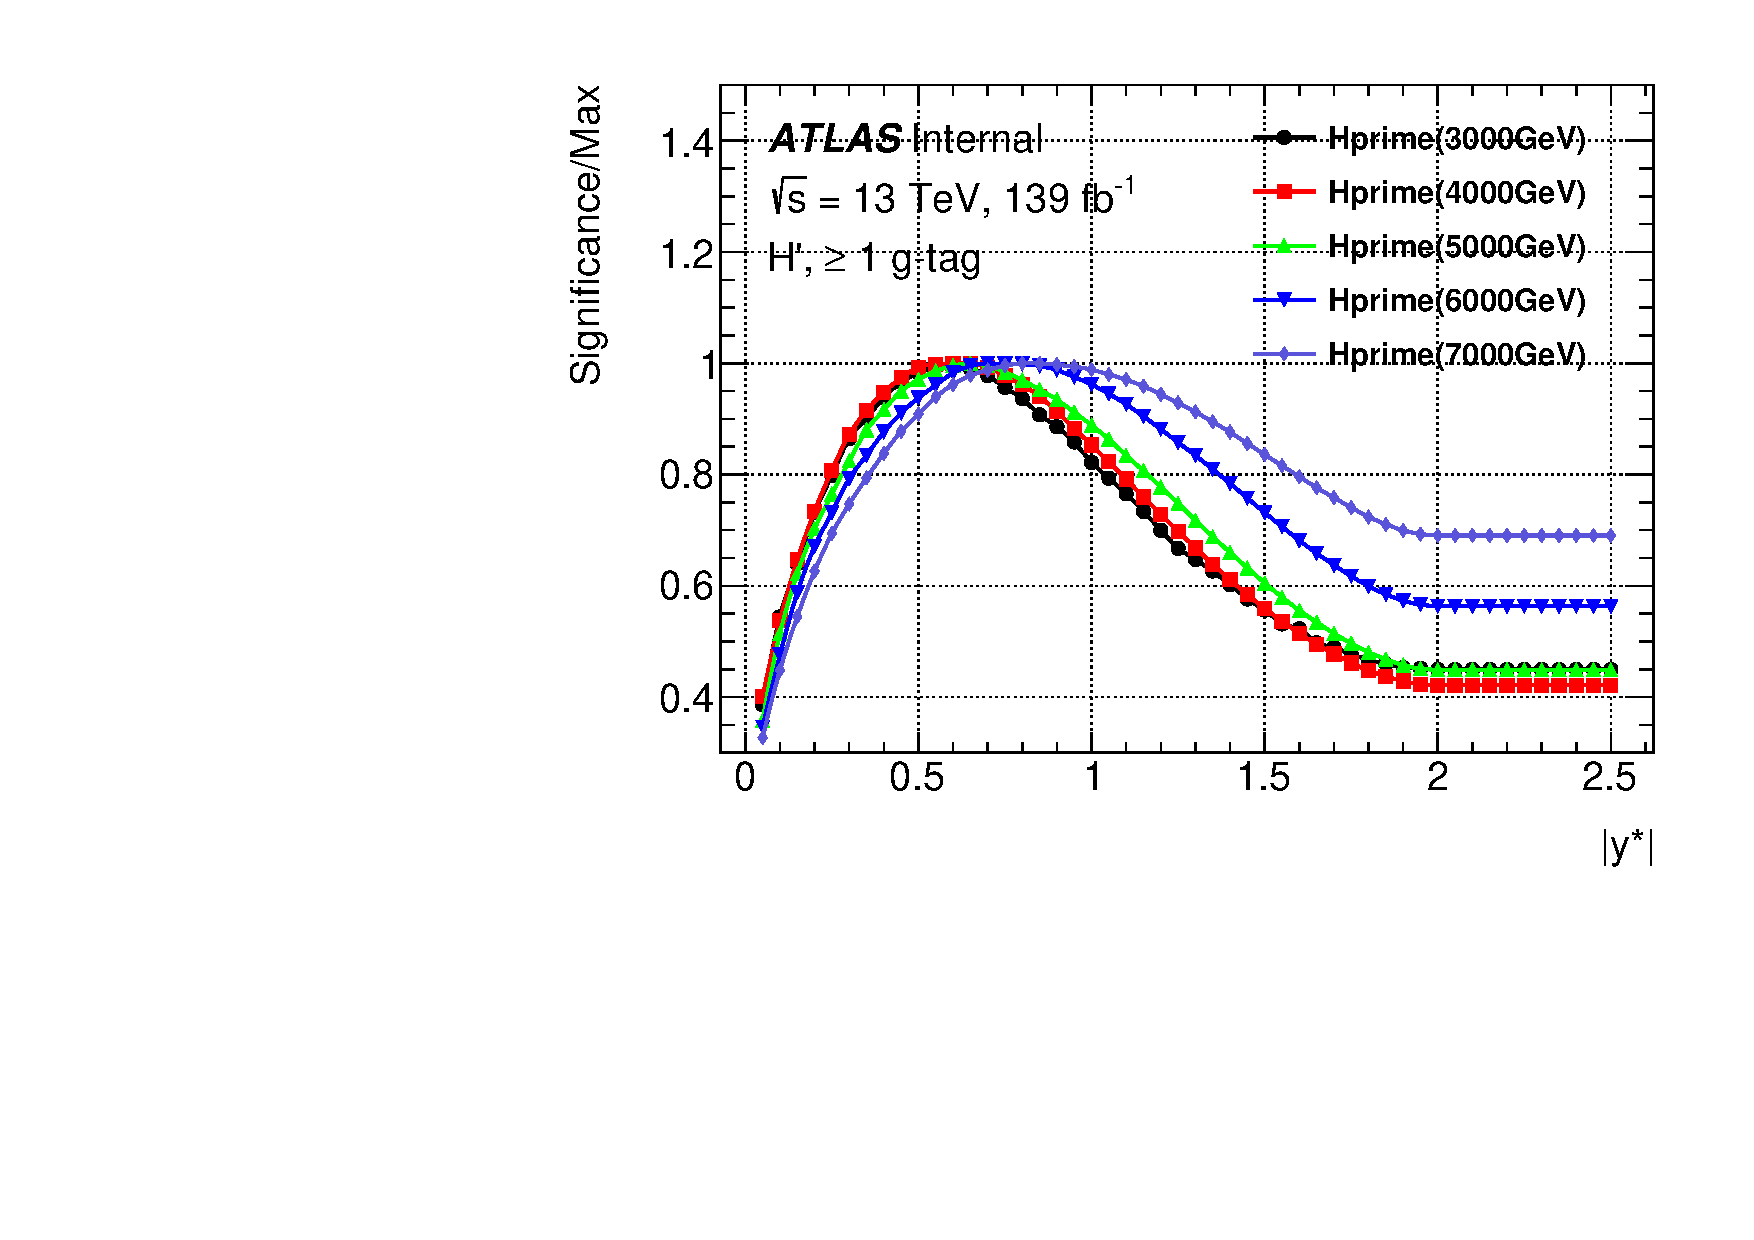
\includegraphics[width=0.48\columnwidth]{figures/yStarOptimization/Significance_Hprime_gj.pdf}}
        \subfigure[2 g-tag]{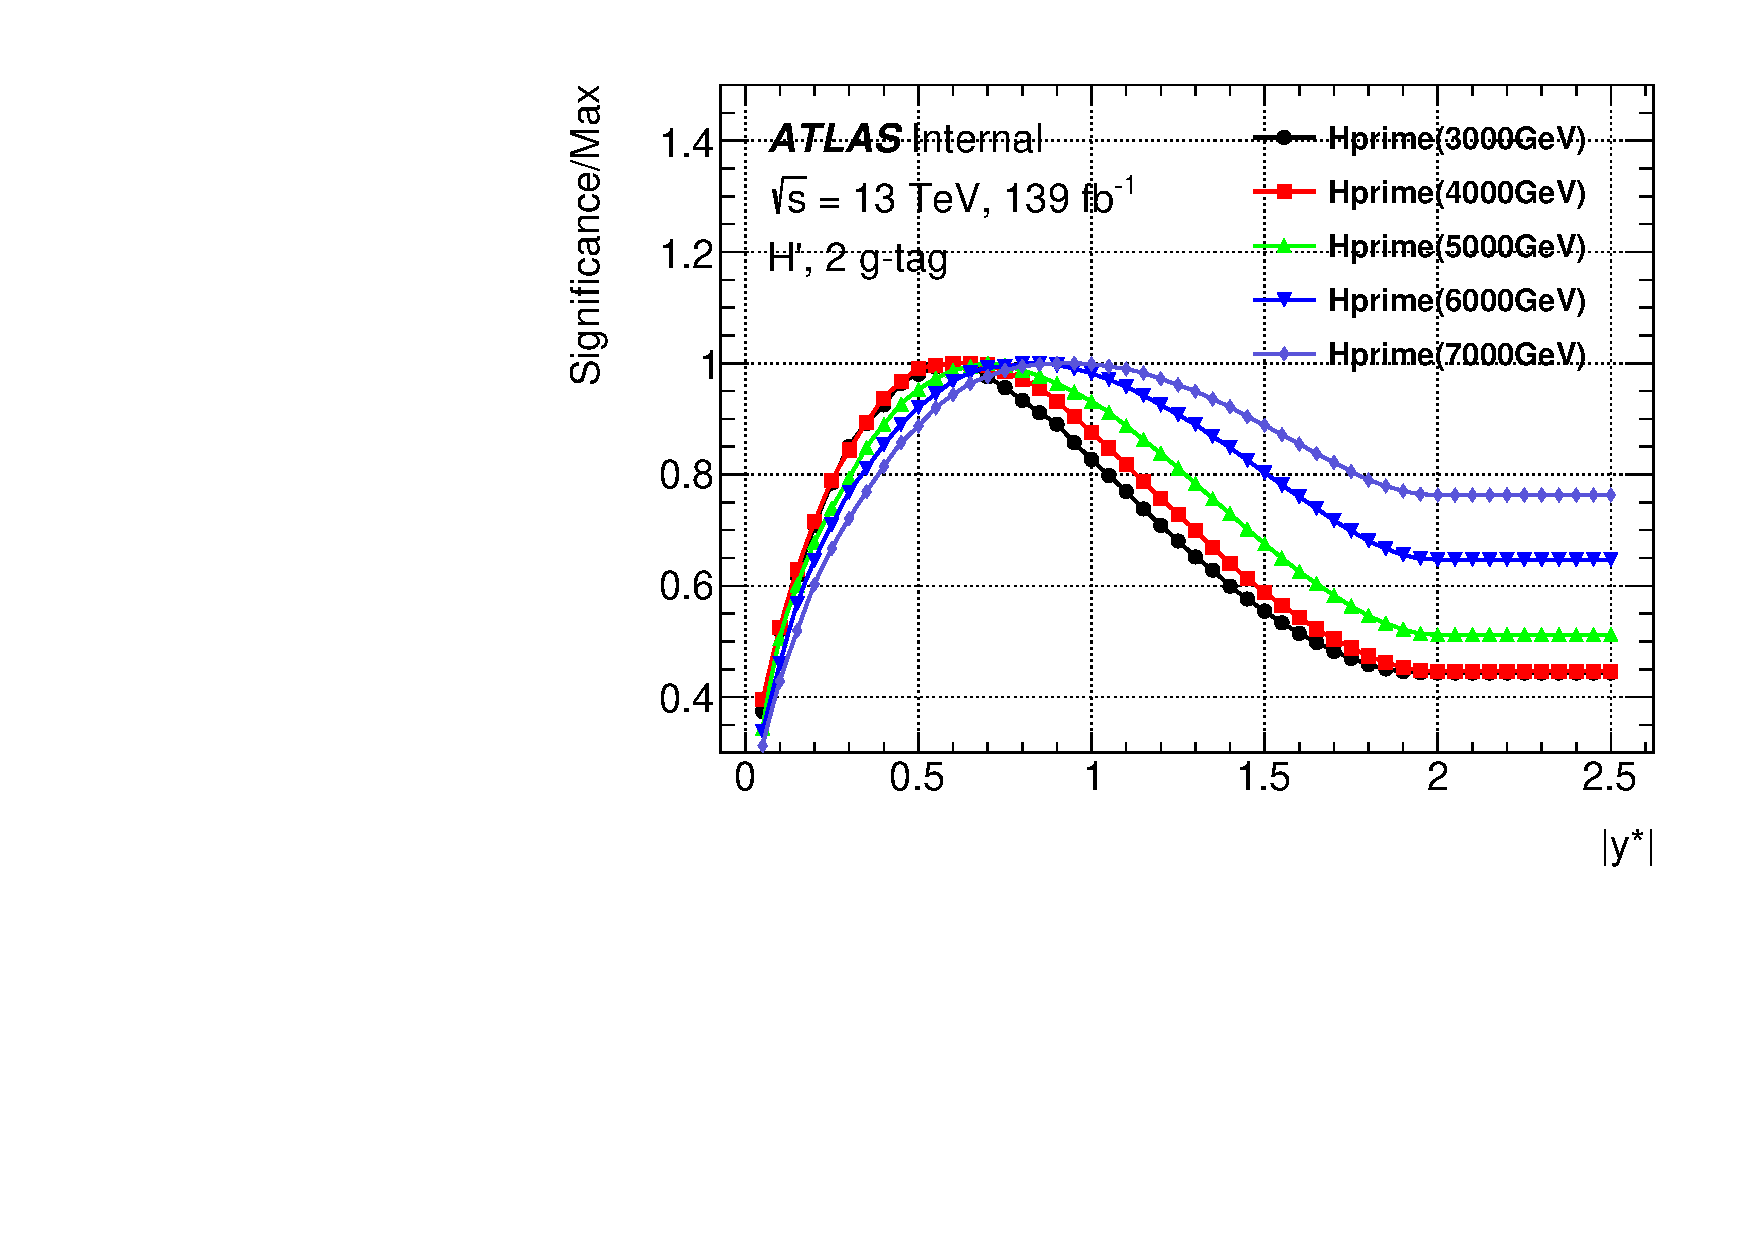
\includegraphics[width=0.48\columnwidth]{figures/yStarOptimization/Significance_Hprime_gg.pdf}}
        \caption{$H'$ significance as a function y* cut in the case of (a) $\geq$1 g-tag, (b) 2 g-tag.}
        \label{fig: hprime significance as a function of y* cut}
\end{figure}


\begin{figure}[htbp]
        \centering
        \subfigure[$\geq$1 g-tag]{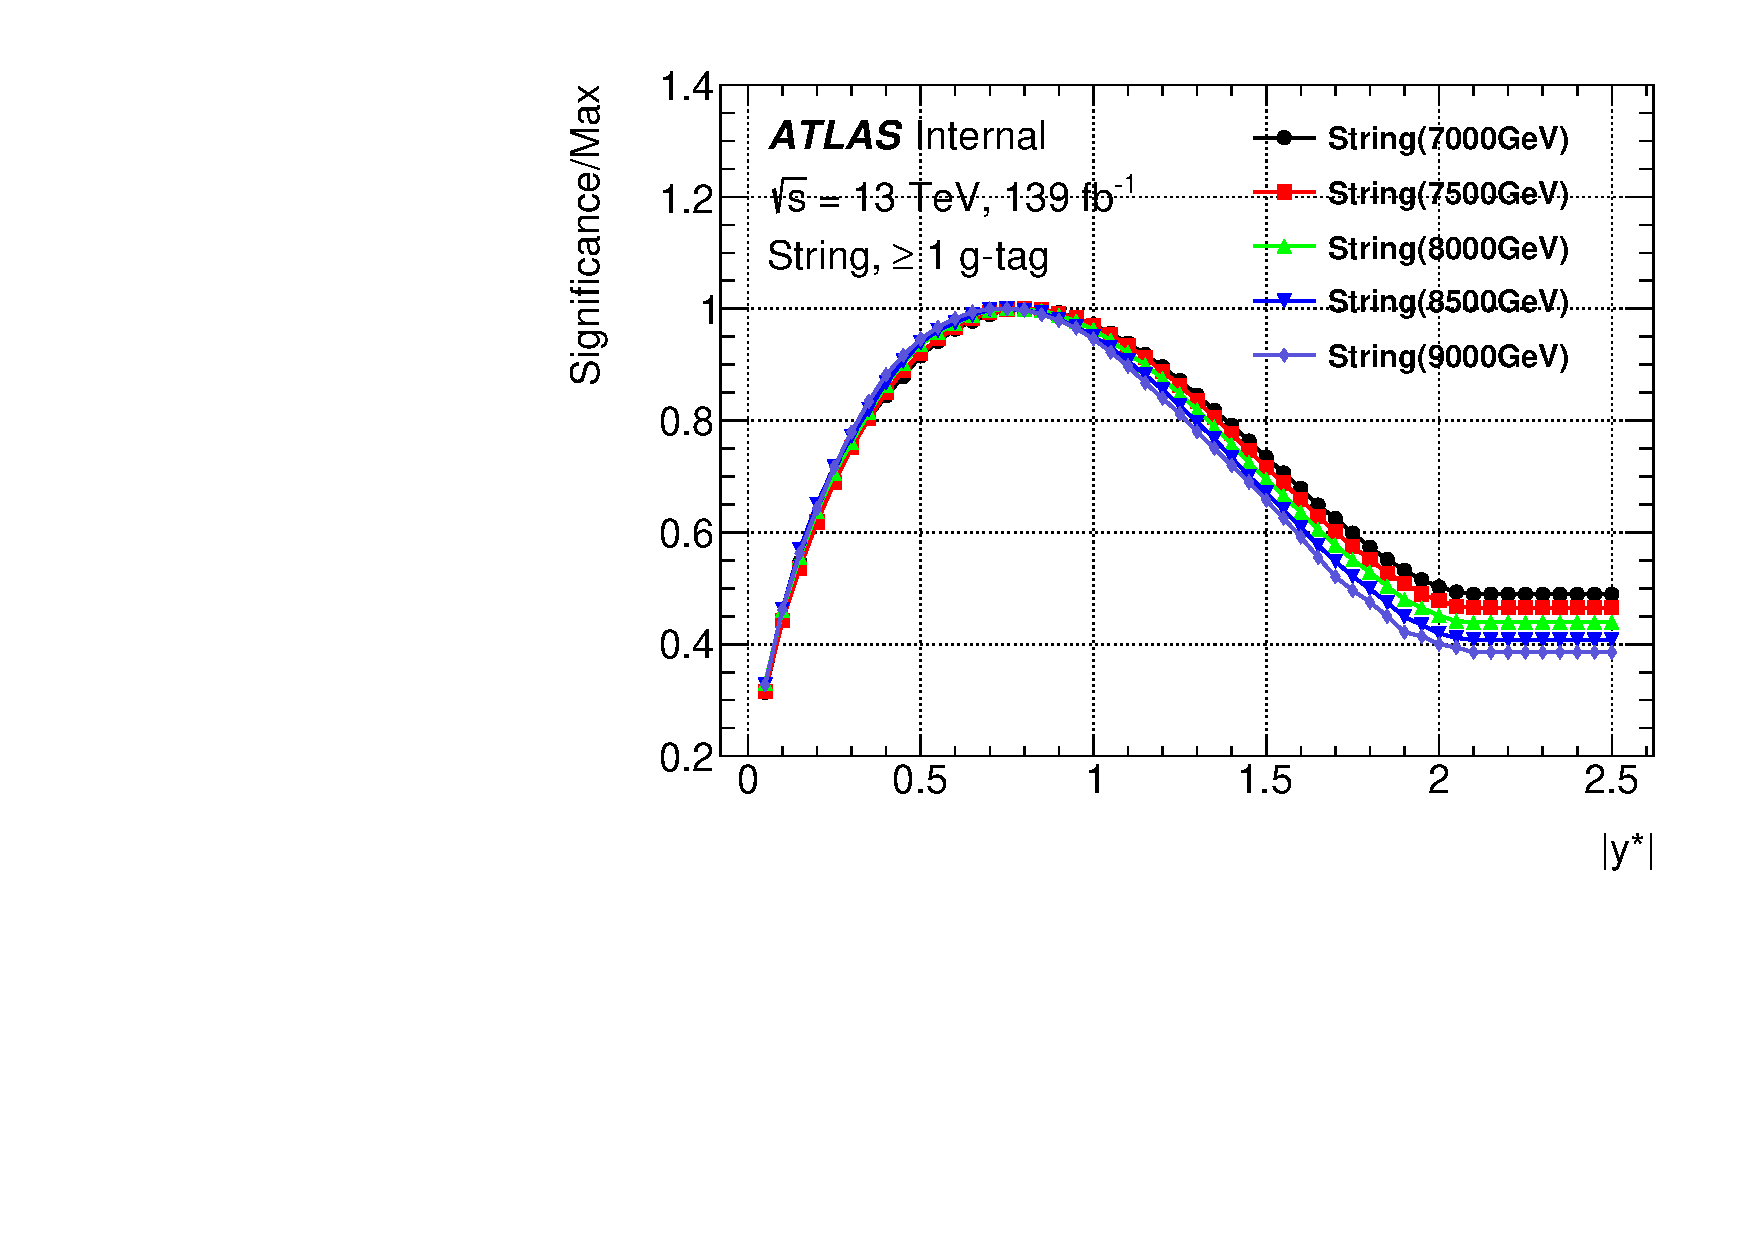
\includegraphics[width=0.48\columnwidth]{figures/yStarOptimization/Significance_String_gj.pdf}}
        \subfigure[2 g-tag]{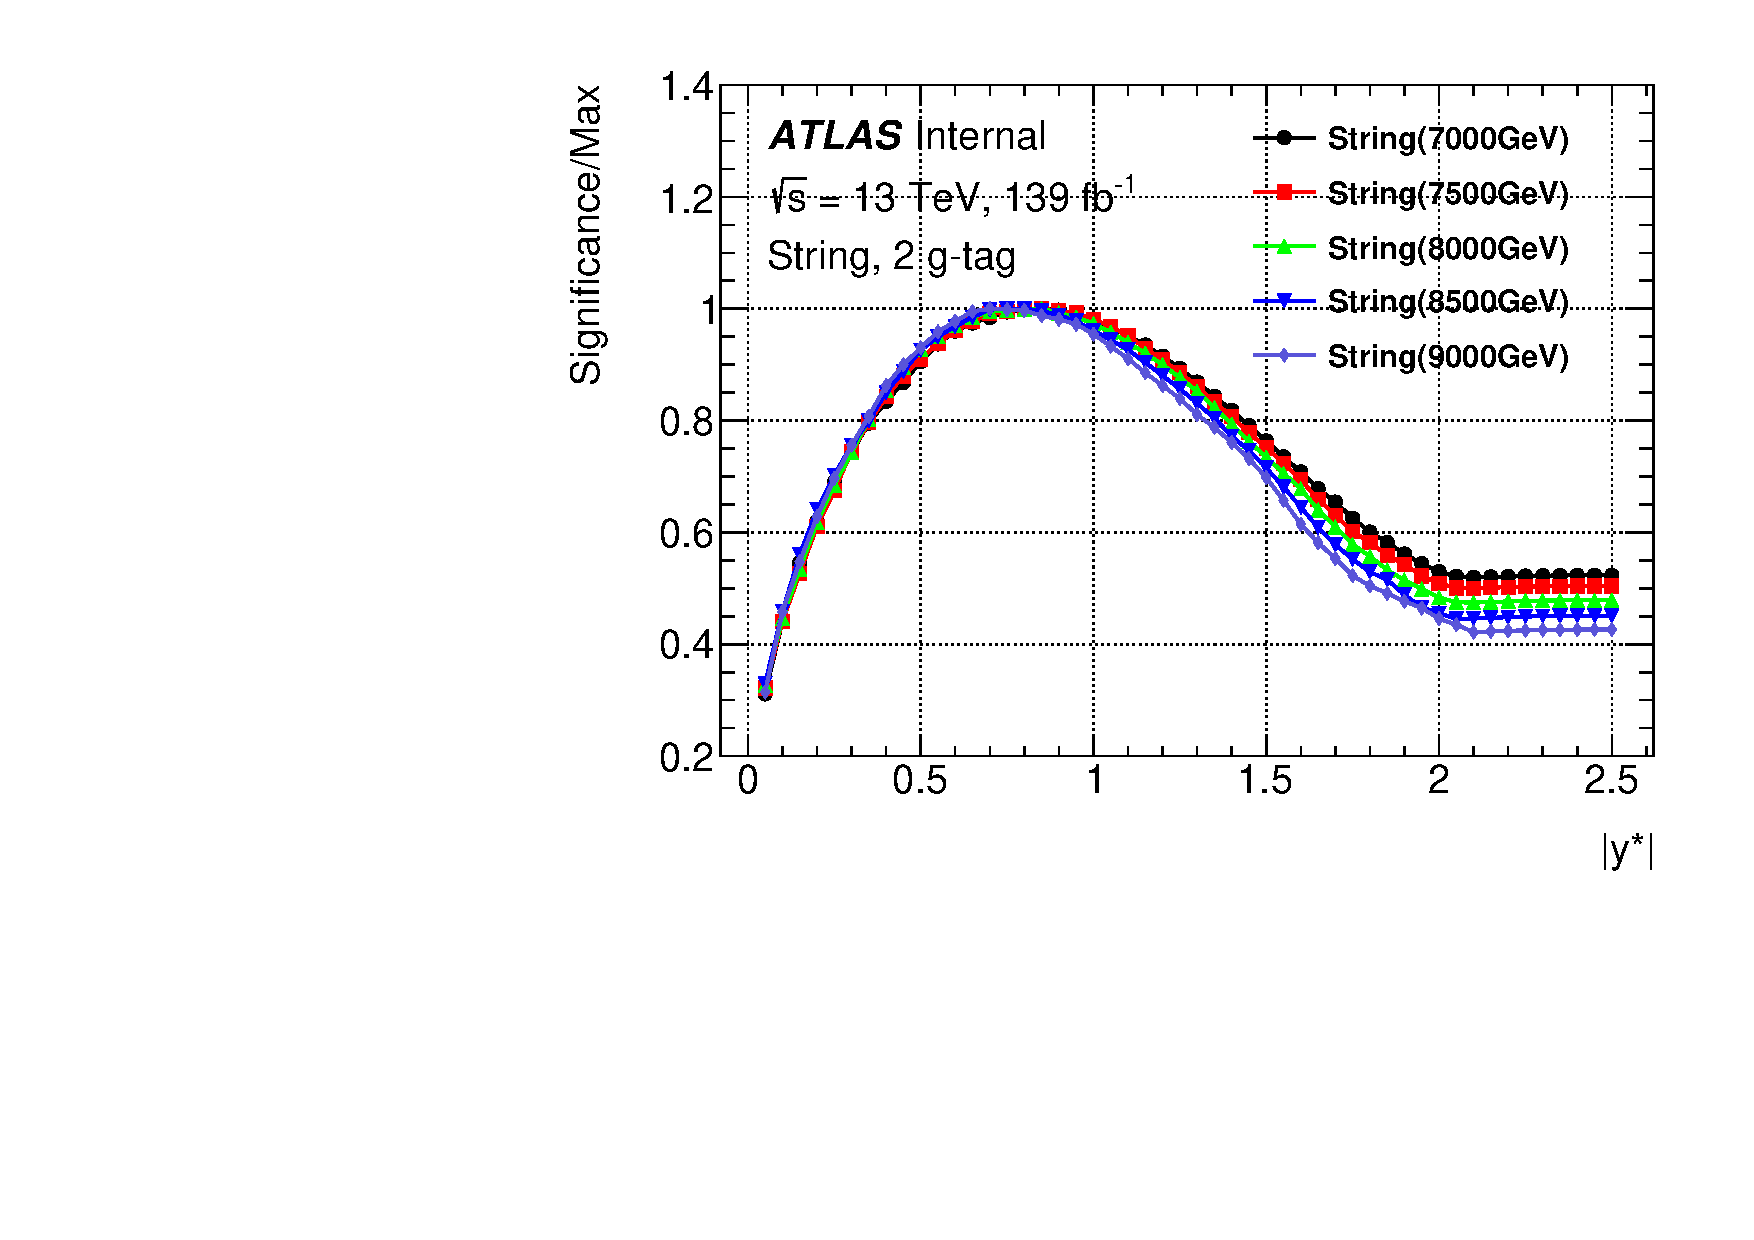
\includegraphics[width=0.48\columnwidth]{figures/yStarOptimization/Significance_String_gg.pdf}}
        \caption{$String$ significance as a function y* cut in the case of (a) $\geq$1 g-tag, (b) 2 g-tag.}
        \label{fig: string significance as a function of y* cut}
\end{figure}


\subsection{dijet mass turn-on}
\label{section: dijet mass turn-on}

The lowest single jet un-prescaled trigger in 2015 was HLT\_j360, in 2016 was HLT\_j380,
in 2017 and 2018 is HLT\_j420 which is avaliable in full Run 2 data.
The trigger selection will will bias the mass spectrum at low mass region, to avoid this bias, so an additional mass cut will be appied. 

To measure the $m_{jj}$ turn-on in data, an unbiased sample was obtained using the HLT\_j360 trigger, only data collected in 2015 corresponding to 3.2 $fb^{-1}$ is used in this measuerment.

Figure \ref{fig: mass turn-on yStar 0.6} shows the efficiencies as a function of $m_{jj}$ for $|y^{*}|<0.6$ in two g-tag regions, applying directly either triggers, respectively. The $m_{jj}$ value of the plateau ($\geq$99.5\%) is 1100 GeV. Figure \ref{fig: mass turn-on yStar 0.8} shows the efficiencies as a function of $m_{jj}$ for $|y^{*}|<0.8$ in two g-tag regions, the plateau value is 1200 GeV.

\begin{figure}[htbp]
        \centering
        \subfigure[$\geq$1 g-tag]{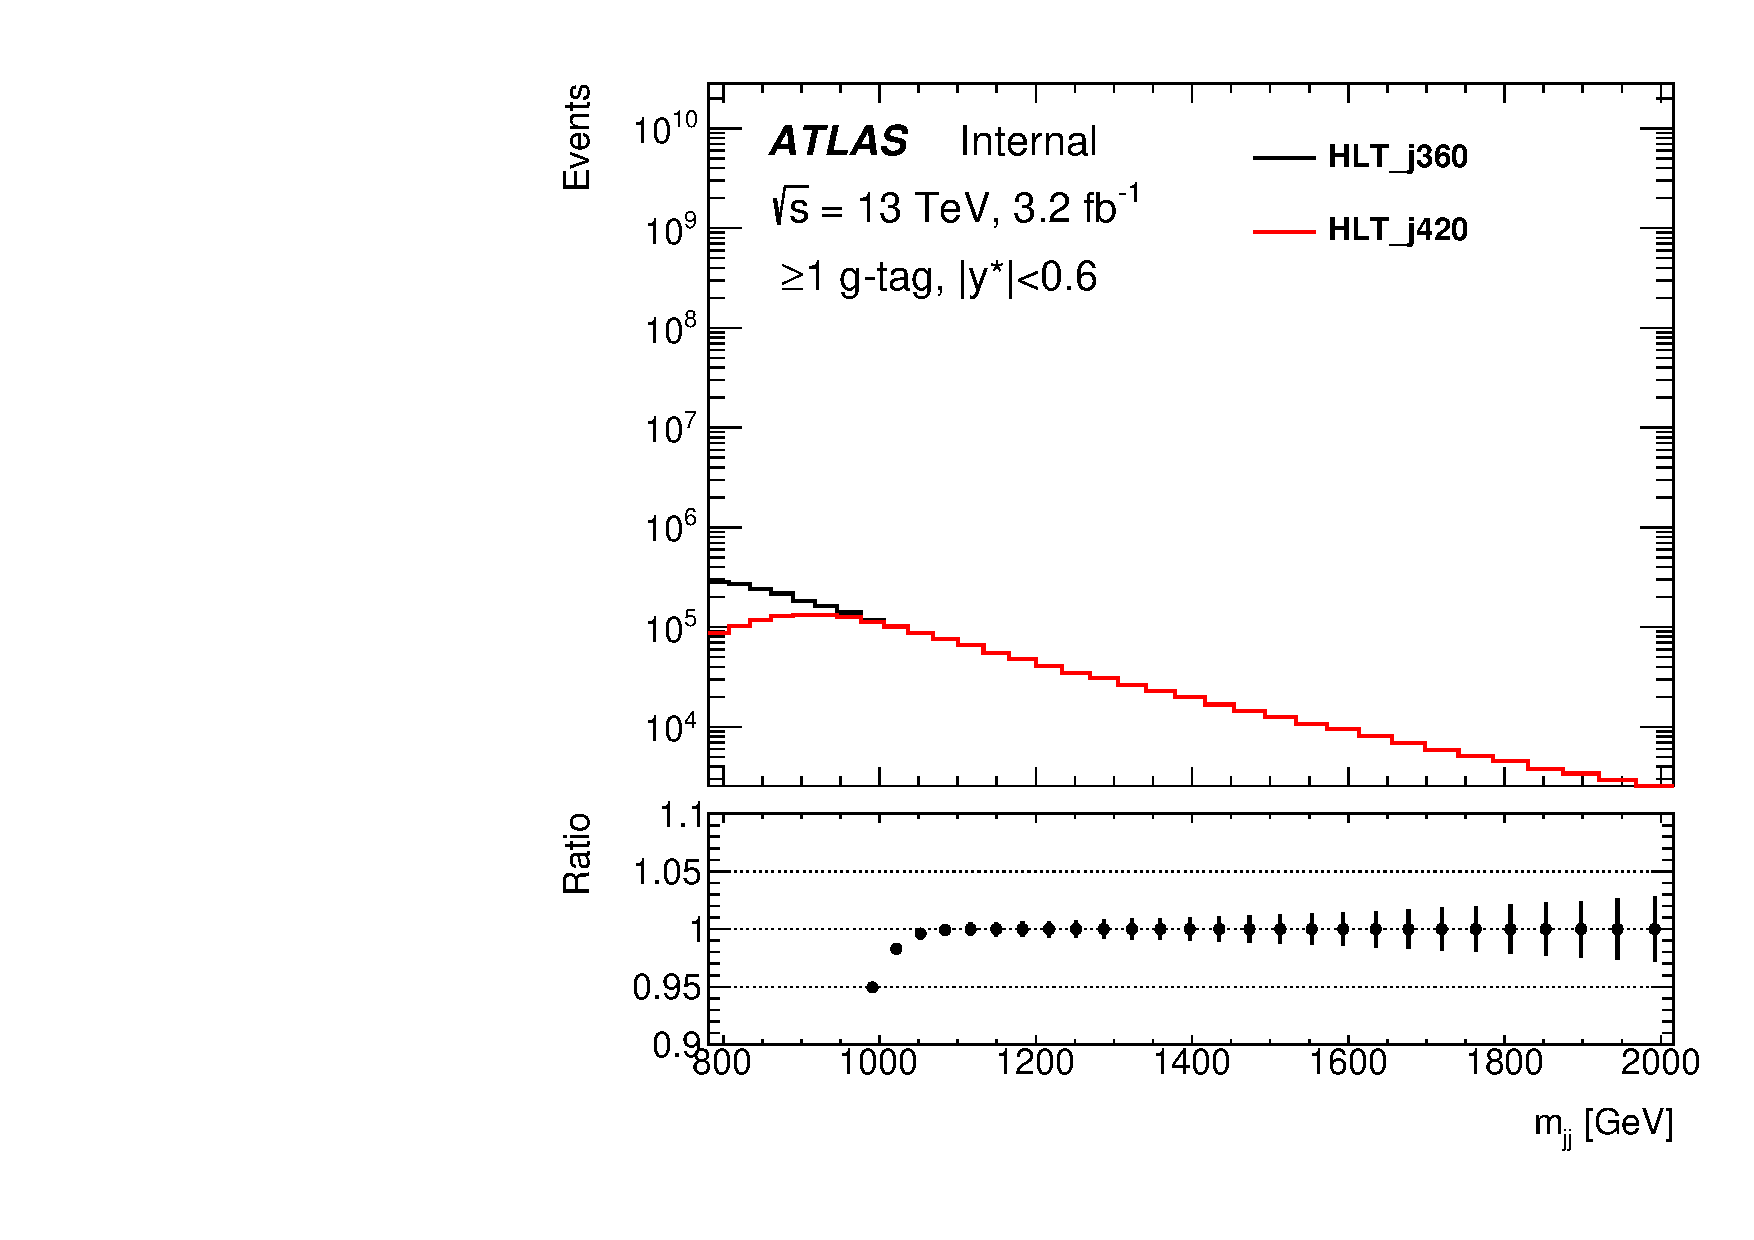
\includegraphics[width=0.48\columnwidth]{figures/massturnon/h_mass_gj_yStar0p6_ratio.pdf}}
        \subfigure[2 g-tag]{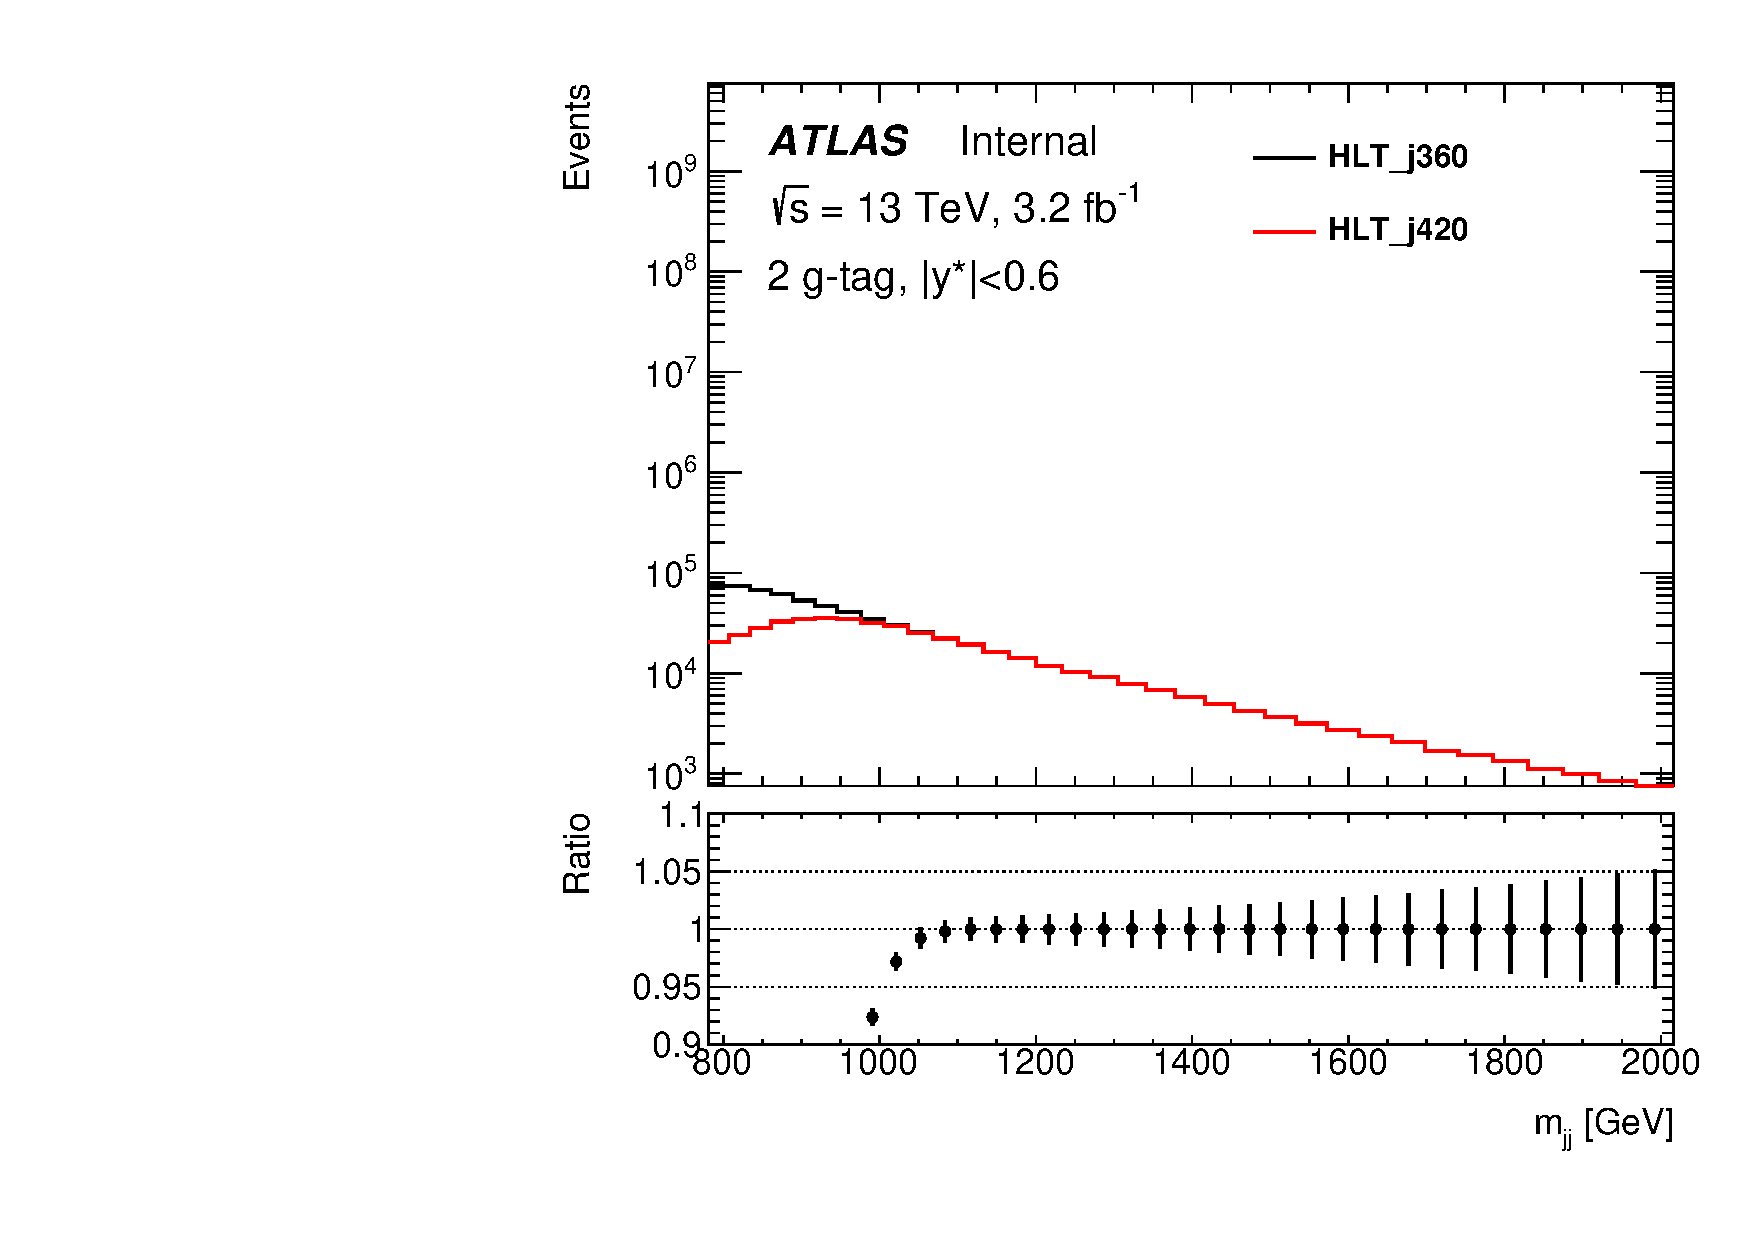
\includegraphics[width=0.48\columnwidth]{figures/massturnon/h_mass_gg_yStar0p6_ratio.pdf}}
        \caption{Efficiencies as a function of $m_{jj}$ for $y^{*}|<0.6$ using HLT\_j420 in the case of (a) $\geq$1 g-tag, (b) 2 g-tag.}
        \label{fig: mass turn-on yStar 0.6}
\end{figure}

\begin{figure}[htbp]
        \centering
        \subfigure[$\geq$1 g-tag]{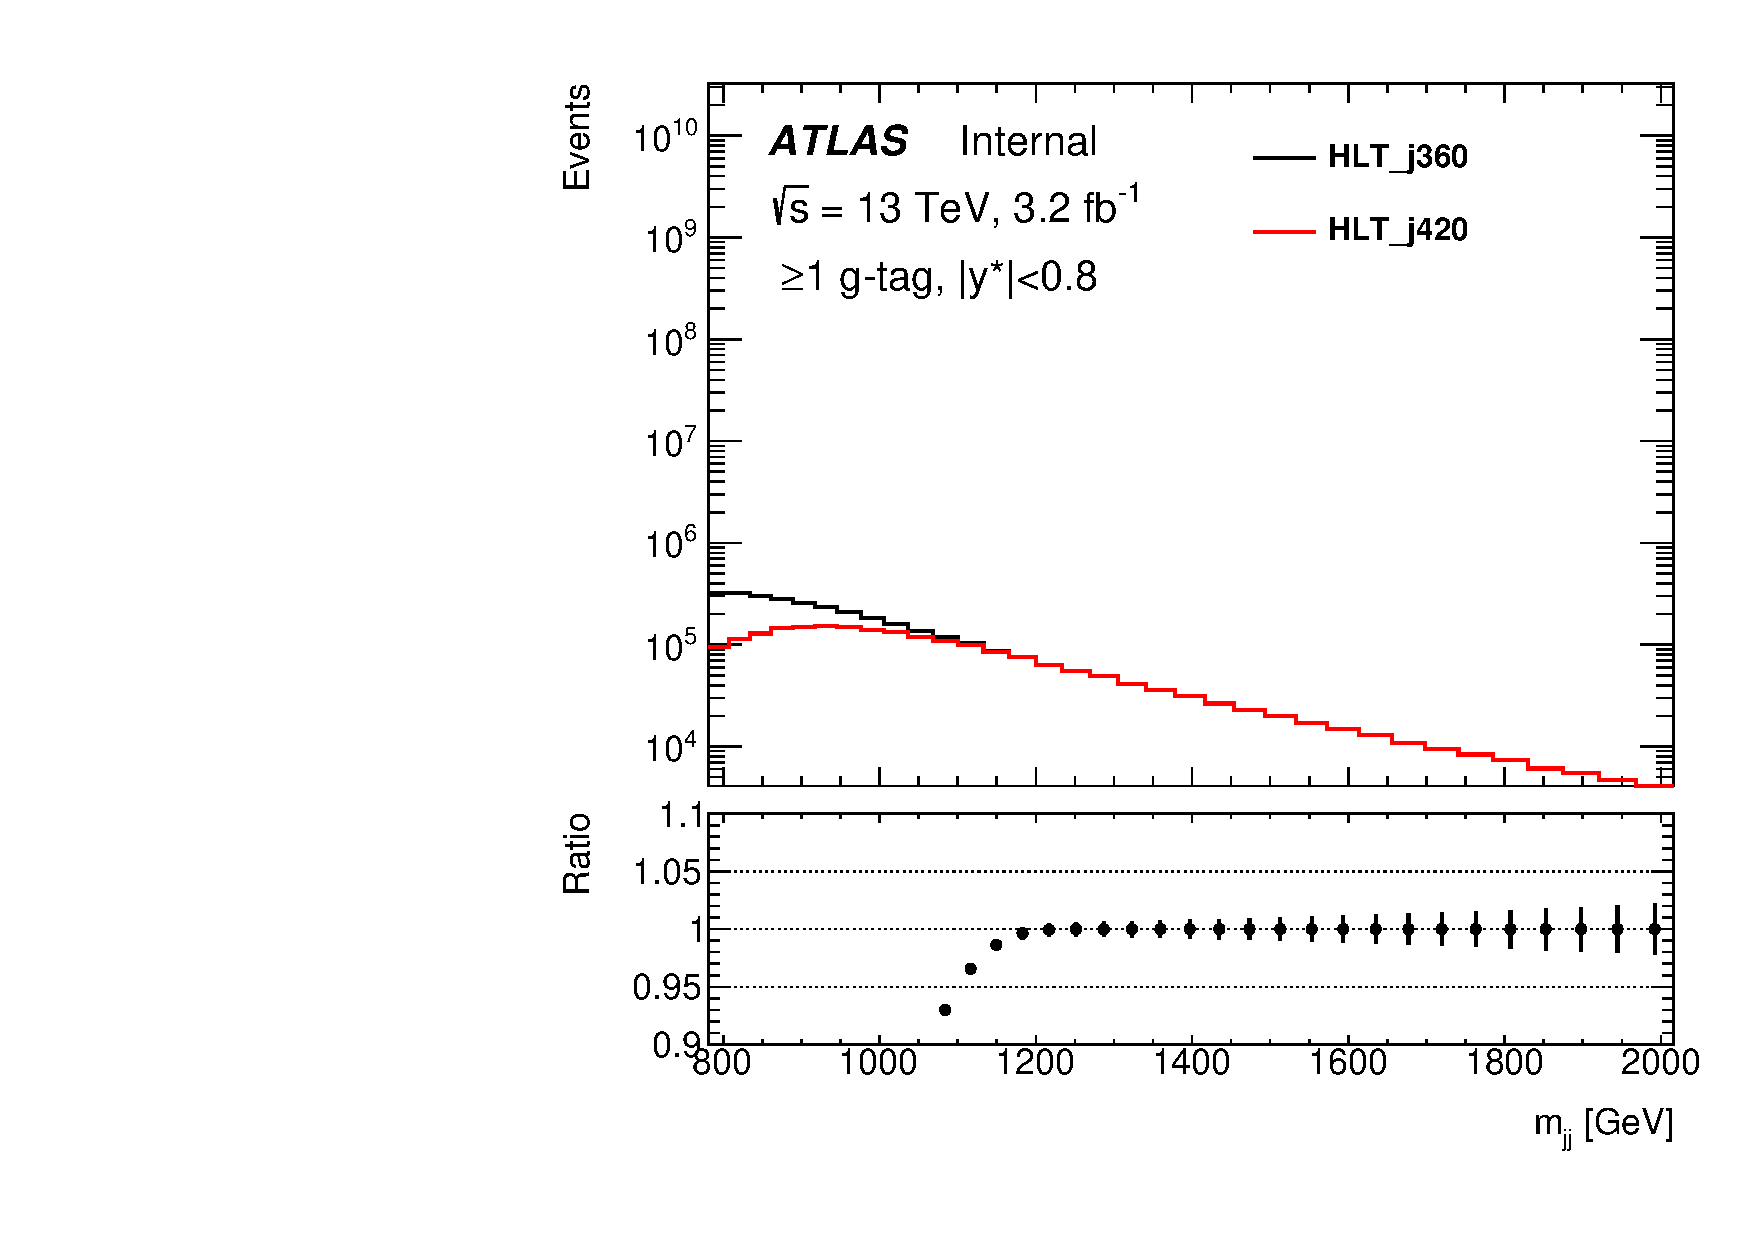
\includegraphics[width=0.48\columnwidth]{figures/massturnon/h_mass_gj_yStar0p8_ratio.pdf}}
        \subfigure[2 g-tag]{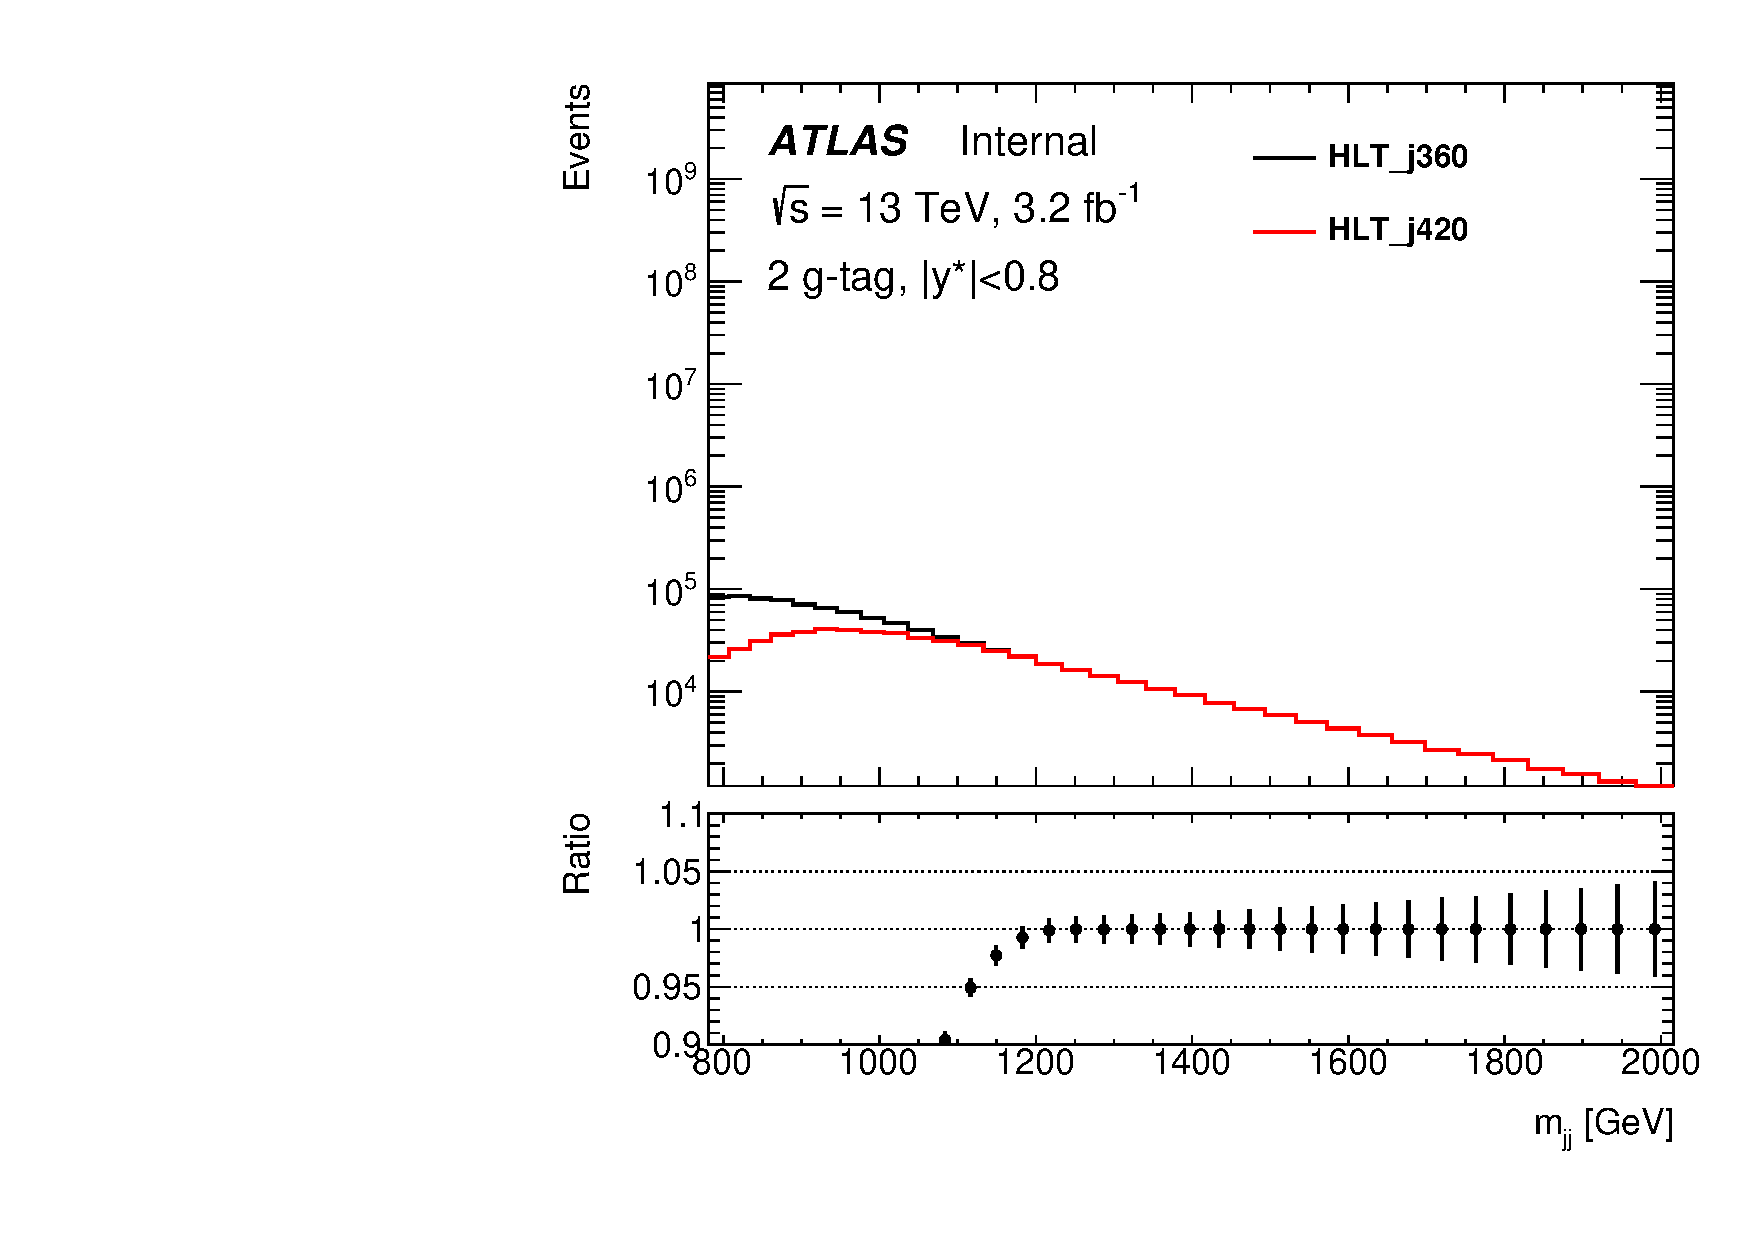
\includegraphics[width=0.48\columnwidth]{figures/massturnon/h_mass_gg_yStar0p8_ratio.pdf}}
        \caption{Efficiencies as a function of $m_{jj}$ for $y^{*}|<0.8$ using HLT\_j420 in the case of (a) $\geq$1 g-tag, (b) 2 g-tag.}
        \label{fig: mass turn-on yStar 0.8}
\end{figure}


\subsection{Baseline selection}
\label{sec:base_selection}
The baseline event selection is applied for all signal regions and
the cuts applied are:
\begin{itemize}
\item Good Run List (GRL): Requirement that all relevant detectors were in a good state ready for physics. The GRLs used for this analysis are:
	\begin{itemize}
		%\item 2015(3.2\,\ifb): data15\_13TeV.periodAllYear\_DetStatus-v89-pro21-02\_Unknown\_PHYS\_ \newline StandardGRL\_All\_Good\,\_25ns.xml
		%\item 2016(32.97\,\ifb): data16\_13TeV.periodAllYear\_DetStatus-v89-pro21-01\_DQDefects-00-02-04\_ \newline PHYS\_StandardGRL\_All\_Good\_25ns.xml
		%\item 2017(44.31\,\ifb): data17\_13TeV.periodAllYear\_DetStatus-v99-pro22-01\_Unknown\_ \newline PHYS\_StandardGRL\_All\_Good\_25ns\_Triggerno17e33prim.xml
		%\item 2018(59.94\,\ifb): data18\_13TeV.periodAllYear\_DetStatus-v102-pro22-04\_Unknown\_PHYS\_ \newline StandardGRL\_All\_Good\_25ns\_Triggerno17e33prim.xml
                \item 2015(3.2 ~\ifb): data15\_13TeV.periodAllYear\_DetStatus-v89-pro21-02\_Unknown\_PHYS\\\_StandardGRL\_All\_Good\_25ns.xml
        	\item 2016(33 ~\ifb): data16\_13TeV.periodAllYear\_DetStatus-v89-pro21-01\_DQDefects-00-02-04\_PHYS\\\_StandardGRL\_All\_Good\_25ns.xml
        	\item 2017(44.2 ~\ifb): data17\_13TeV.periodAllYear\_DetStatus-v99-pro22-01\_Unknown\_PHYS\\\_StandardGRL\_All\_Good\_25ns\_JetHLT\_Normal2017.xml
        	\item 2018(58.5 ~\ifb): data18\_13TeV.periodAllYear\_DetStatus-v102-pro22-04\_Unknown\_PHYS\\\_StandardGRL\_All\_Good\_25ns\_Triggerno17e33prim.xml
	\end{itemize}
\item LAr: Liquid Argon Calorimeter error rejected ( errorState(xAOD::EventInfo::LAr) )
\item Tile: Tile Calorimeter error rejected ( errorState(xAOD::EventInfo::Tile) )
\item SCT: SCT single event upsets rejected ( errorState(xAOD::EventInfo::SCT) )
\item Core: Incomplete event build rejected ( isEventFlagBitSet(xAOD::EventInfo::Core, 18) )
\item All jets with $\pt\ge 150~\GeV$ pass LooseBad cleaning cuts
\item Primary Vertex: the highest $\sum\pt^{2}(trk)$ (xAOD::VxType::VertexType::PriVtx) vertex has at least two tracks associated with it
\item Trigger: Passes the lowest unprescaled single-jet trigger, HLT\_j420
\item Jet preselecton: Leading jet $\pt\ge 380~\GeV$ and Jet multiplicity $\ge 2$
\end{itemize}

Additional kinematic selection criteria are used for the resonance to optimise the search potential and ensure good tracking efficiency. 

The following cuts are applied to the H$^\prime$ search.
\begin{itemize}
\item $|\Delta\phi| > 1.0$
\item $|\ystar| < 0.6$
\item $\mjj > 1100~\GeV$
\end{itemize}

The following cuts are applied to the string resonace search.
\begin{itemize}
\item $|\ystar| < 0.8$
\item $\mjj > 1717~\GeV$
\end{itemize}

The above cuts define the inclusive samples.
The following additonal cuts are for quark-gluon tagging.
\begin{itemize}
\item $|\eta| < 0.21$ (both jets)
\item $\ge 1$ gluon tagged (75\% working point)
\item 2 gluons tagged (75\% working point)
\end{itemize}

\noindent
where the 75\% gluon selecton criteria is $n{500} > -7.26742 + 4.16218\ln(\pt)$.

\subsection{Basic kinematic plots}
\label{sec:kinematic_distributions}

%In this section a selection of kinematic and monitoring plots produced with the resonant selection on the full dataset is shown 
%(Figures~\ref{fig:monitoring1}, %\ref{fig:monitoring2}, \ref{fig:monitoring3}, 
%\ref{fig:monitoring5}, \ref{fig:monitoring6}). These plots are relative to \integLumi of data collected in 2015 and 2016.
% GRL has been applied here.
%
%\begin{figure}[htb]
% \centering
% \subfigure[] {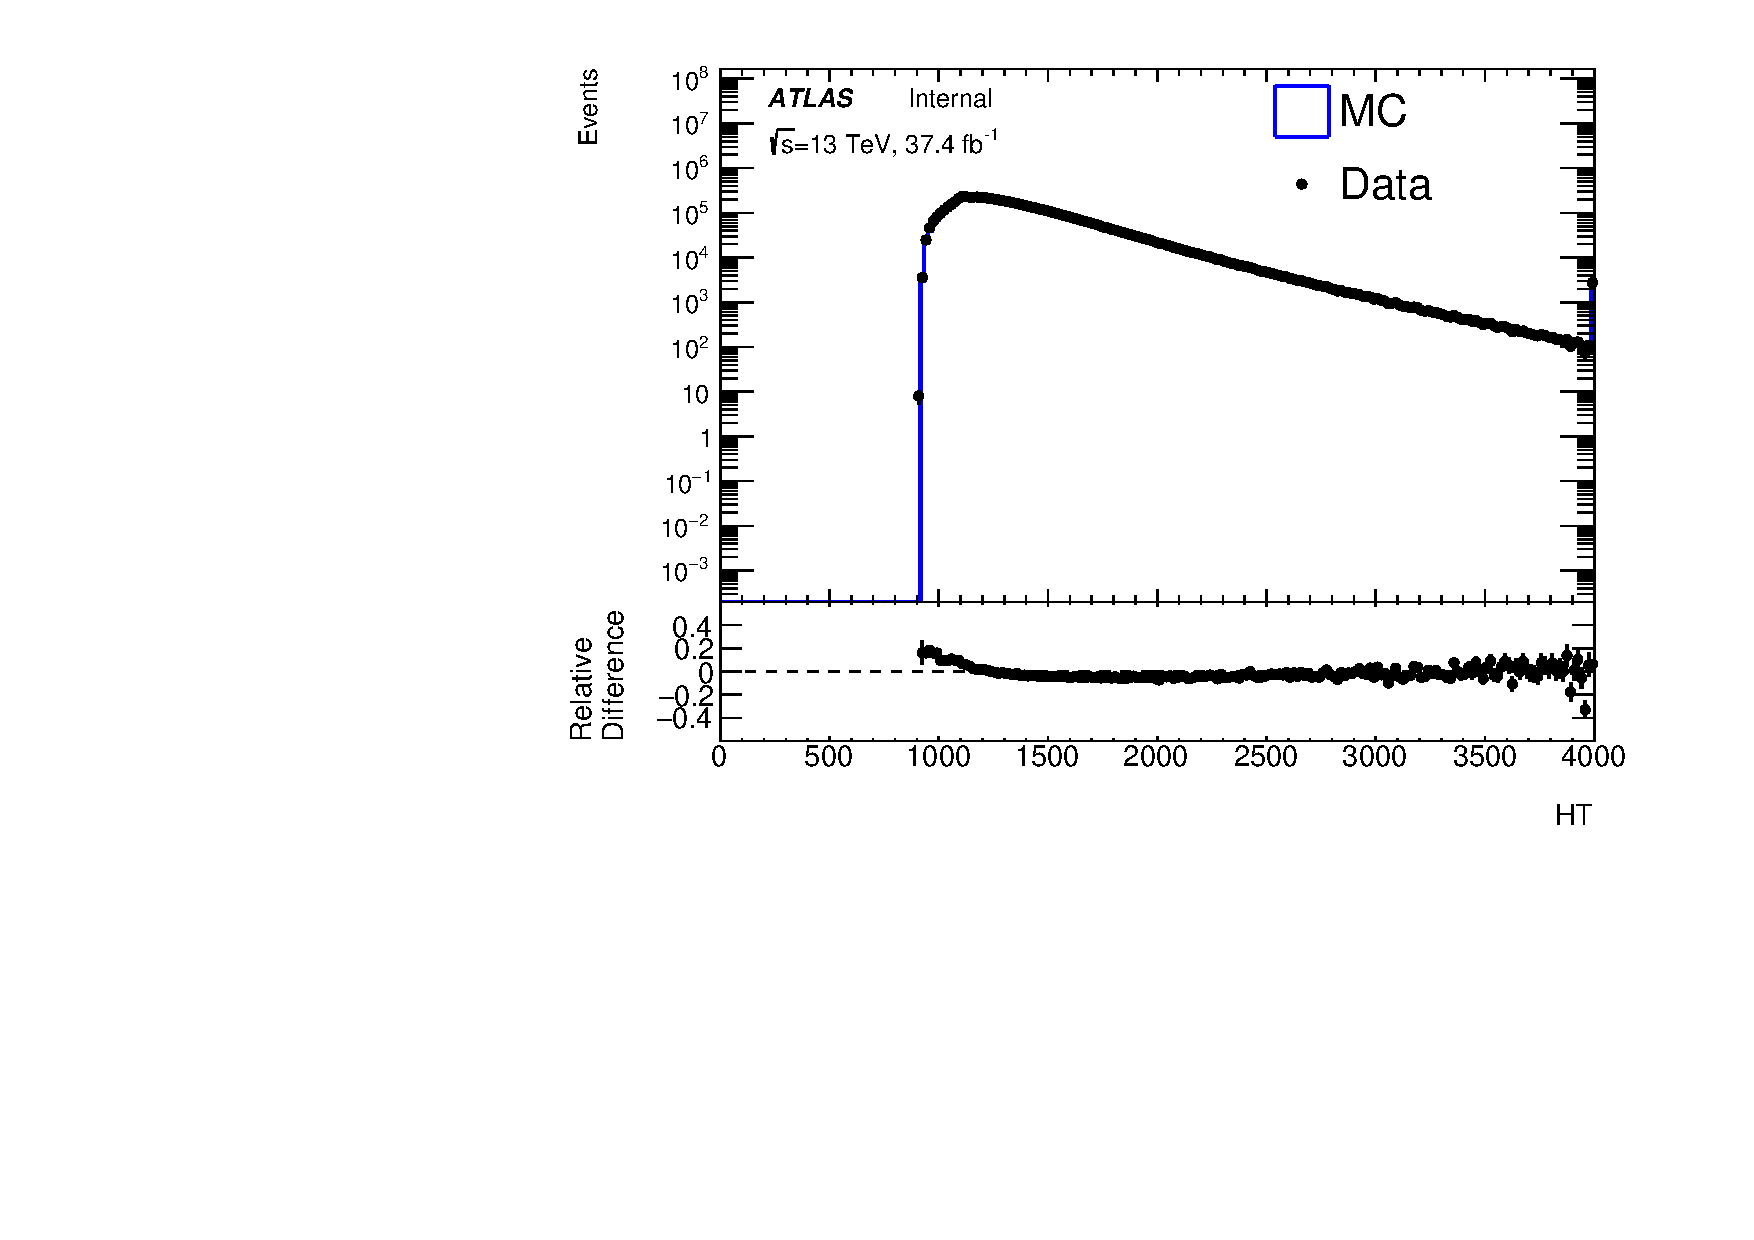
\includegraphics[width=0.45\textwidth]{figures/monitoring/resonant/Moriond_2017/newStudy_HT_logY.pdf}}
% \subfigure[] {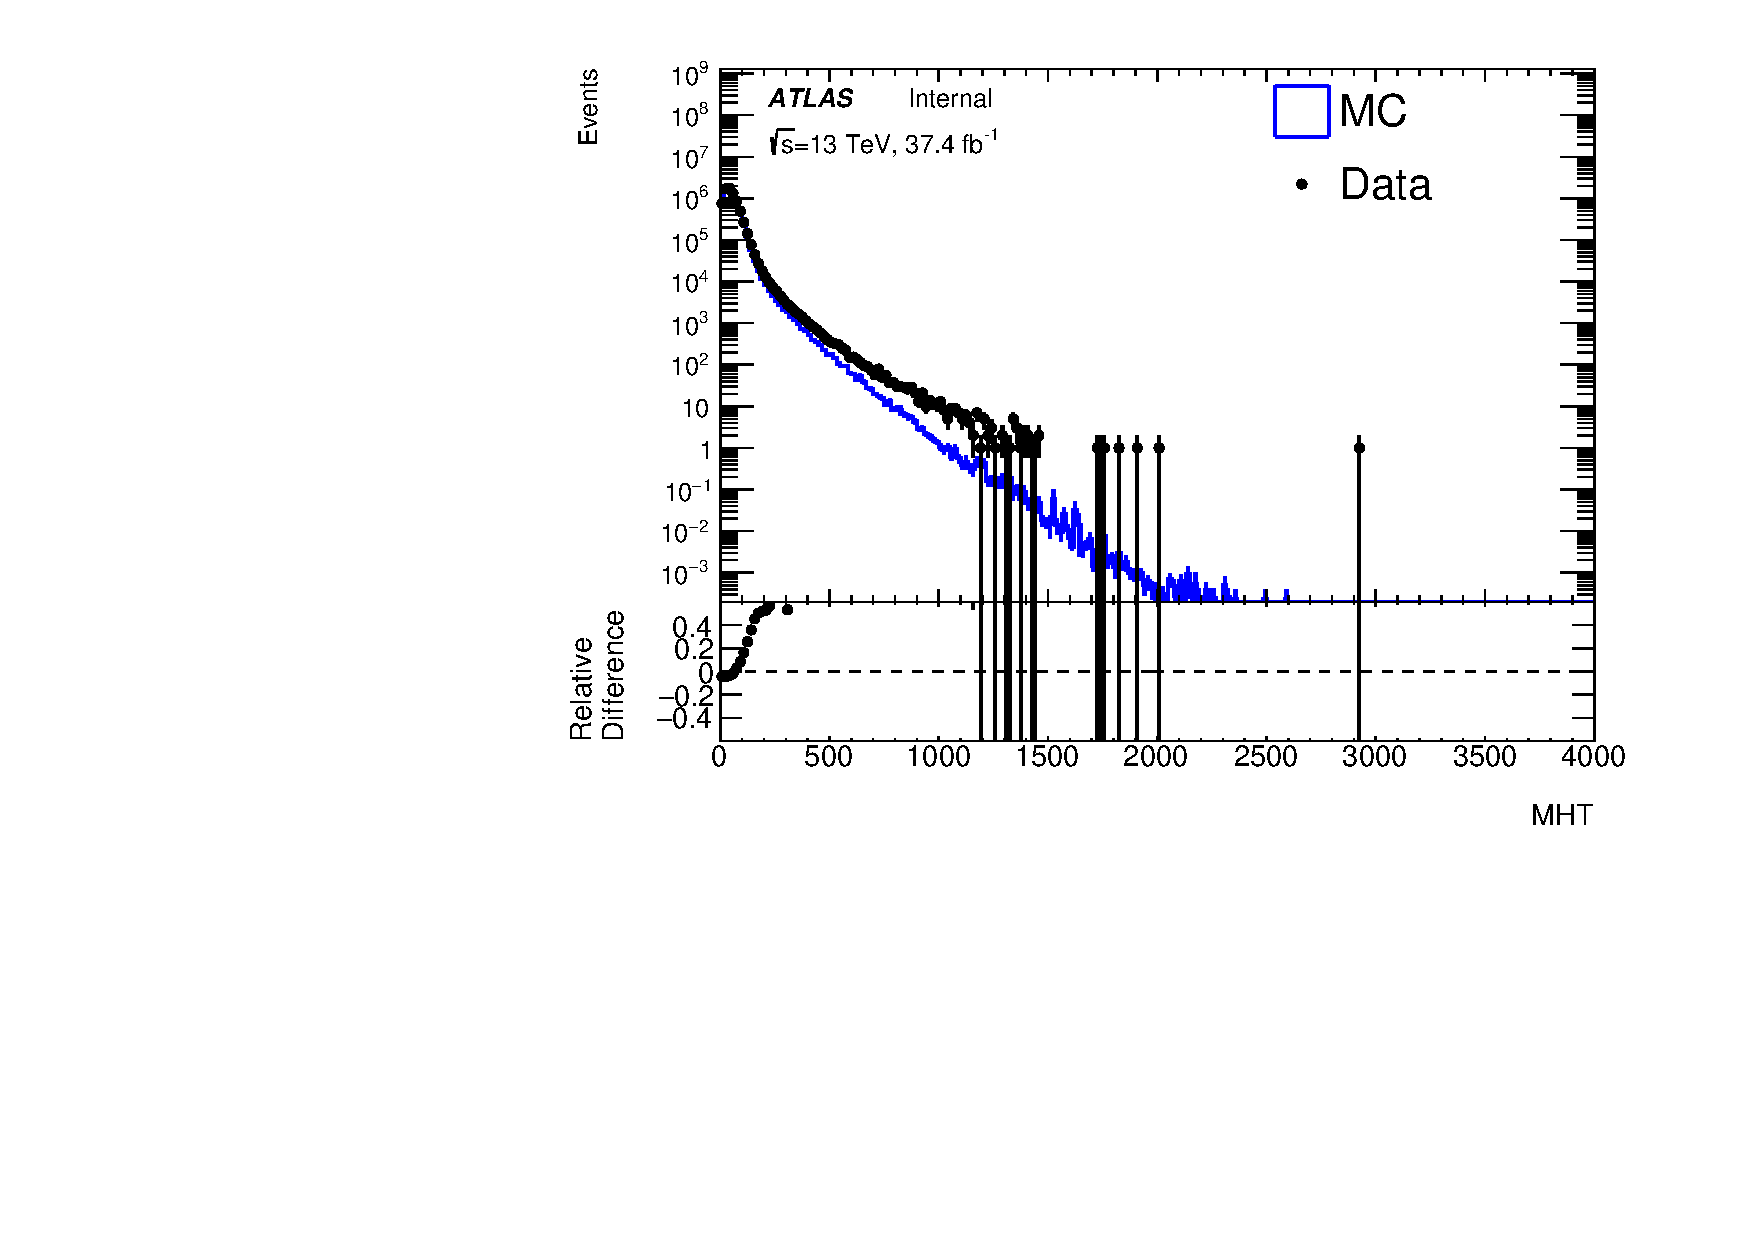
\includegraphics[width=0.45\textwidth]{figures/monitoring/resonant/Moriond_2017/newStudy_MHT_logY.pdf}}
% %
% \subfigure[] {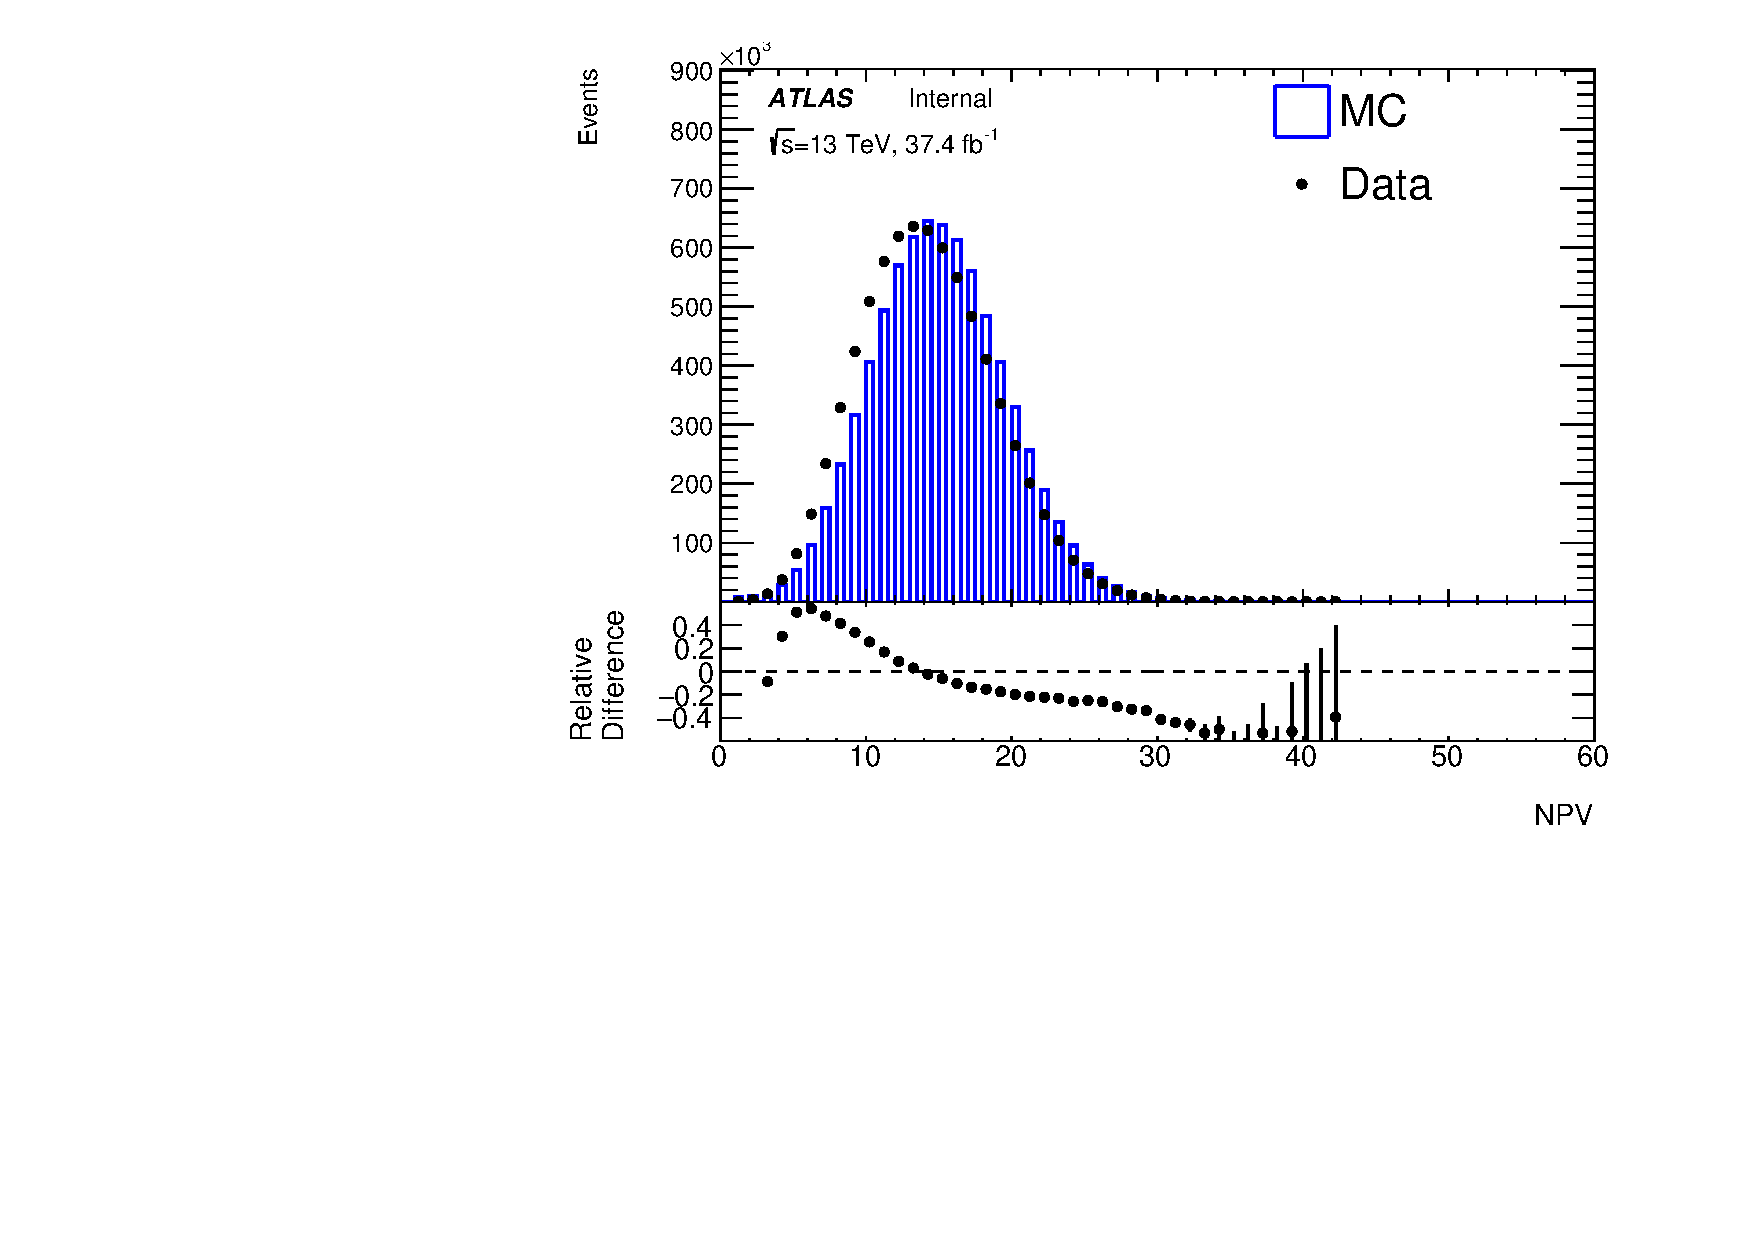
\includegraphics[width=0.45\textwidth]{figures/monitoring/resonant/Moriond_2017/newStudy_NPV.pdf}}
% \subfigure[] {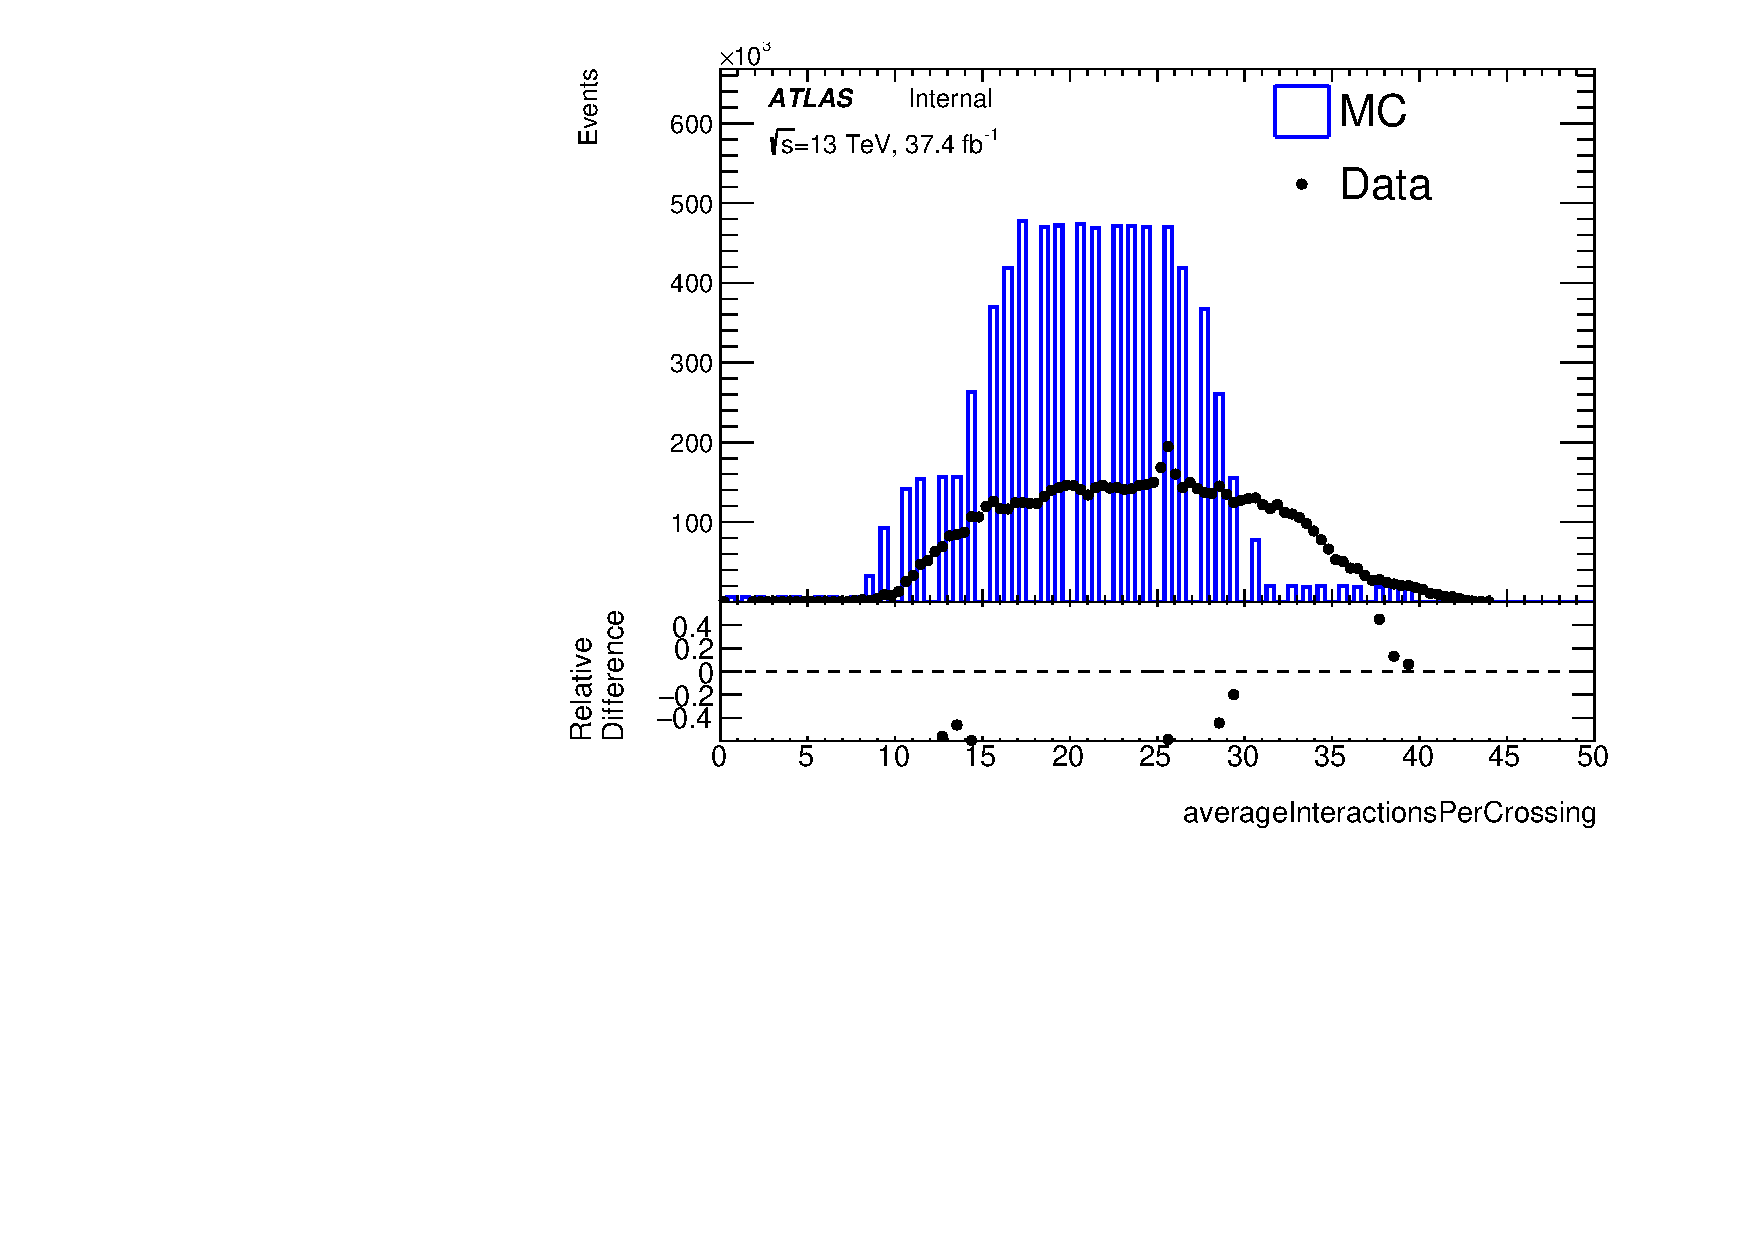
\includegraphics[width=0.45\textwidth]{figures/monitoring/resonant/Moriond_2017/newStudy_averageInteractionsPerCrossing.pdf}}
% \caption{Monitoring plots on %2016 data, 
% the resonant selection. (a) $H_T$, (b) $MH_T$ (missing transverse momentum calculated only from the jets in the event), (c) number of primary interaction vertices and (d) average interactions per bunch crossing.}
% \label{fig:monitoring1}
%\end{figure}
%
%
%\clearpage
%
%In this section a selection of kinematic and monitoring plots produced with the resonant selection on the complete resonance dataset is shown 
%(Figures~\ref{fig:JJmonitoring1},  
%\ref{fig:JJmonitoring5}, \ref{fig:JJmonitoring6}). These plots are relative to \integLumi of data collected in 2015 and 2016.
% GRL has been applied here.
%
%
%\begin{figure}[htb]
% \centering
% \subfigure[] {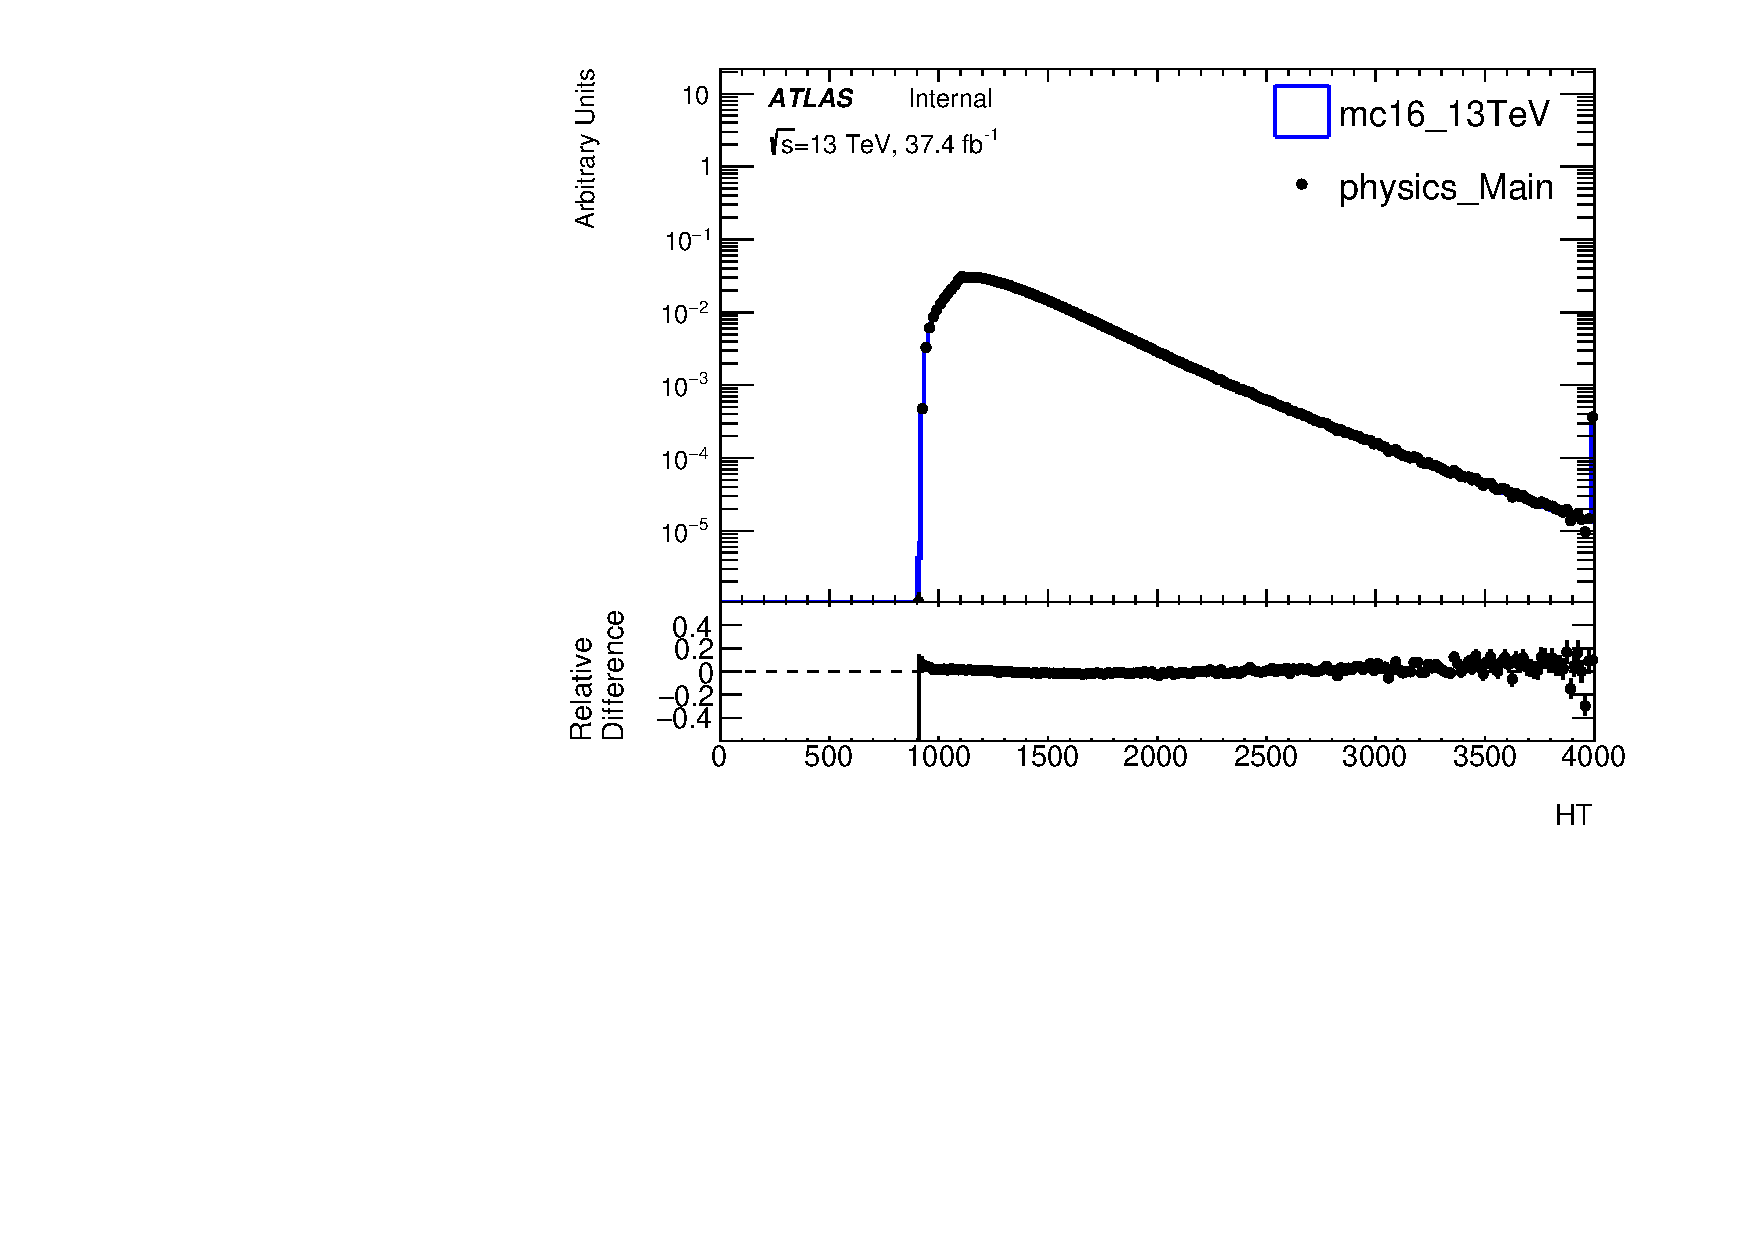
\includegraphics[width=0.45\textwidth]{figures/monitoring/resonant/2015-16/JJ/newStudy_HT_logY_JJv01.pdf}}
% \subfigure[] {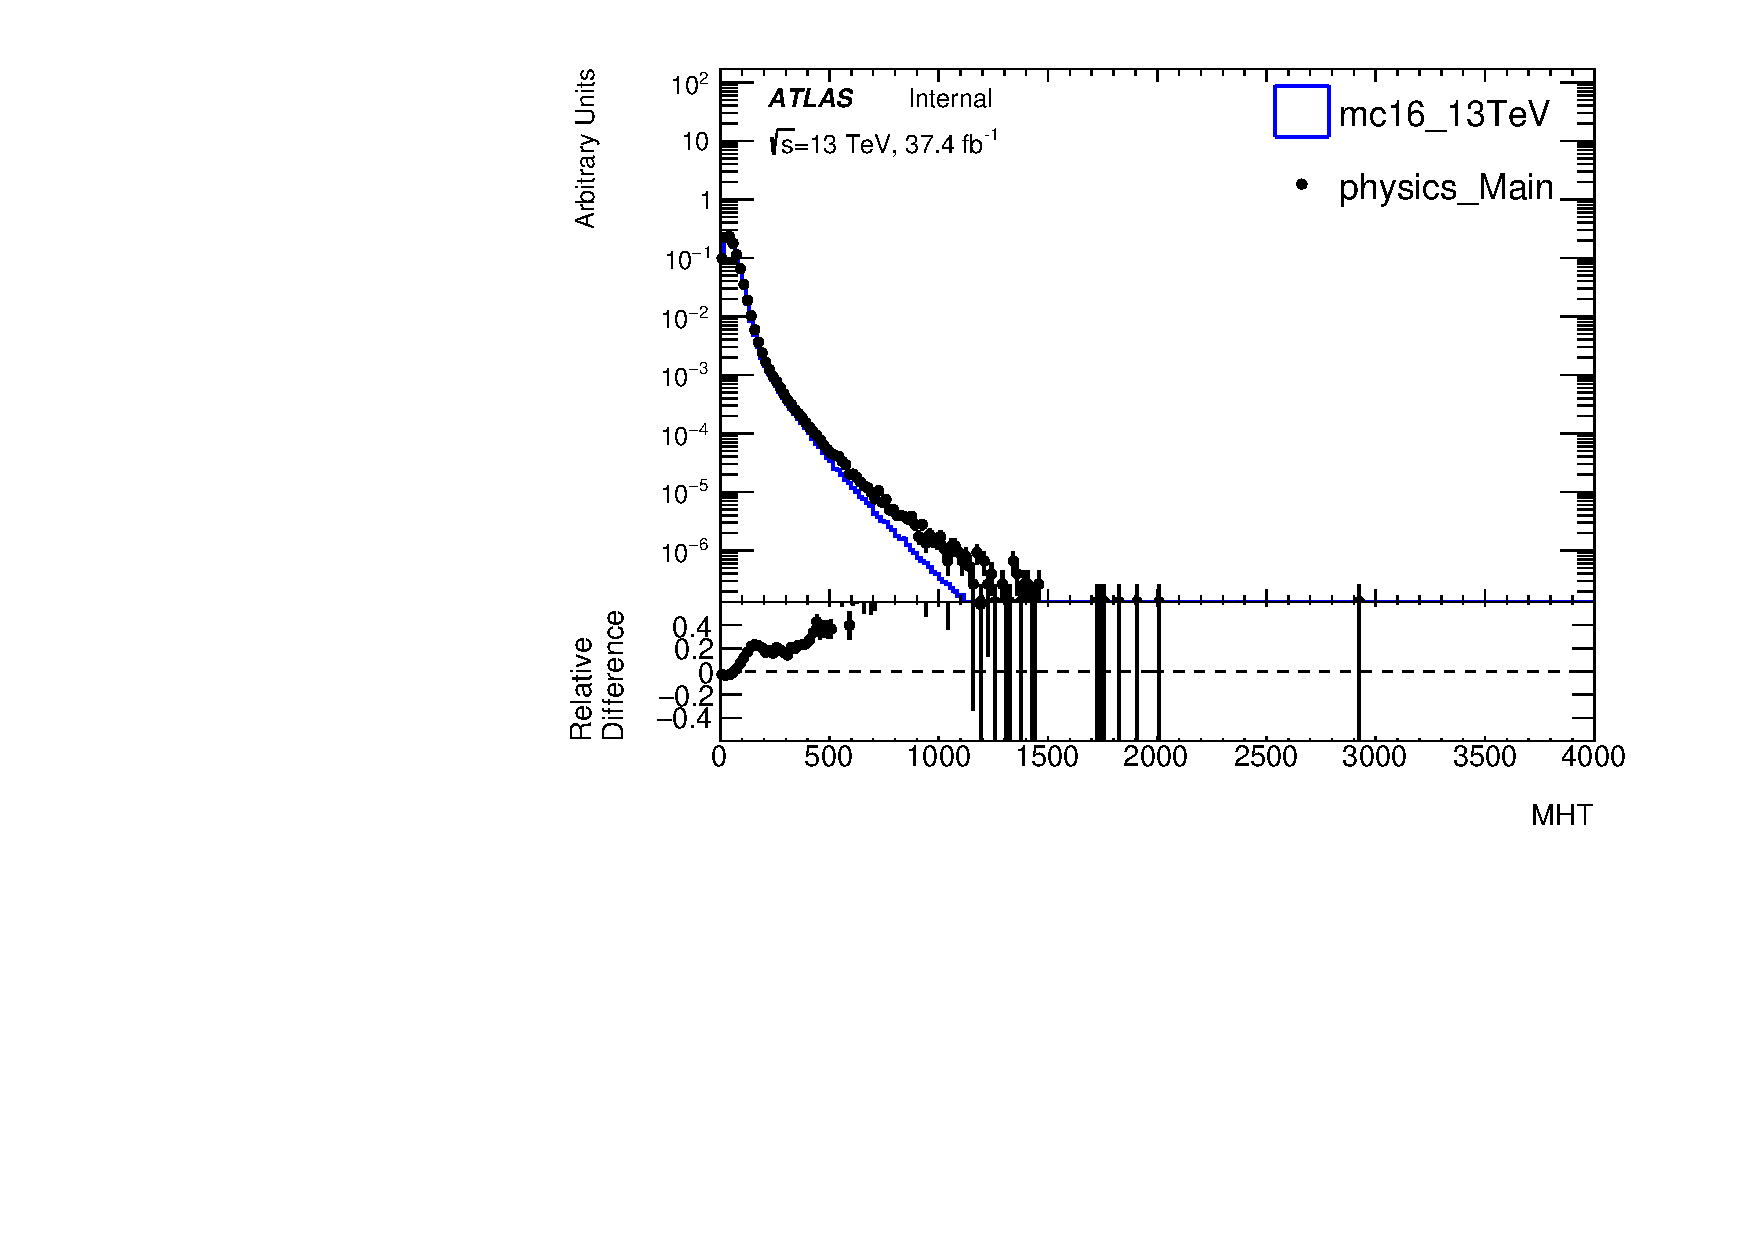
\includegraphics[width=0.45\textwidth]{figures/monitoring/resonant/2015-16/JJ/newStudy_MHT_logY_JJv01.pdf}}
% %
% \subfigure[] {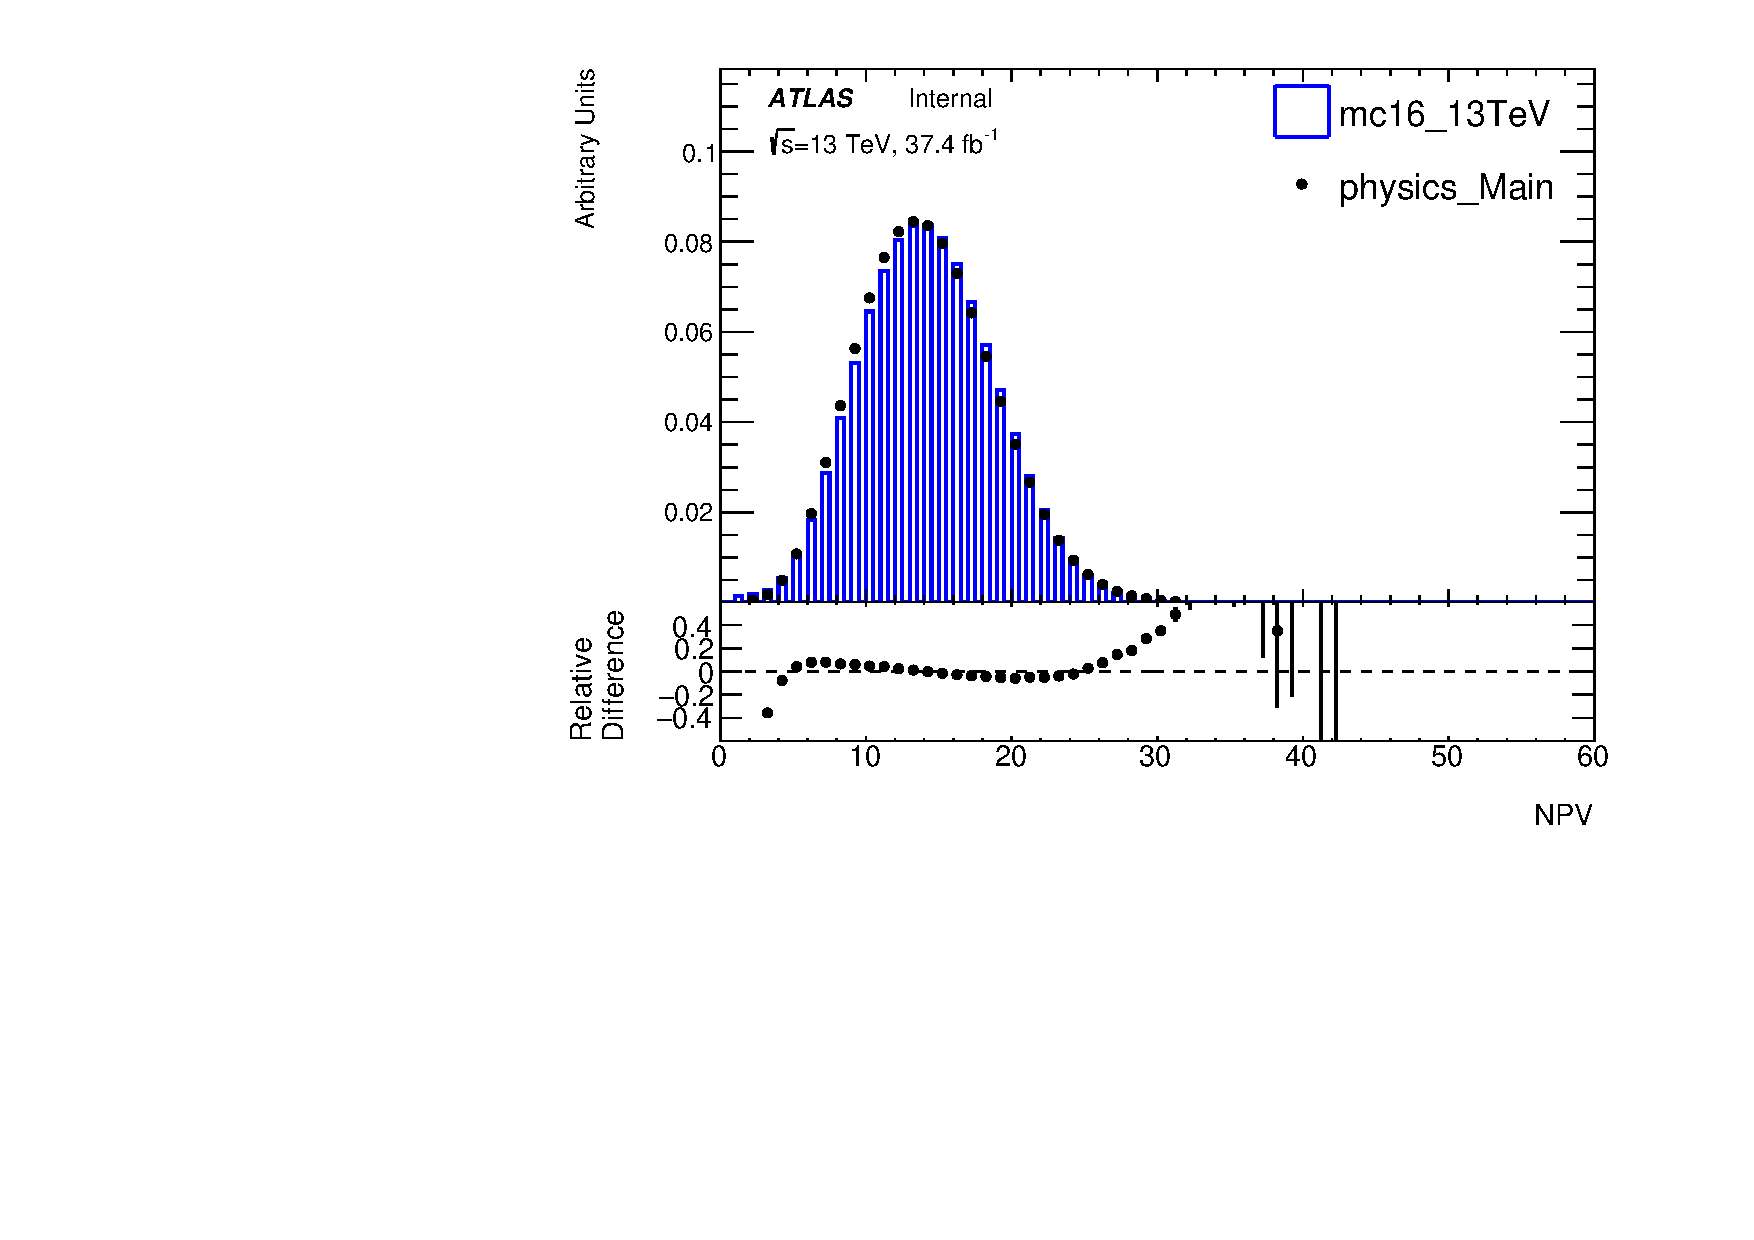
\includegraphics[width=0.45\textwidth]{figures/monitoring/resonant/2015-16/JJ/newStudy_NPV_JJv01.pdf}}
% \subfigure[] {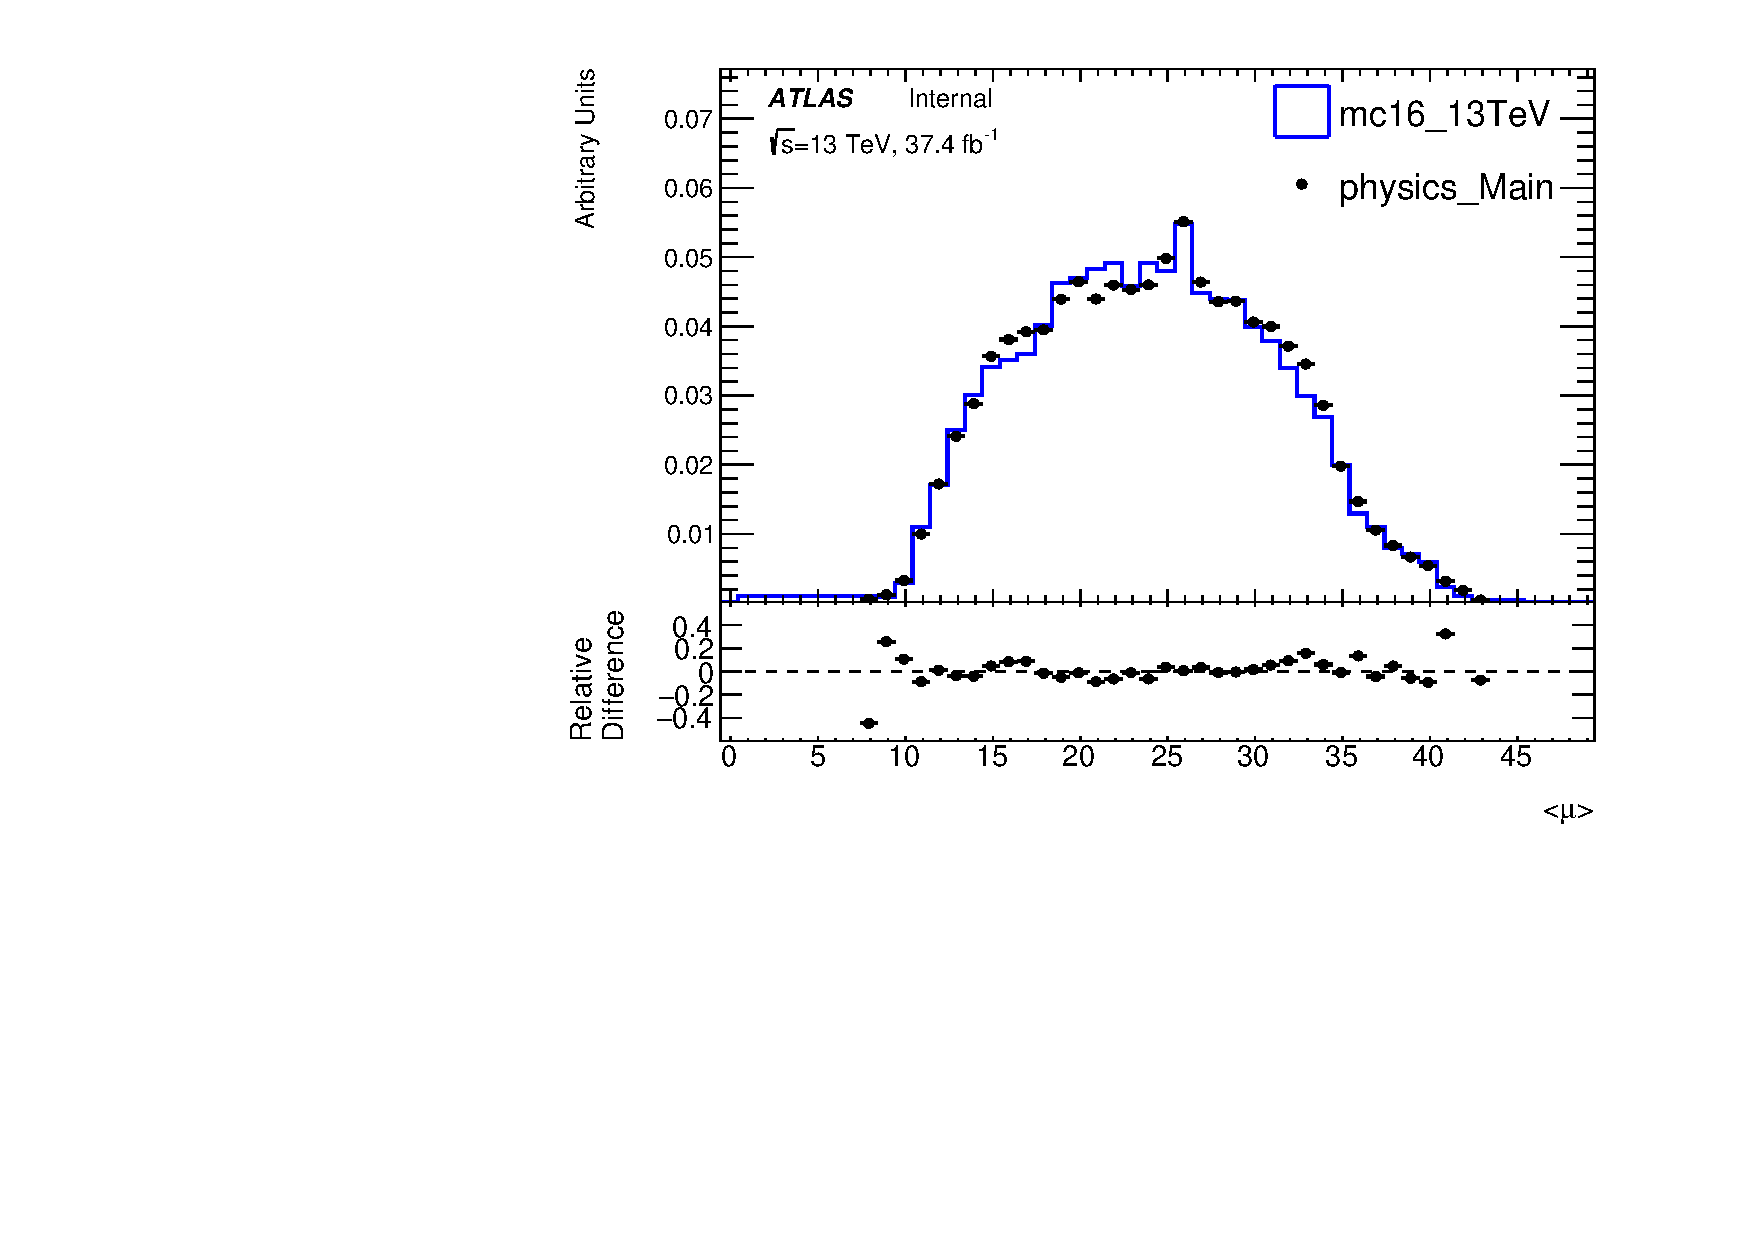
\includegraphics[width=0.45\textwidth]{figures/monitoring/resonant/2015-16/JJ/newStudy_averageInteractionsPerCrossing_JJv01.pdf}}
% %
%
% \caption{Monitoring plots on %2016 data, 
% the JJ resonant selection. (a) $H_T$, (b) $MH_T$ (missing transverse momentum calculated only from the jets in the event), (c) number of primary interaction vertices and (d) average interactions per bunch crossing.}
% \label{fig:JJmonitoring1}
%\end{figure}
%
% \begin{figure}[htb]
% \centering
%  %
% \subfigure[] {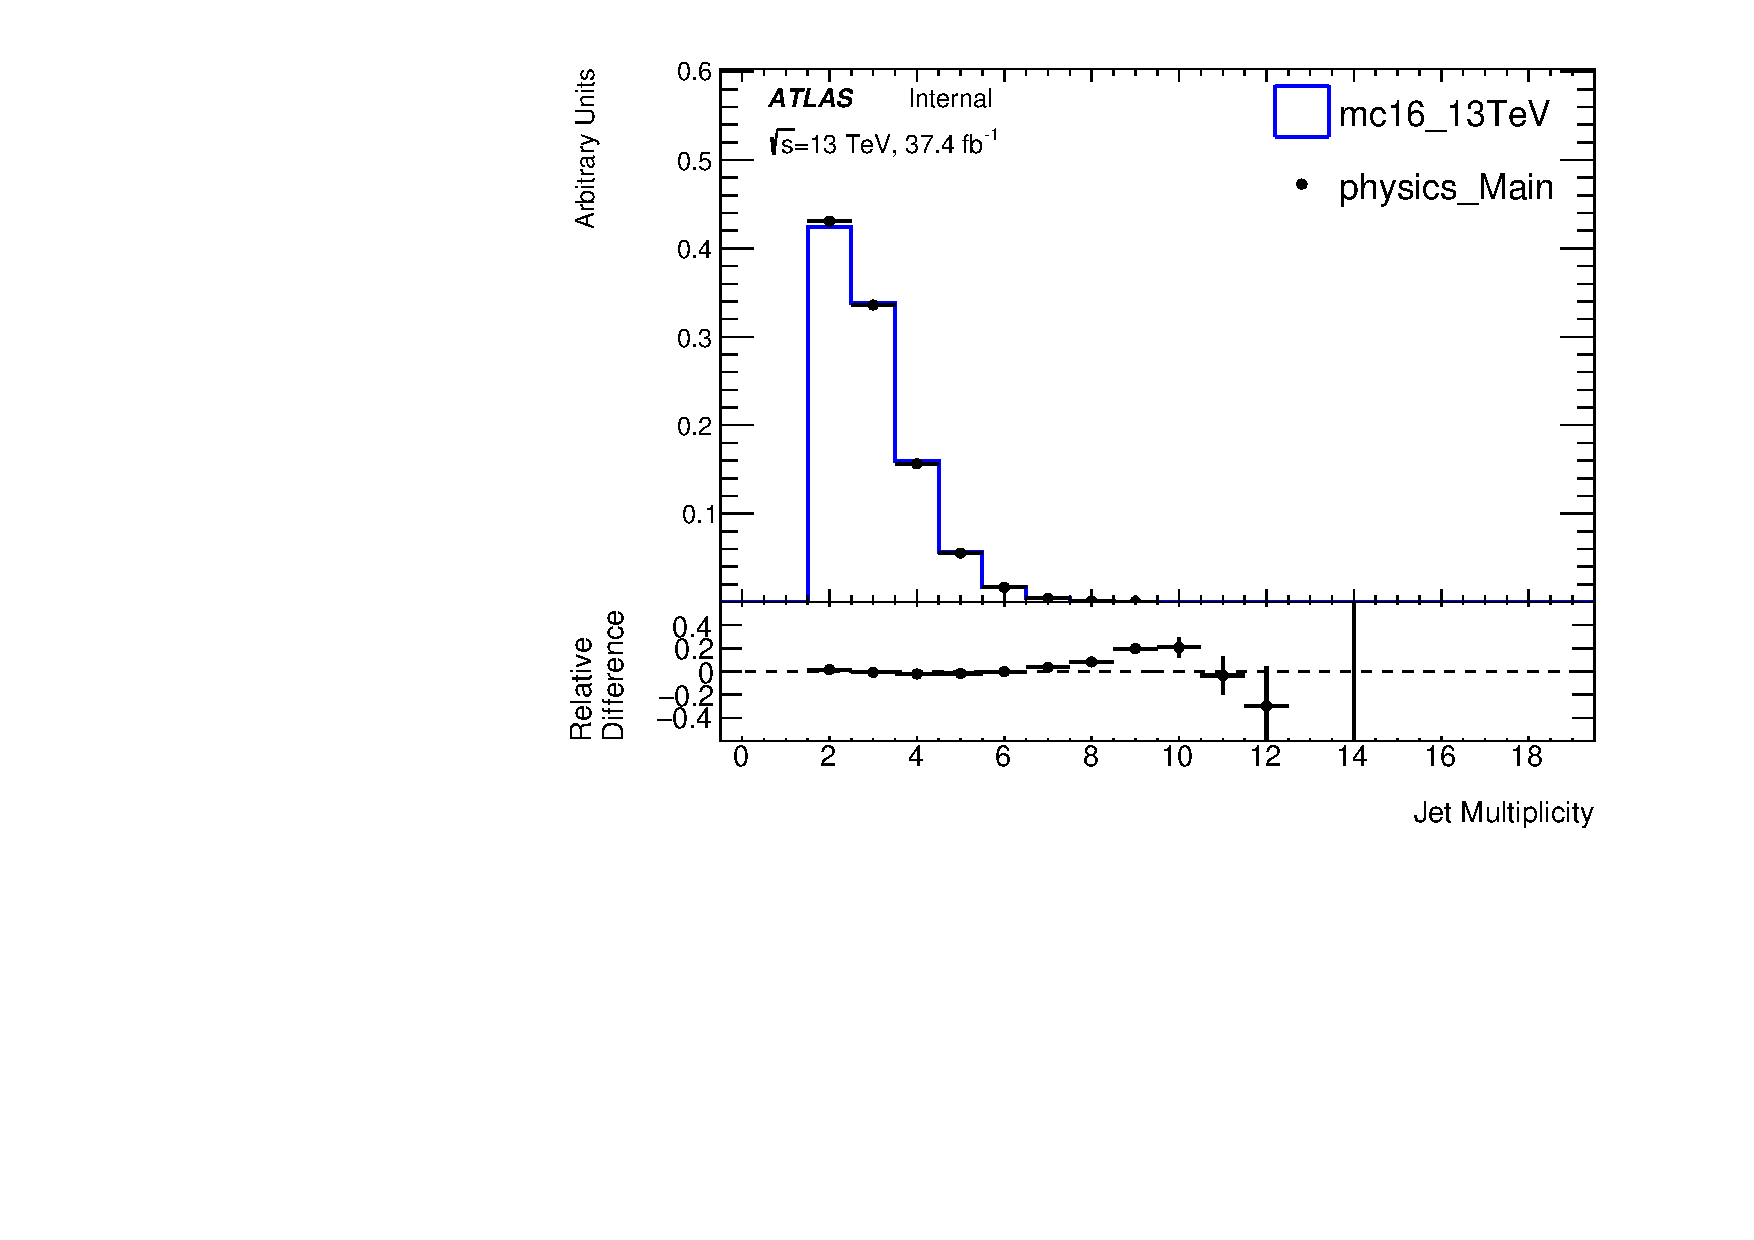
\includegraphics[width=0.45\textwidth]{figures/monitoring/resonant/2015-16/JJ/newStudy_njets_JJv01.pdf}}
% \subfigure[] {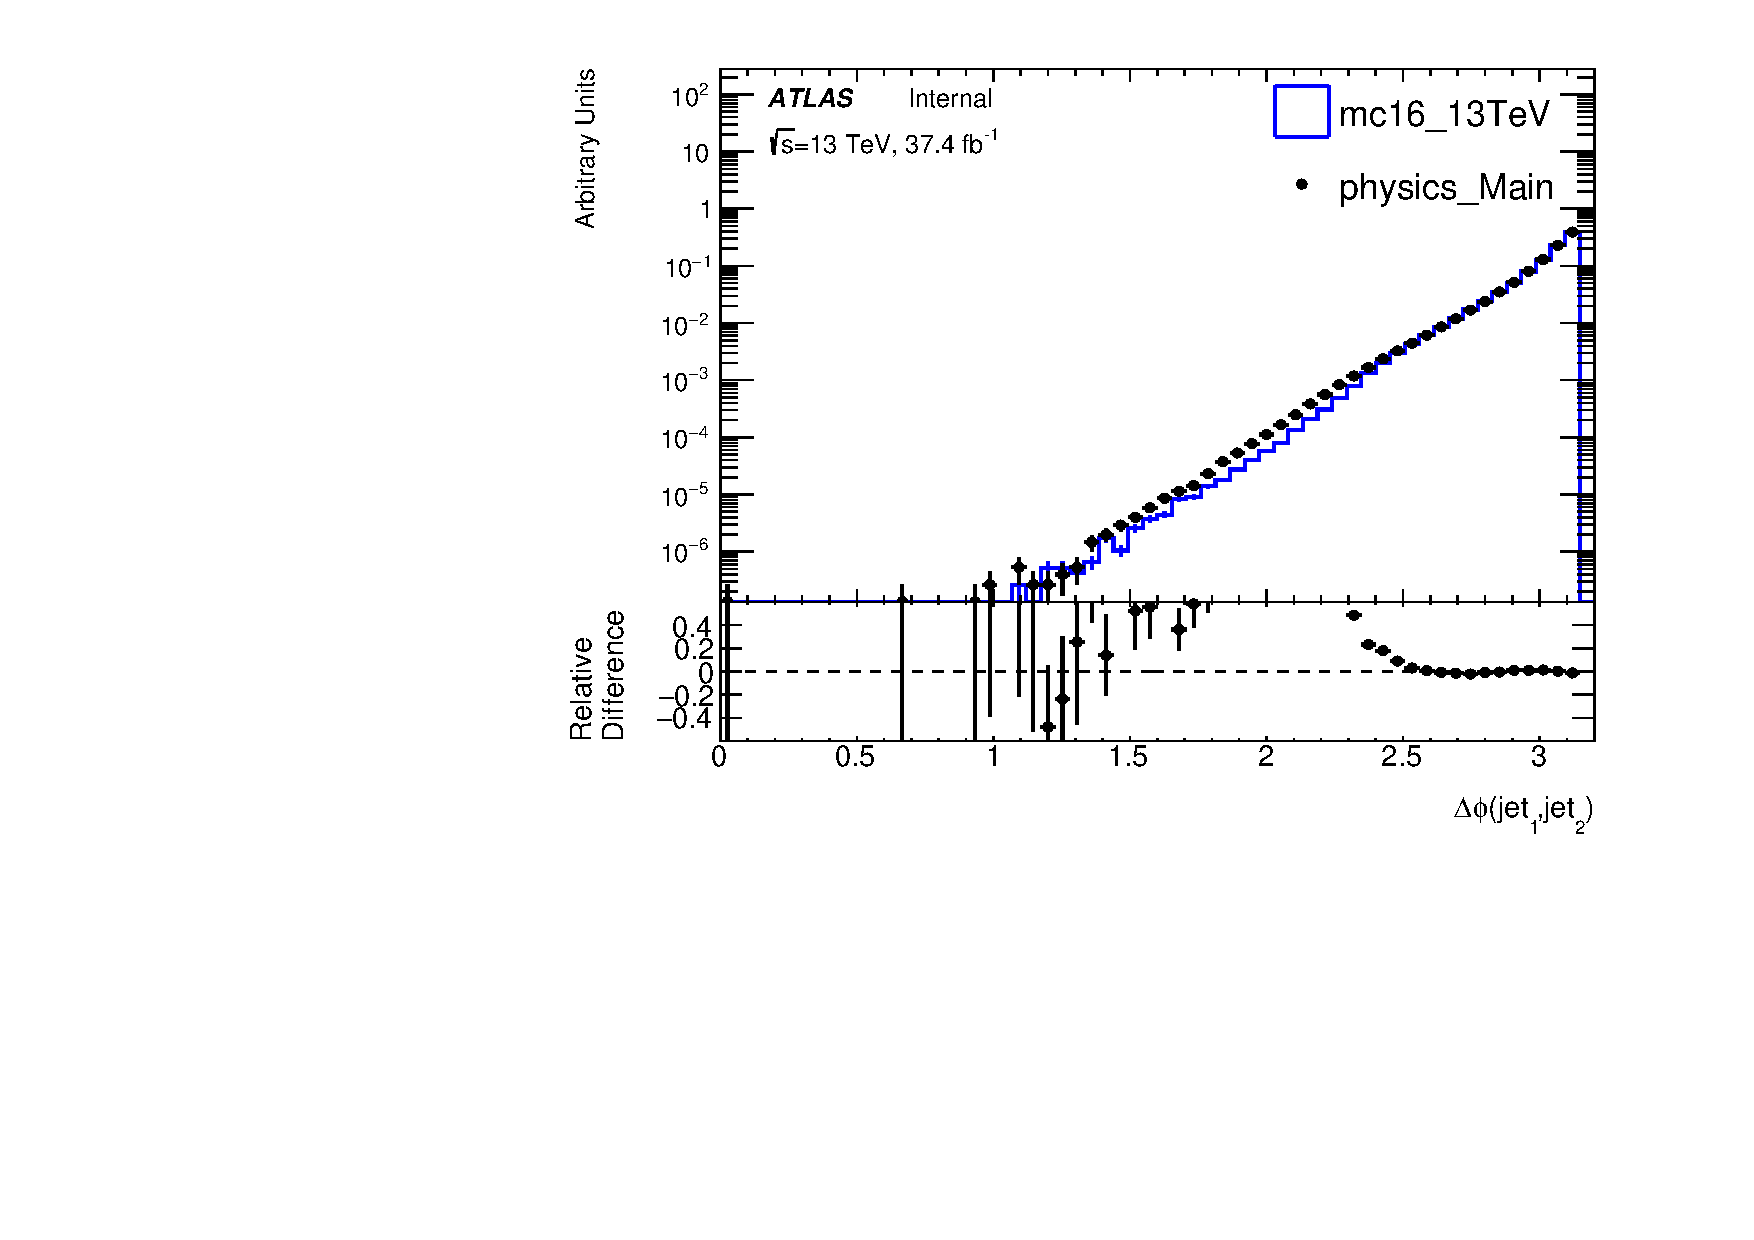
\includegraphics[width=0.45\textwidth]{figures/monitoring/resonant/2015-16/JJ//newStudy_deltaPhi_logY_JJv01.pdf}}
%
%%
% \subfigure[] {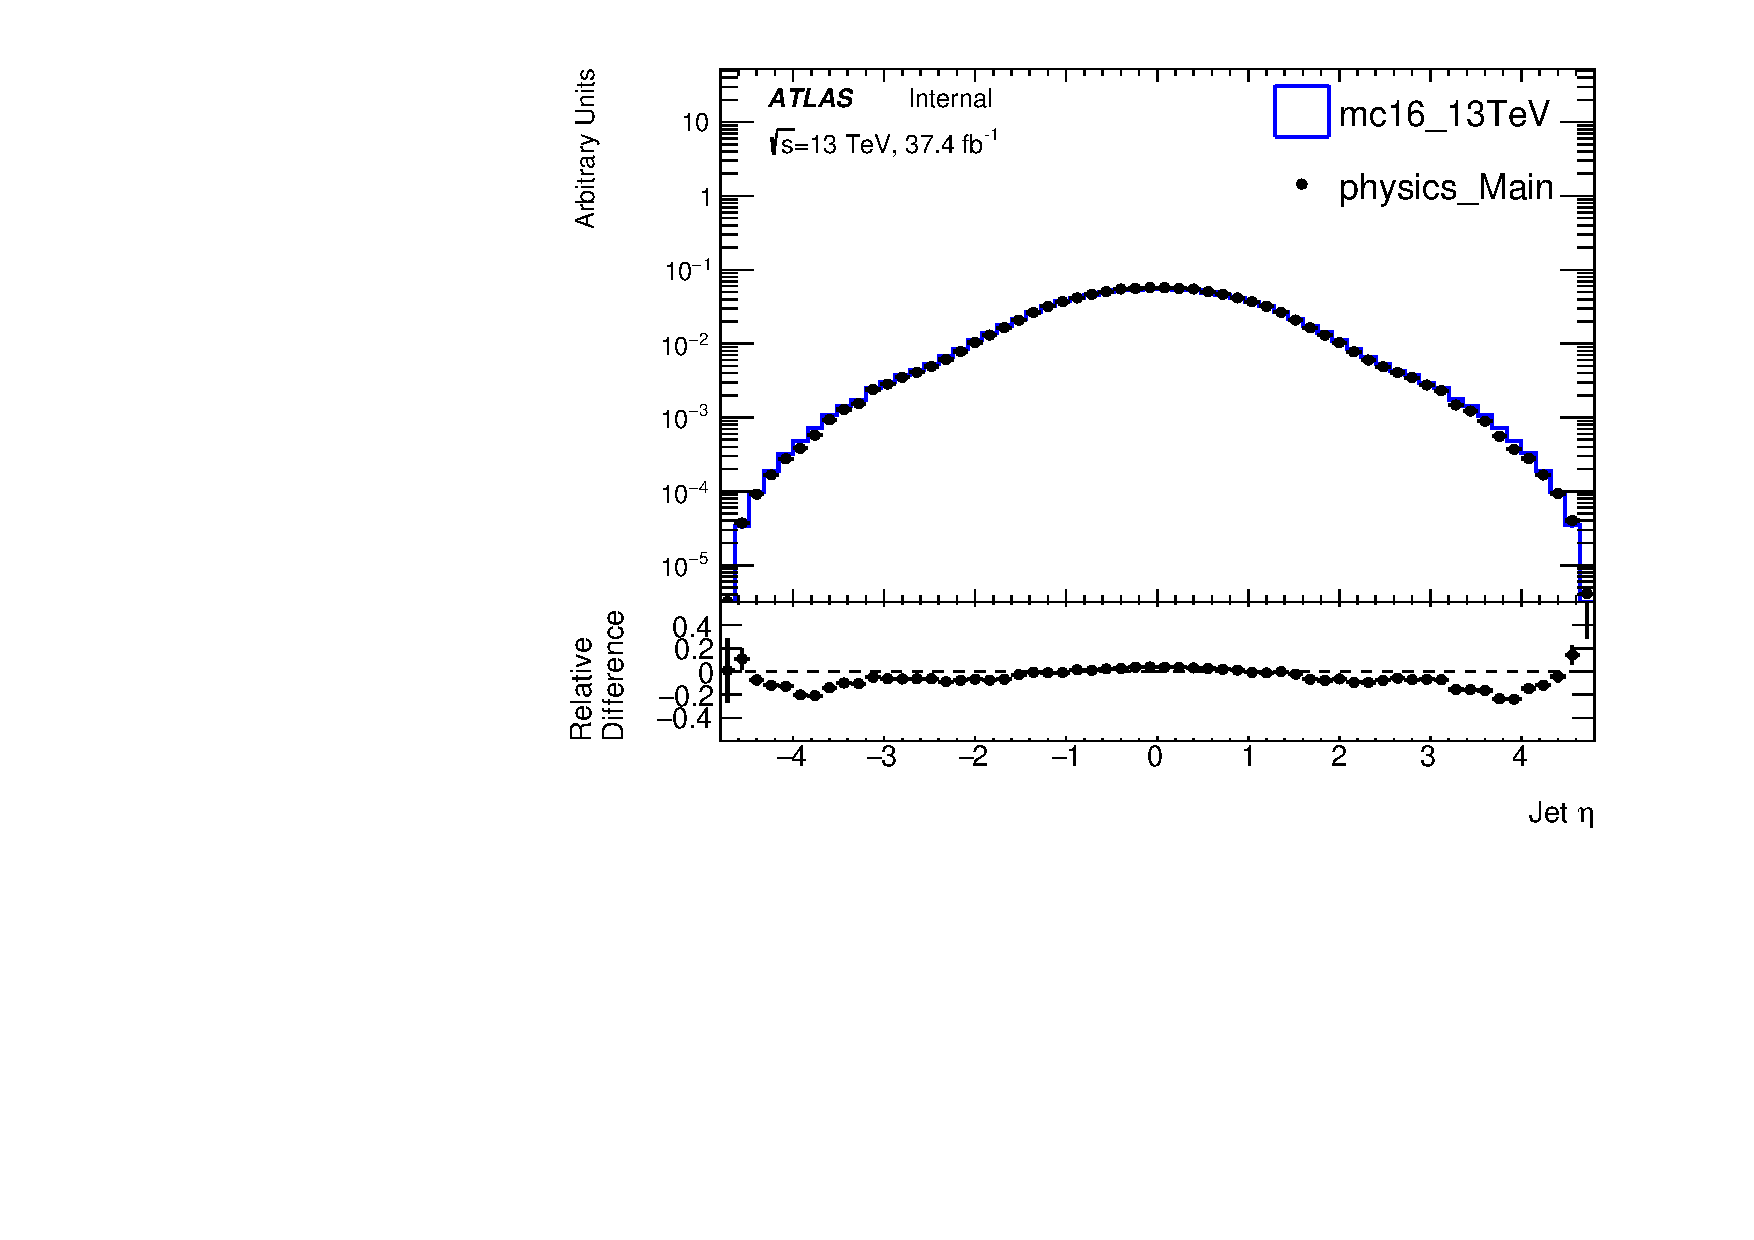
\includegraphics[width=0.45\textwidth]{figures/monitoring/resonant/2015-16/JJ/newStudy_jet_eta_logY_JJv01.pdf}}
% \subfigure[] {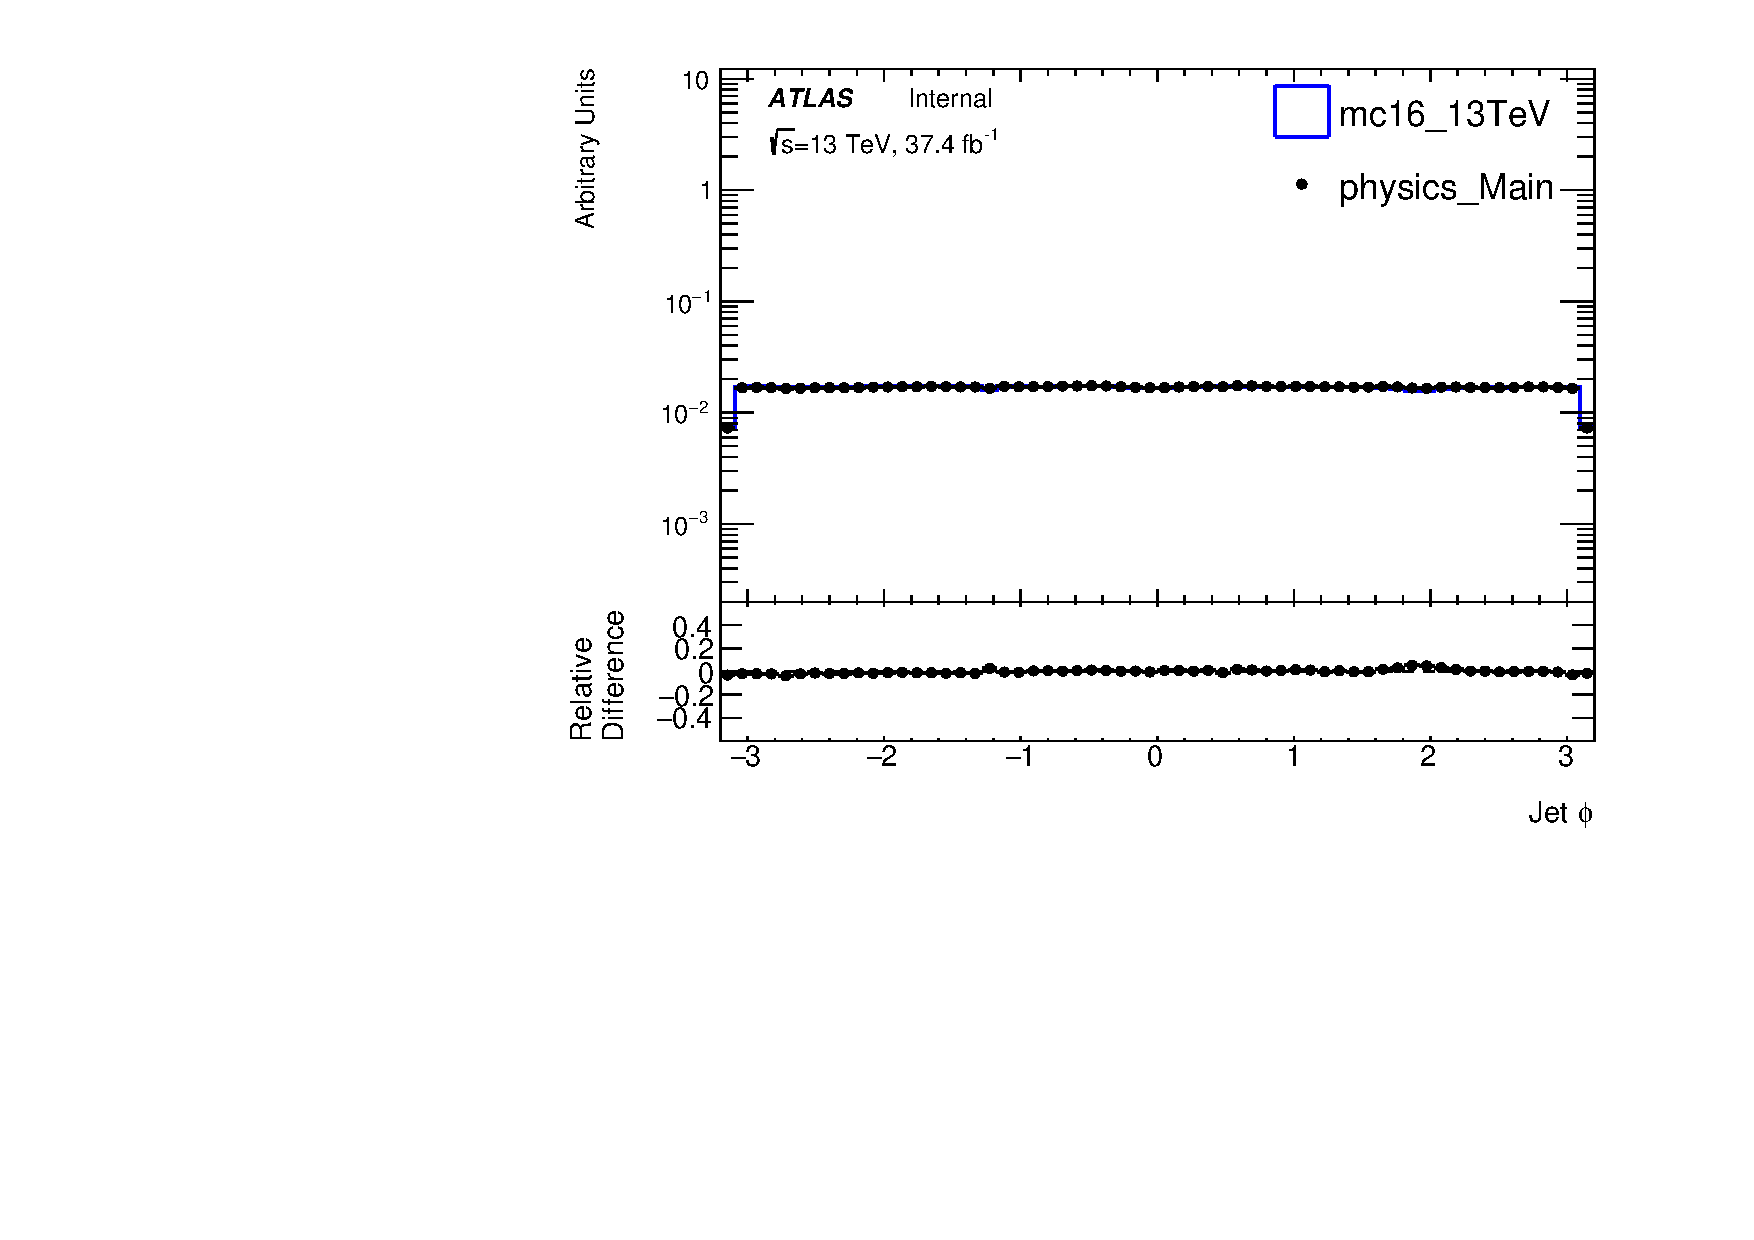
\includegraphics[width=0.45\textwidth]{figures/monitoring/resonant/2015-16/JJ/newStudy_jet_phi_logY_JJv01.pdf}}
% %
% \subfigure[] {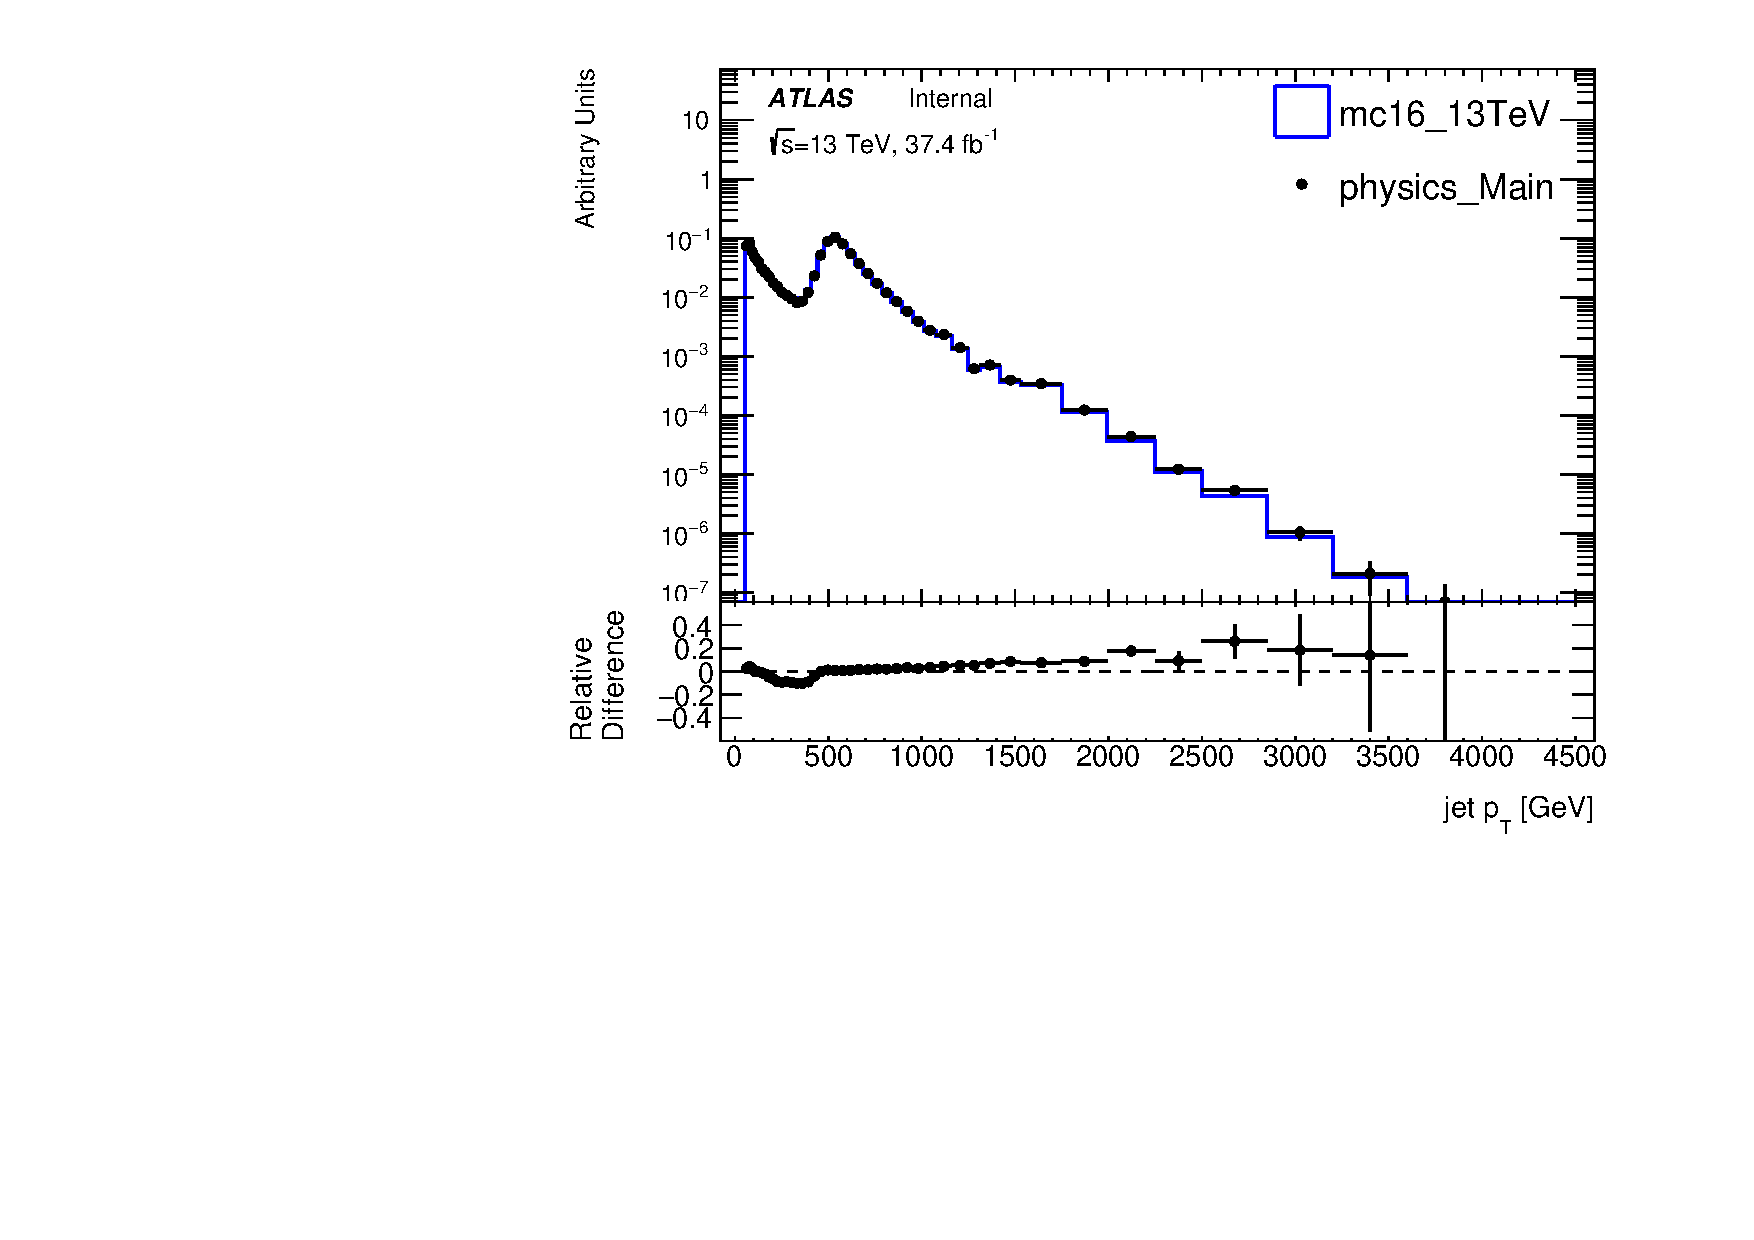
\includegraphics[width=0.45\textwidth]{figures/monitoring/resonant/2015-16/JJ/newStudy_jet_pt_logY_JJv01.pdf}}
% \subfigure[] {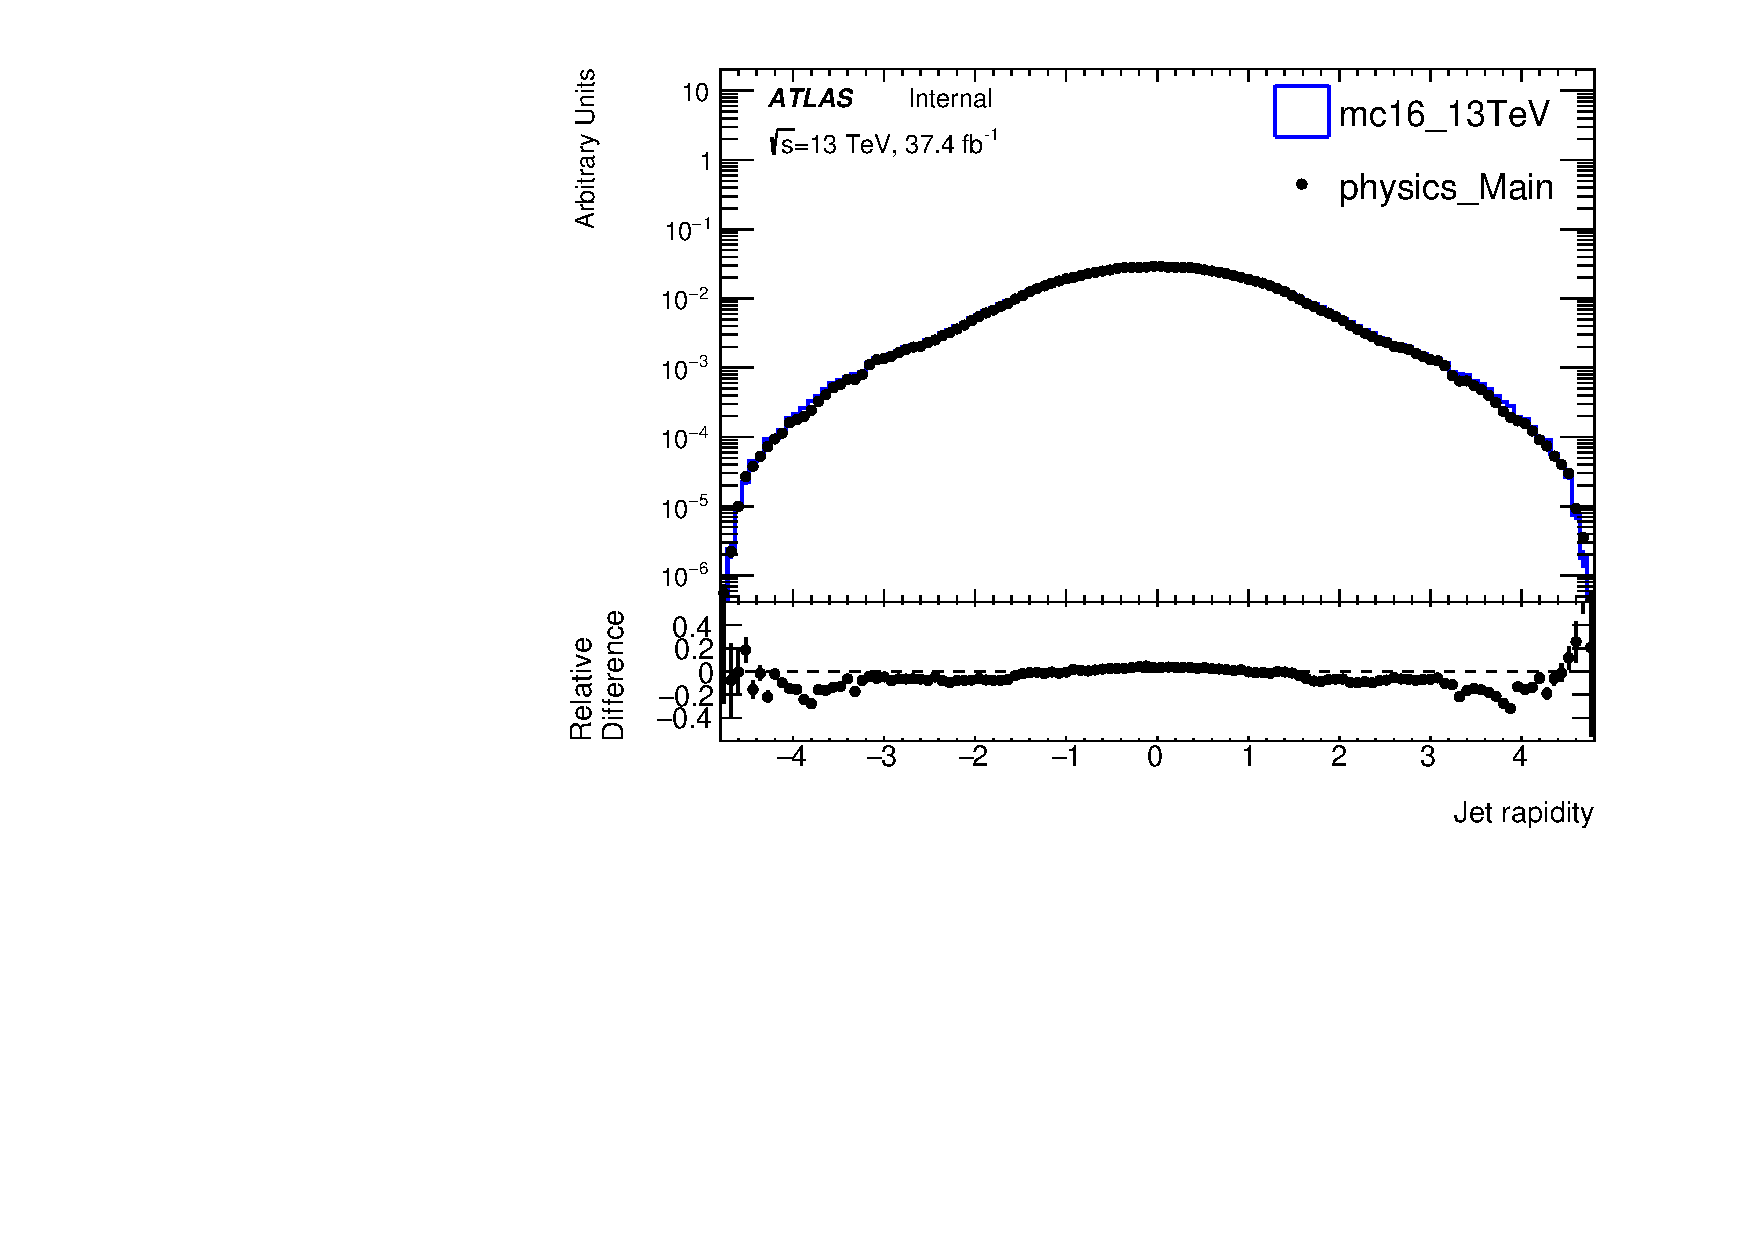
\includegraphics[width=0.45\textwidth]{figures/monitoring/resonant/2015-16/JJ/newStudy_jet_rapidity_logY_JJv01.pdf}}
% %
% 
%  \caption{Jet plots on %2016 data, 
%  the resonant selection. (a) number of jets (b) $\Delta\phi$ between the two jets (c) jet $\eta$
%  (d) jet $\phi$ (e) jet \pT\ (f) jet rapidity.  Fluctuations in the jet $phi$ distribution are attributable to dead modules in the tile calorimeter which lead to fewer jets in small slices of the detector.}
% \label{fig:JJmonitoring5}
%\end{figure}
%
%
% \begin{figure}[htb]
% \centering
% %
% \subfigure[] {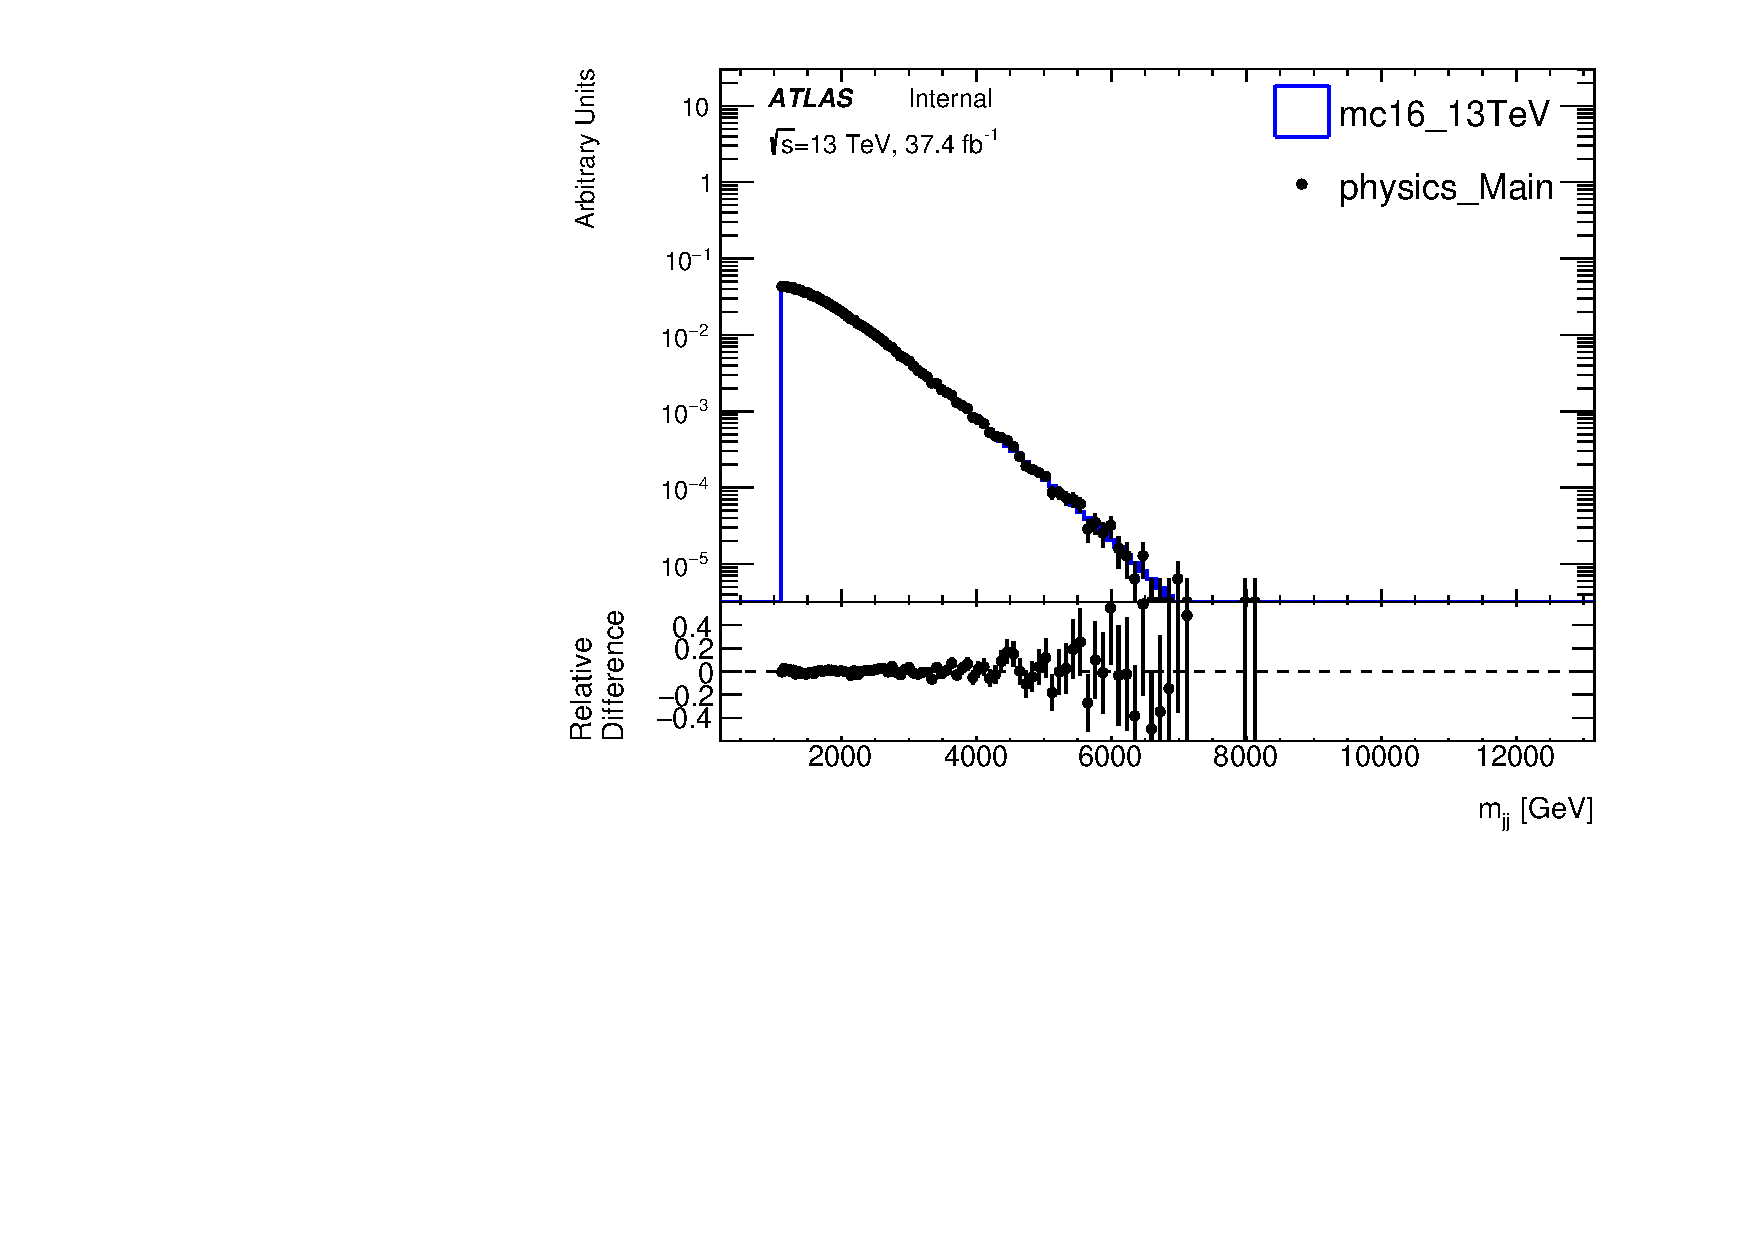
\includegraphics[width=0.45\textwidth]{figures/monitoring/resonant/2015-16/QQ/newStudy_mjj_logY_QQv01.pdf}}
% \subfigure[] {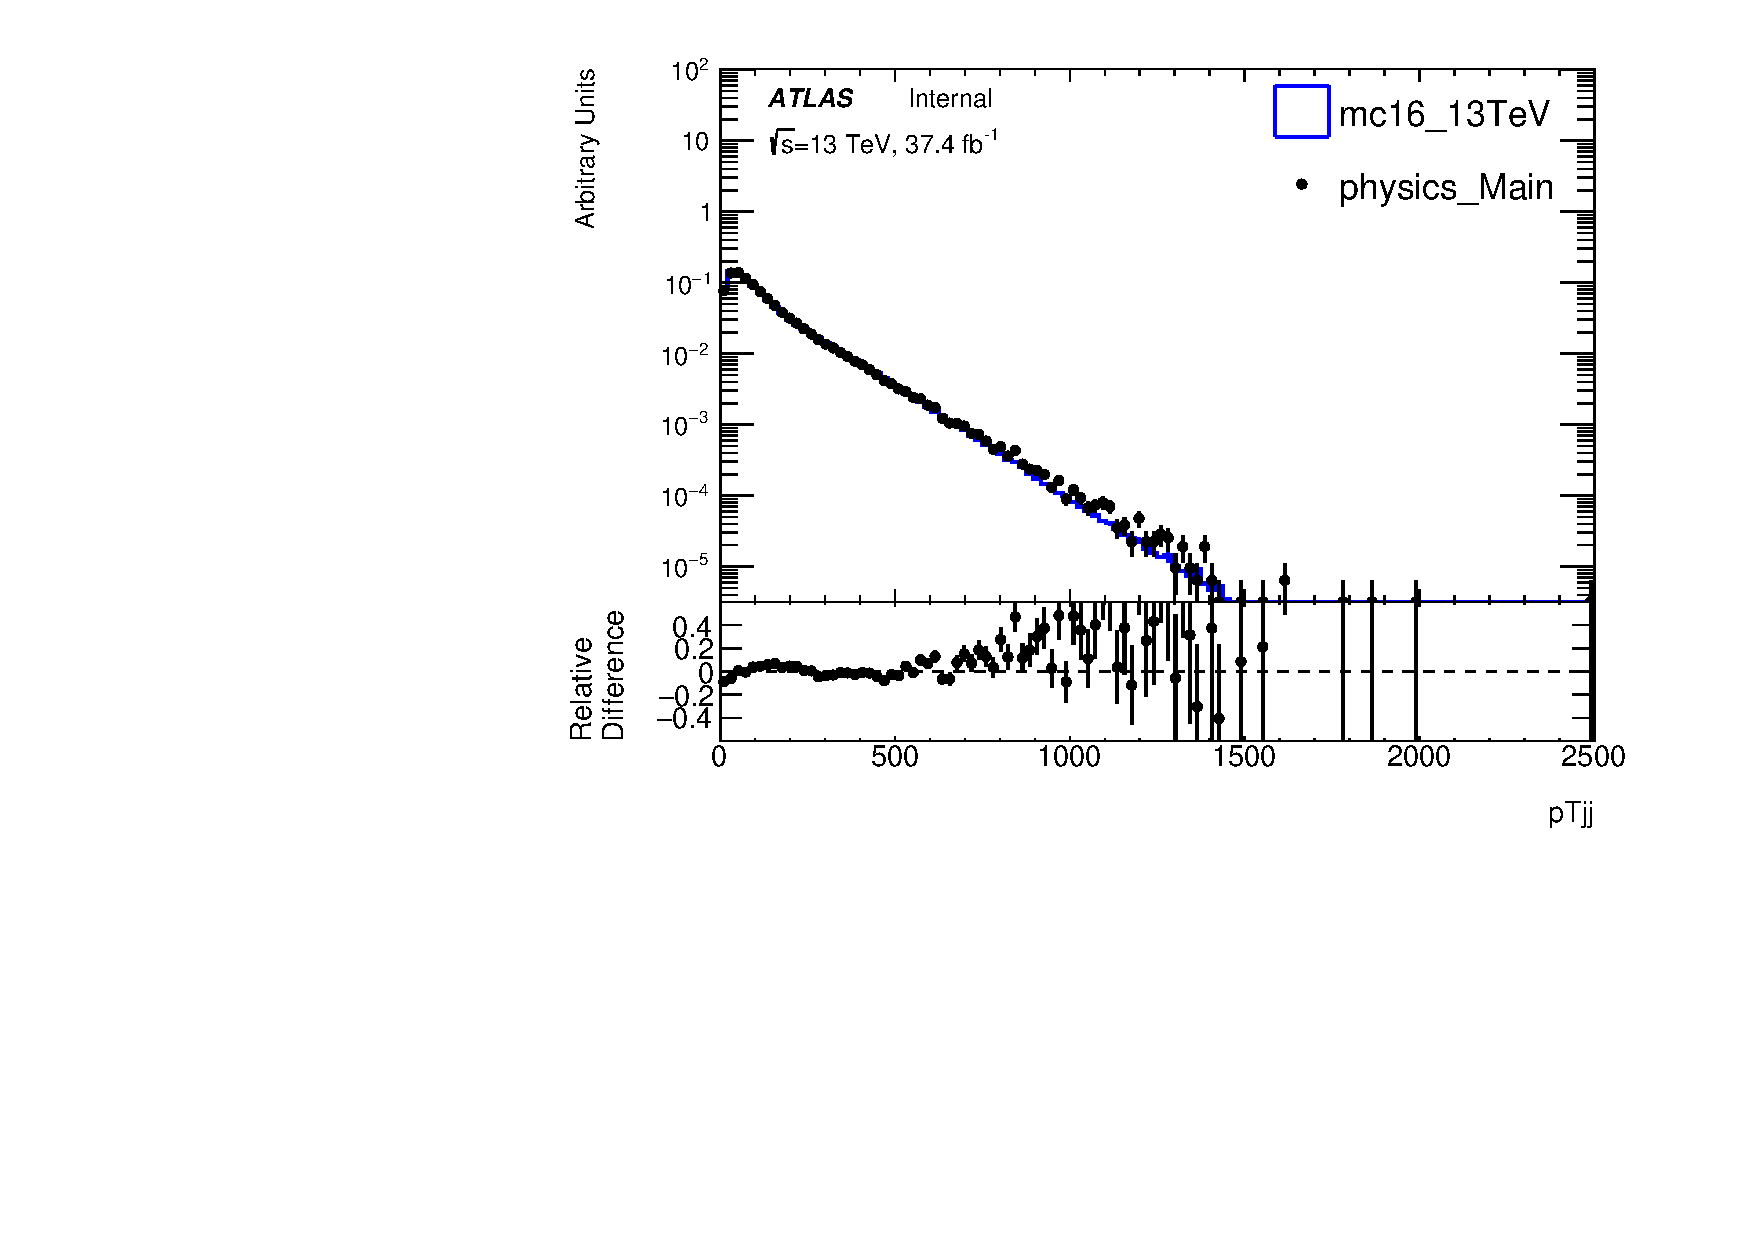
\includegraphics[width=0.45\textwidth]{figures/monitoring/resonant/2015-16/QQ/newStudy_pTjj_logY_QQv01.pdf}}
% %
% \subfigure[] {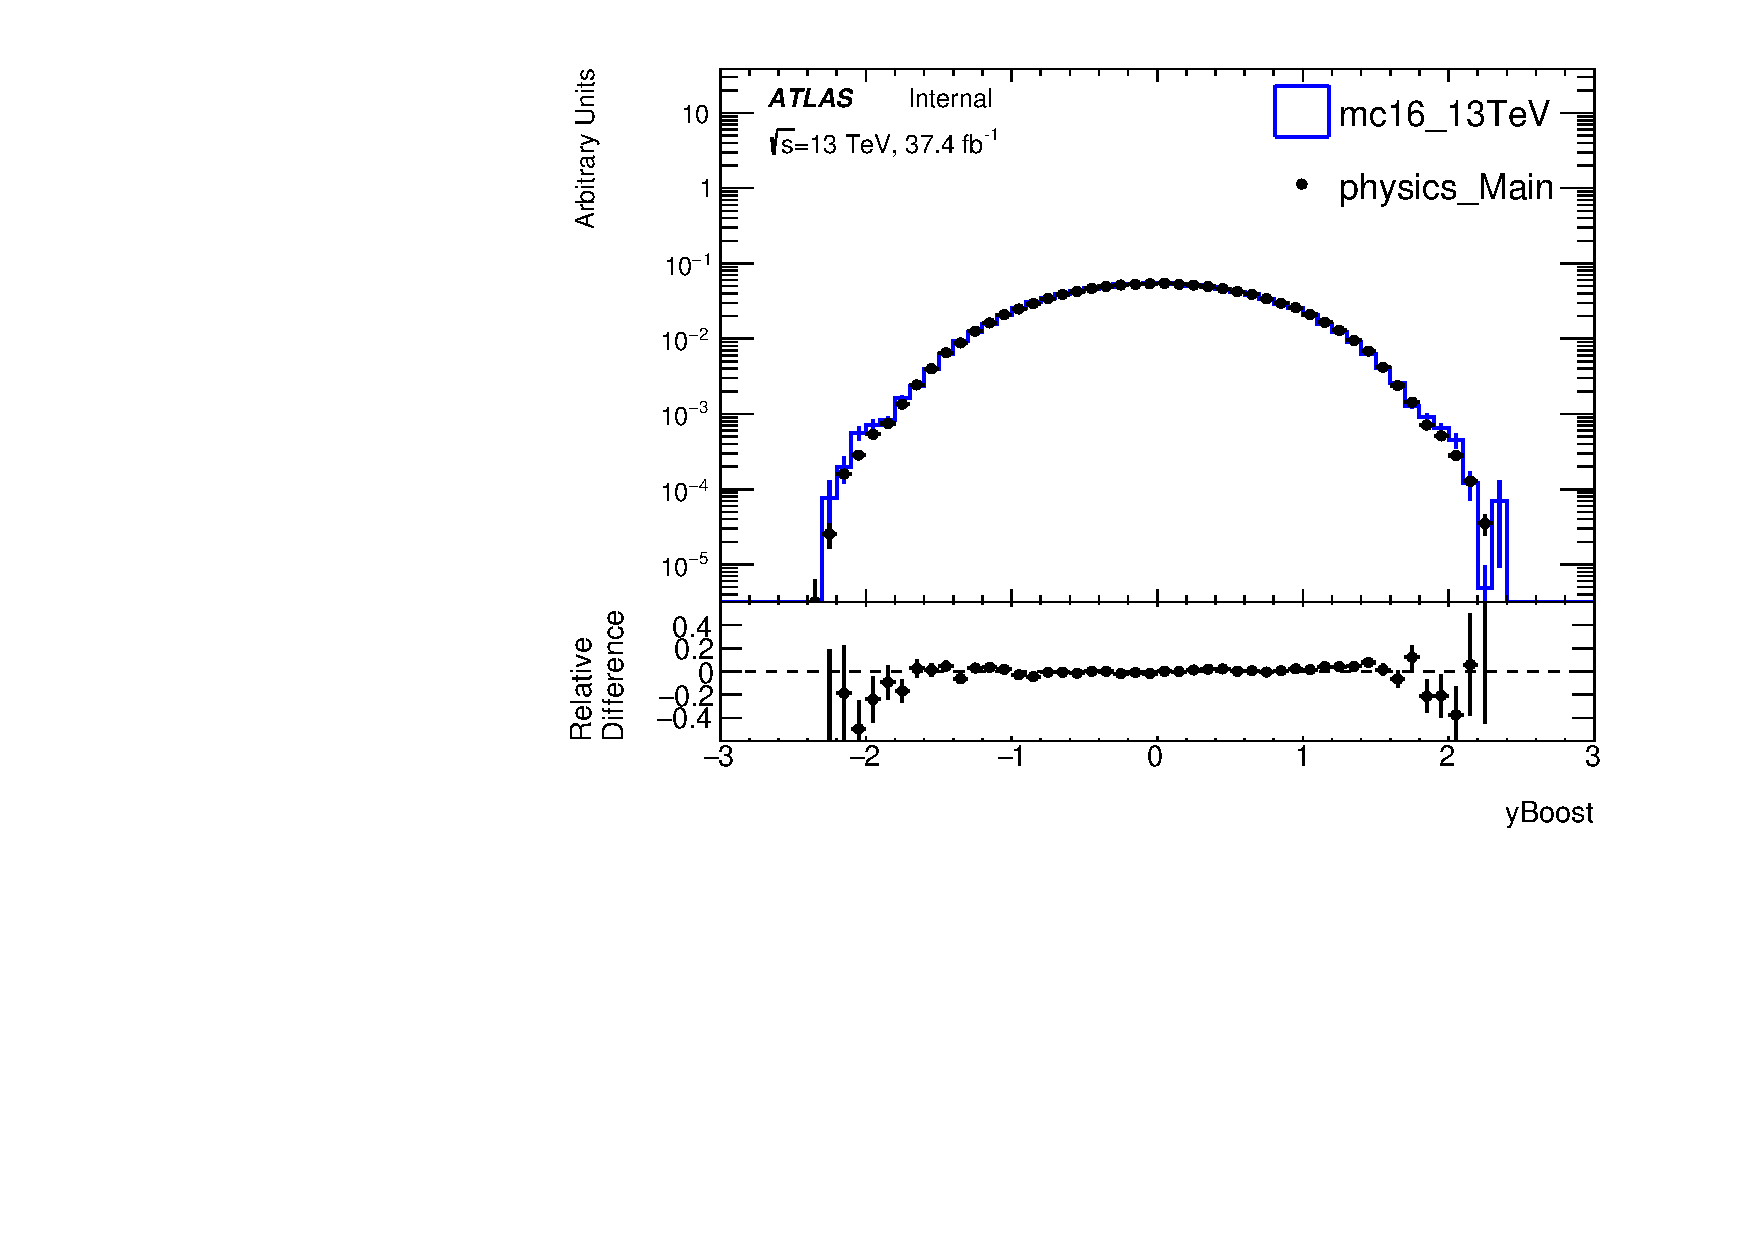
\includegraphics[width=0.45\textwidth]{figures/monitoring/resonant/2015-16/QQ/newStudy_yBoost_logY_QQv01.pdf}}
% \subfigure[] {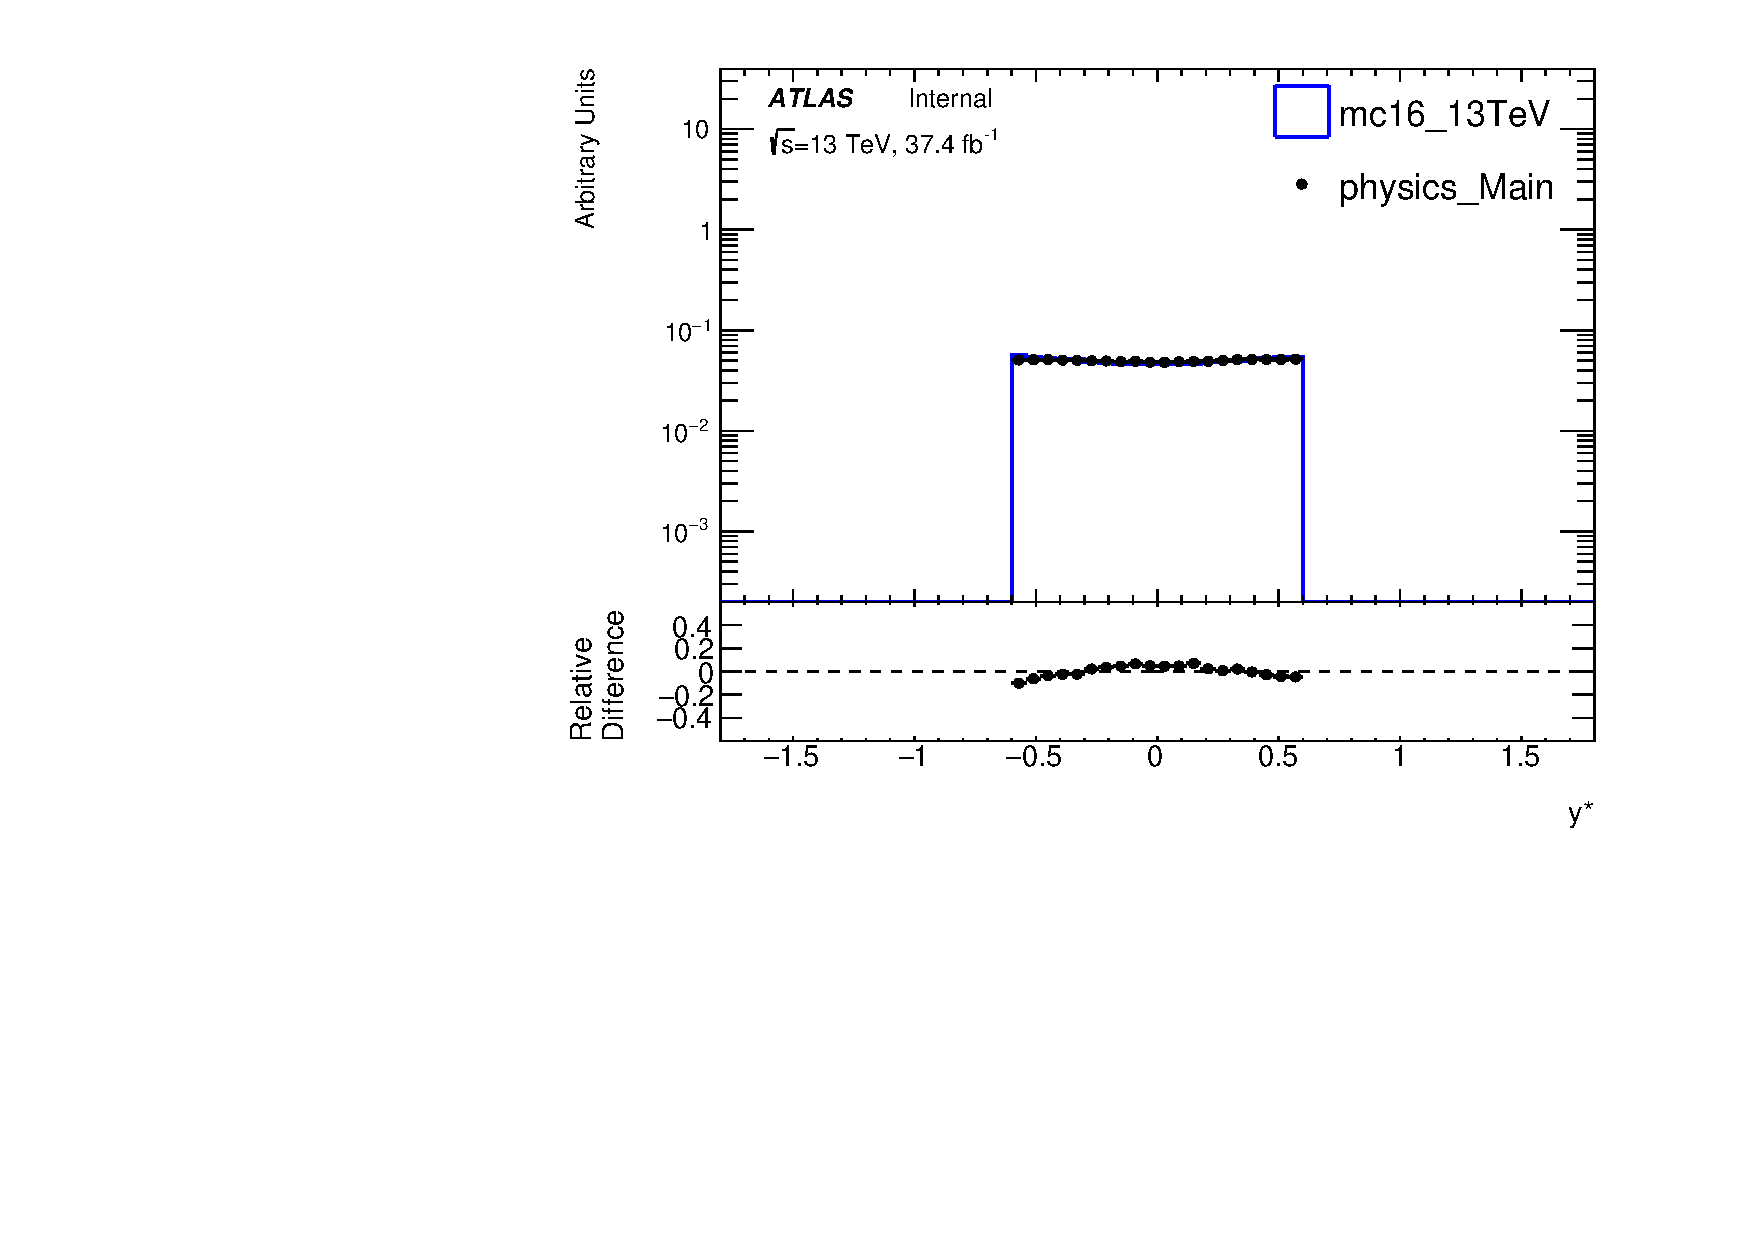
\includegraphics[width=0.45\textwidth]{figures/monitoring/resonant/2015-16/QQ/newStudy_yStar_logY_QQv01.pdf}}
% \caption{Jet plots on %2016 data, 
% the resonant selection. (a) dijet invariant mass (b) dijet \pT\ (c) \yB{} (d) \ystar{}. }
% \label{fig:JJmonitoring6}
%\end{figure}
%
%
%\clearpage
%
%
%In this section a selection of kinematic and monitoring plots produced with the resonant selection on the QQ dataset is shown 
%(Figures~\ref{fig:QQmonitoring1},  
%\ref{fig:QQmonitoring5}, \ref{fig:QQmonitoring6}). These plots are relative to \integLumi of data collected in 2015 and 2016.
% GRL has been applied here.
%
%\begin{figure}[htb]
% \centering
% \subfigure[] {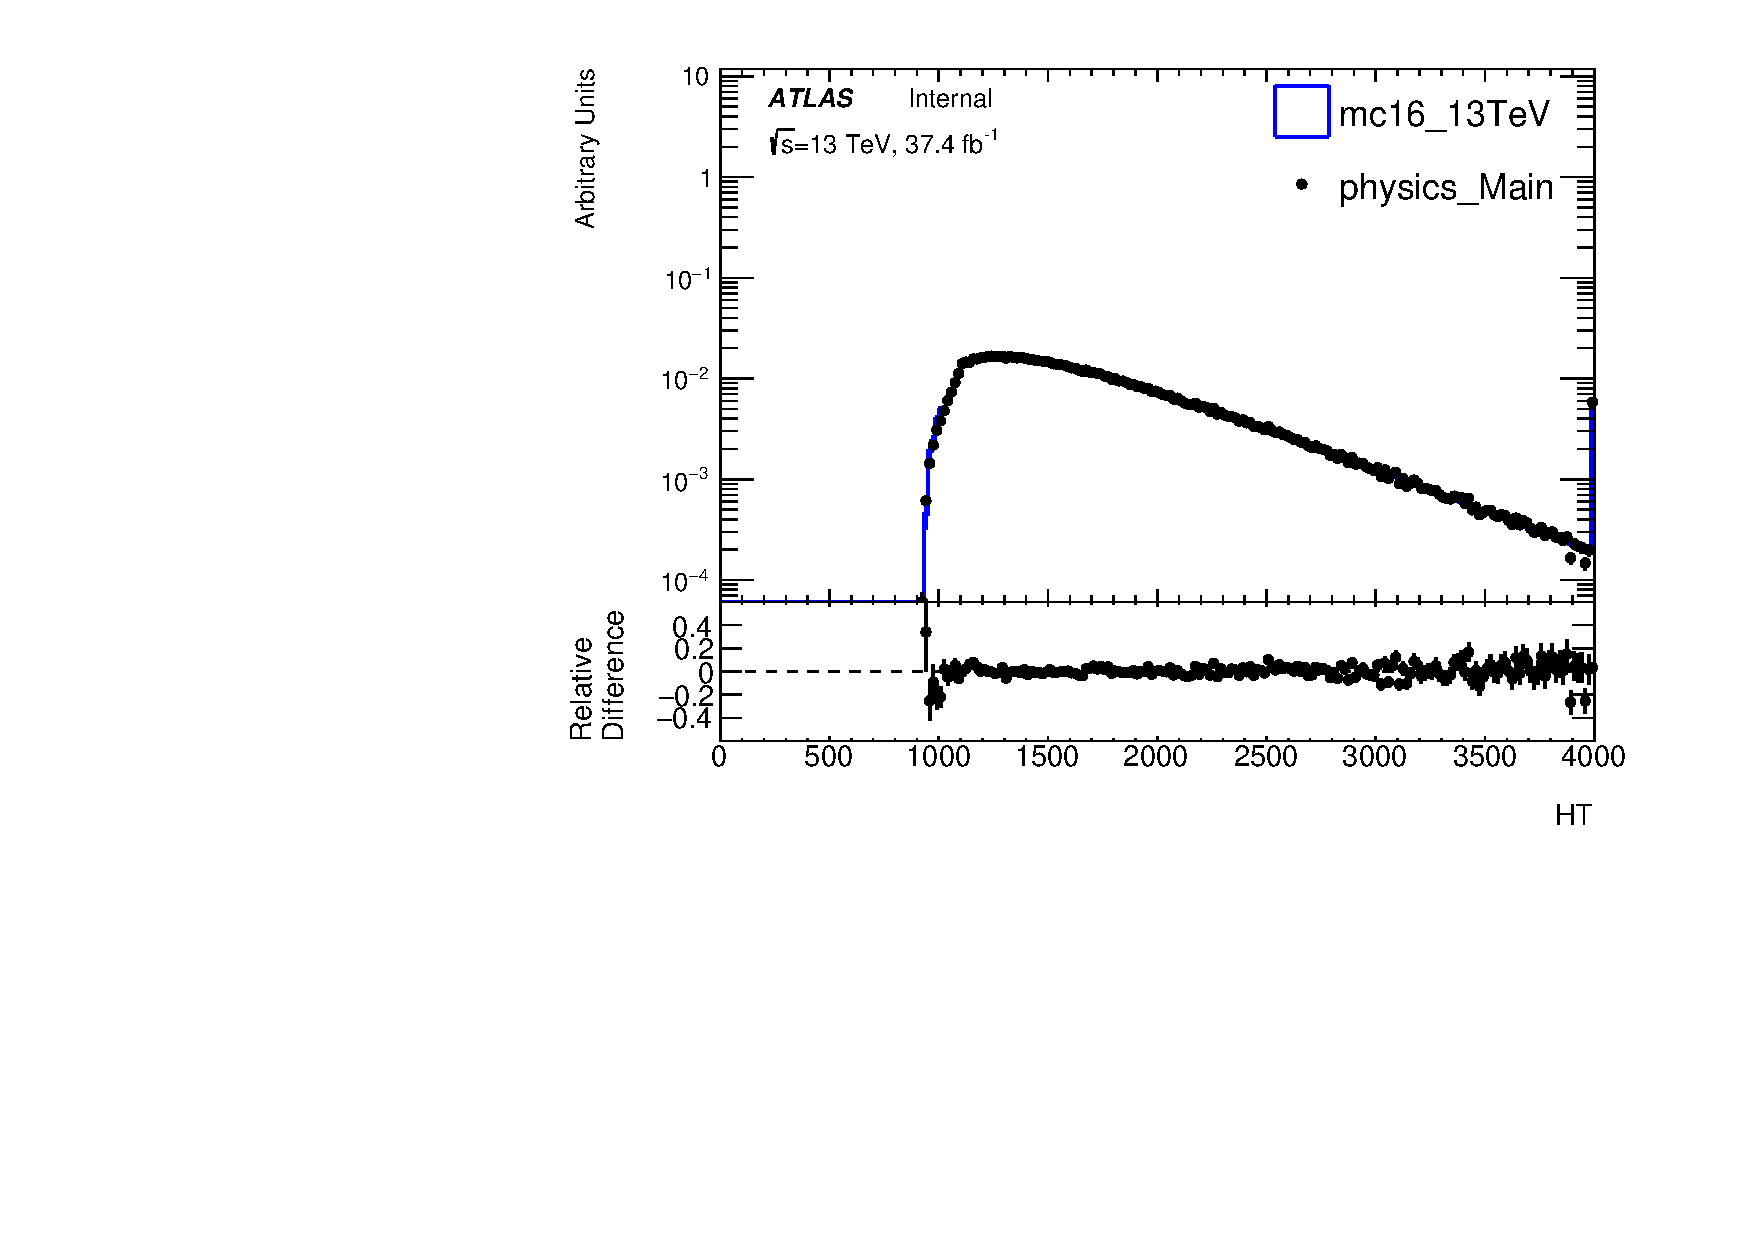
\includegraphics[width=0.45\textwidth]{figures/monitoring/resonant/2015-16/QQ/newStudy_HT_logY_QQv01.pdf}}
% \subfigure[] {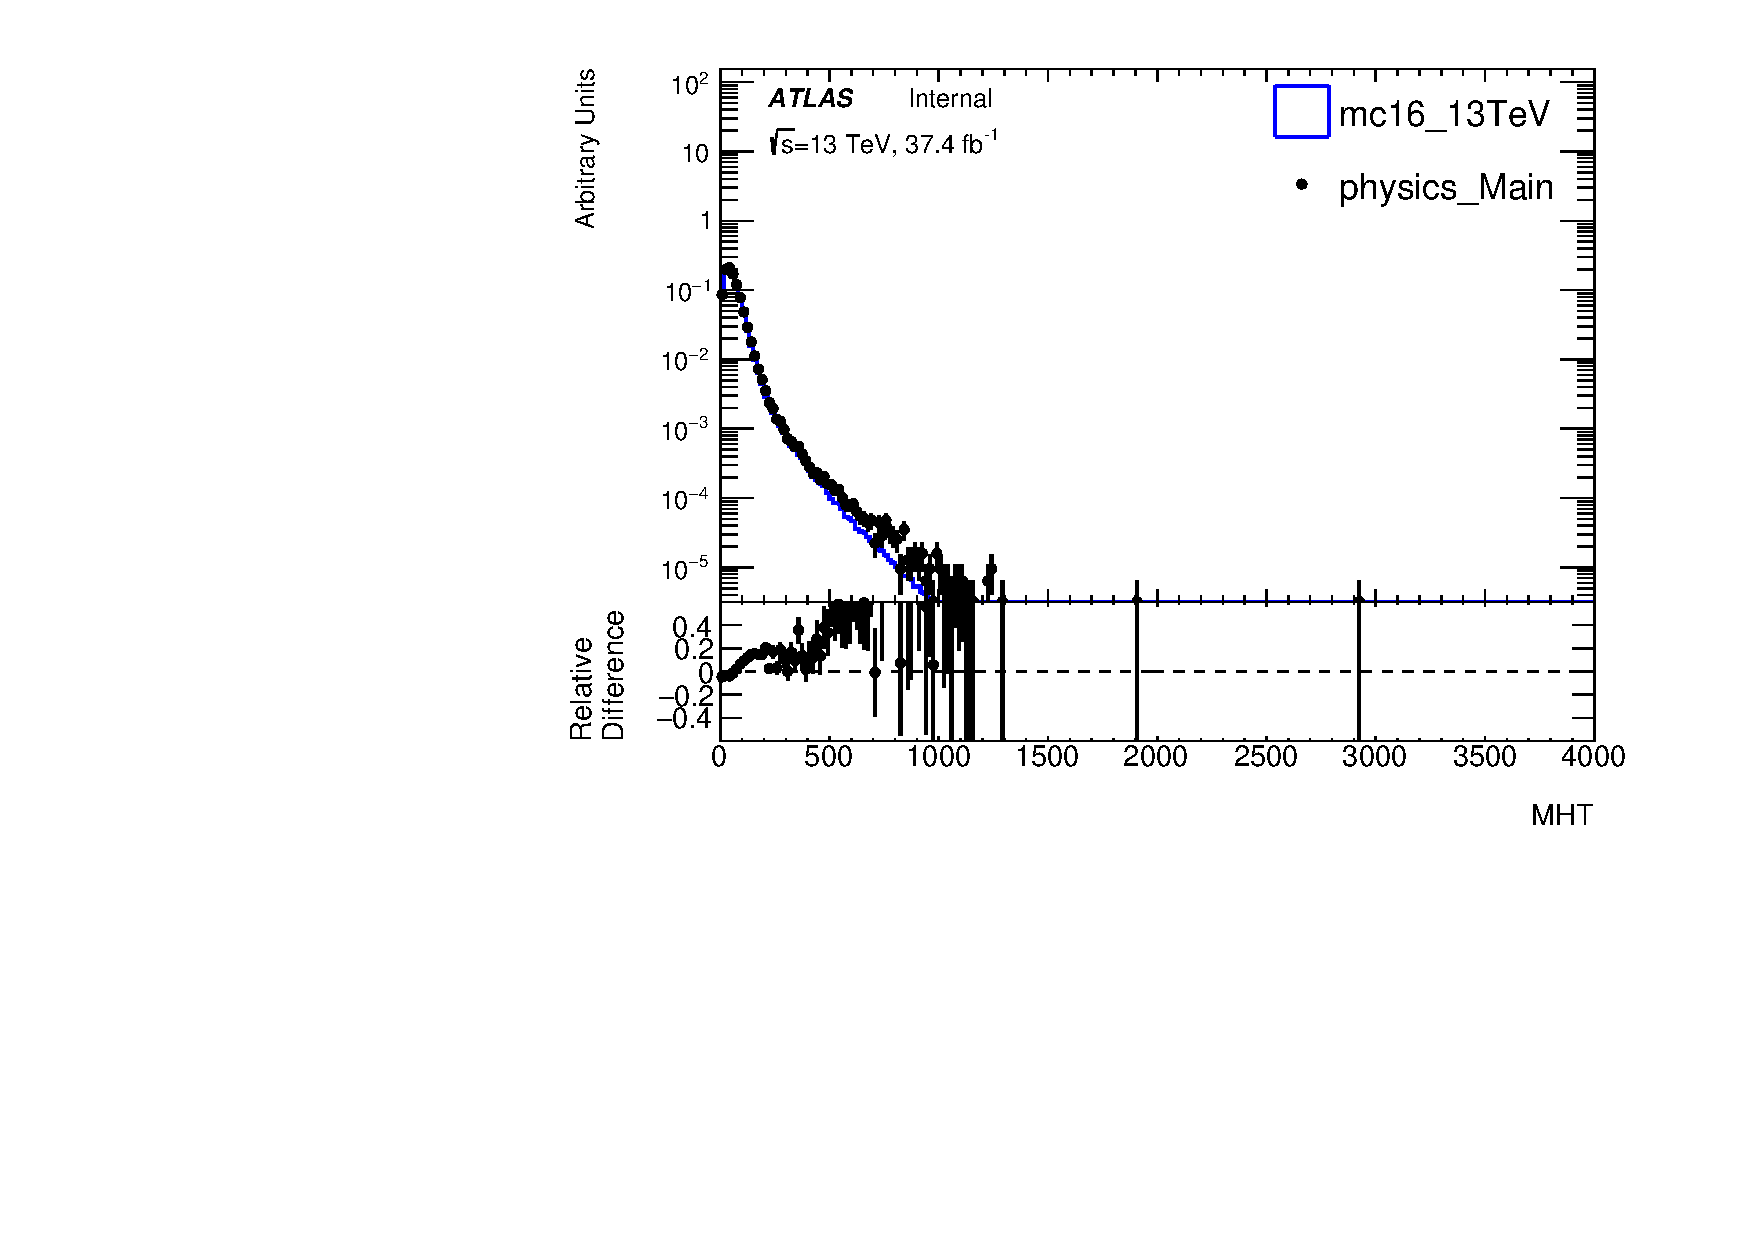
\includegraphics[width=0.45\textwidth]{figures/monitoring/resonant/2015-16/QQ/newStudy_MHT_logY_QQv01.pdf}}
% %
% \subfigure[] {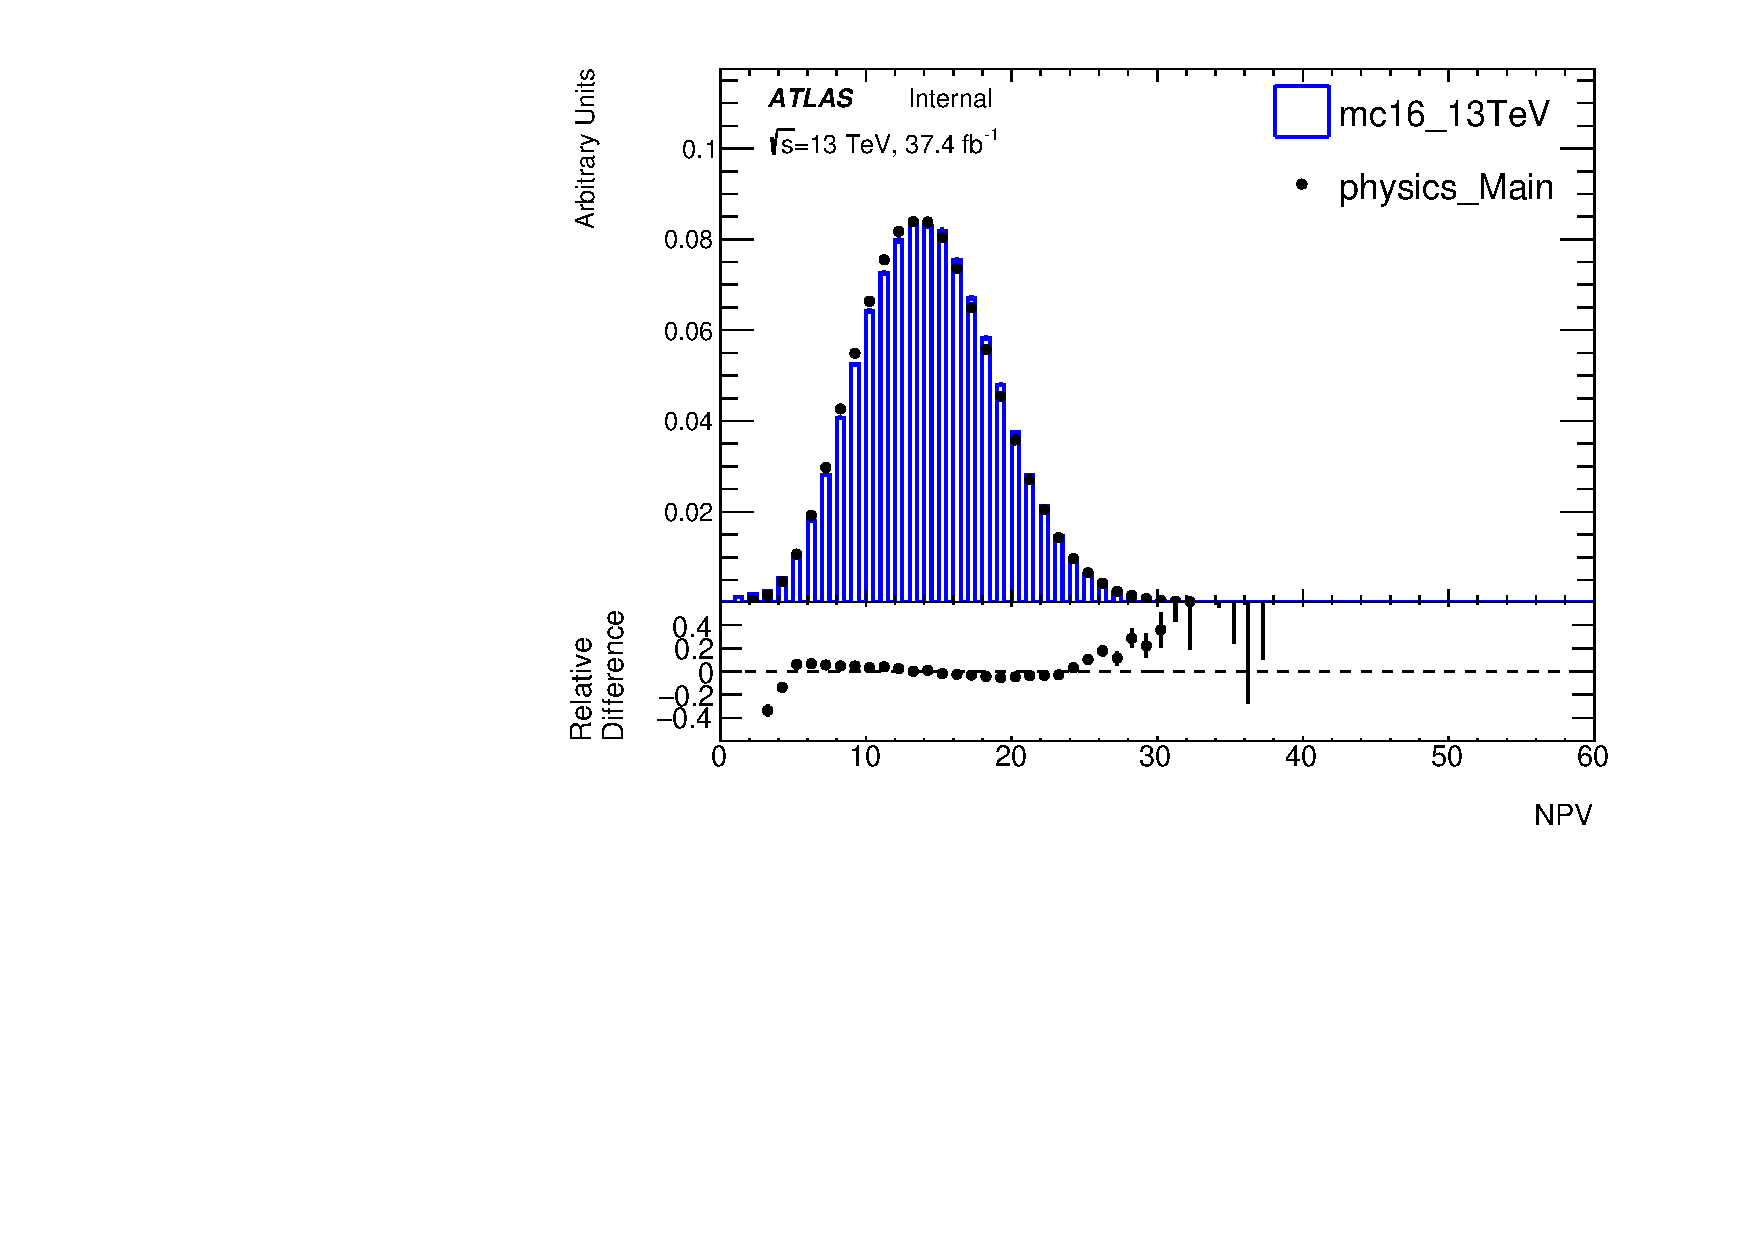
\includegraphics[width=0.45\textwidth]{figures/monitoring/resonant/2015-16/QQ/newStudy_NPV_QQv01.pdf}}
% \subfigure[] {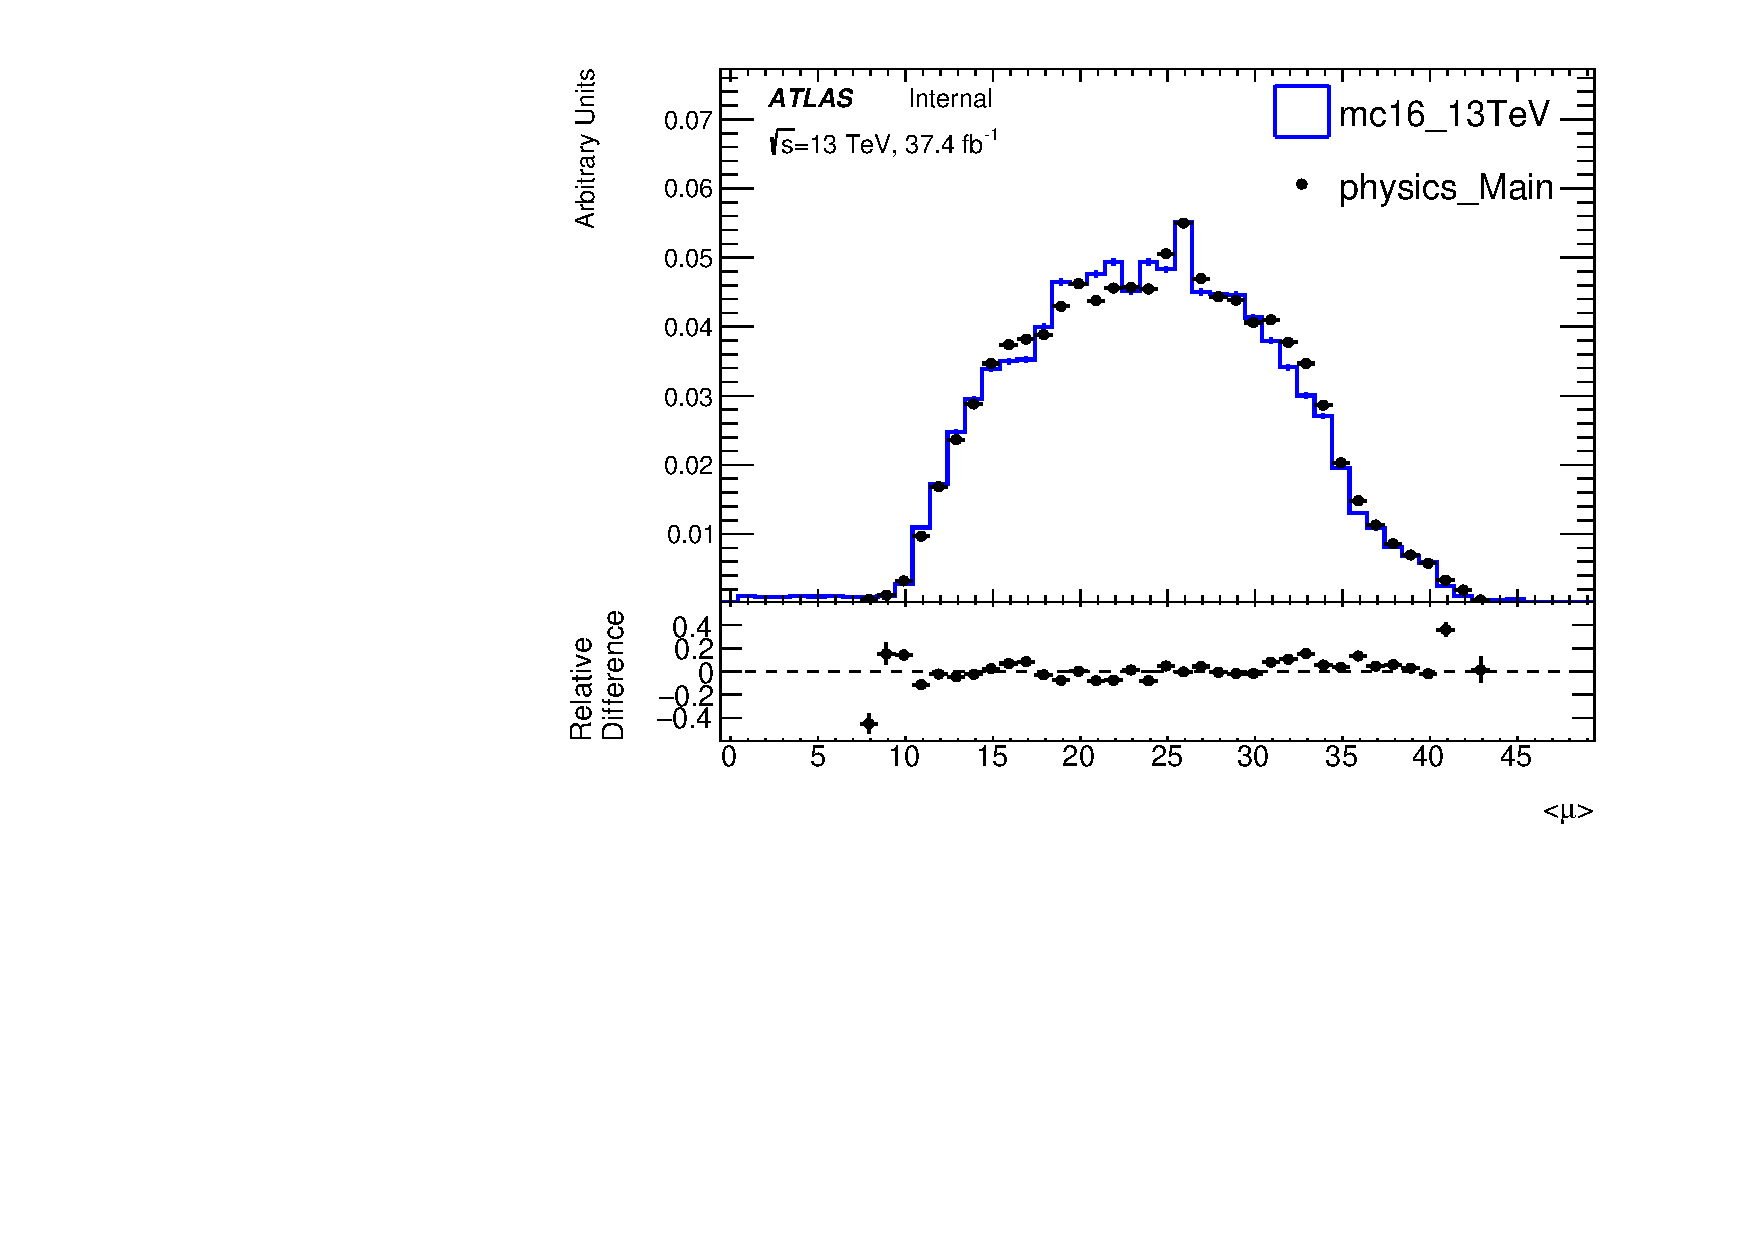
\includegraphics[width=0.45\textwidth]{figures/monitoring/resonant/2015-16/QQ/newStudy_averageInteractionsPerCrossing_QQv01.pdf}}
% %
%
% \caption{Monitoring plots on %2016 data, 
% the QQ resonant selection. (a) $H_T$, (b) $MH_T$ (missing transverse momentum calculated only from the jets in the event), (c) number of primary interaction vertices and (d) average interactions per bunch crossing.}
% \label{fig:QQmonitoring1}
%\end{figure}
%
% \begin{figure}[htb]
% \centering
%  %
% \subfigure[] {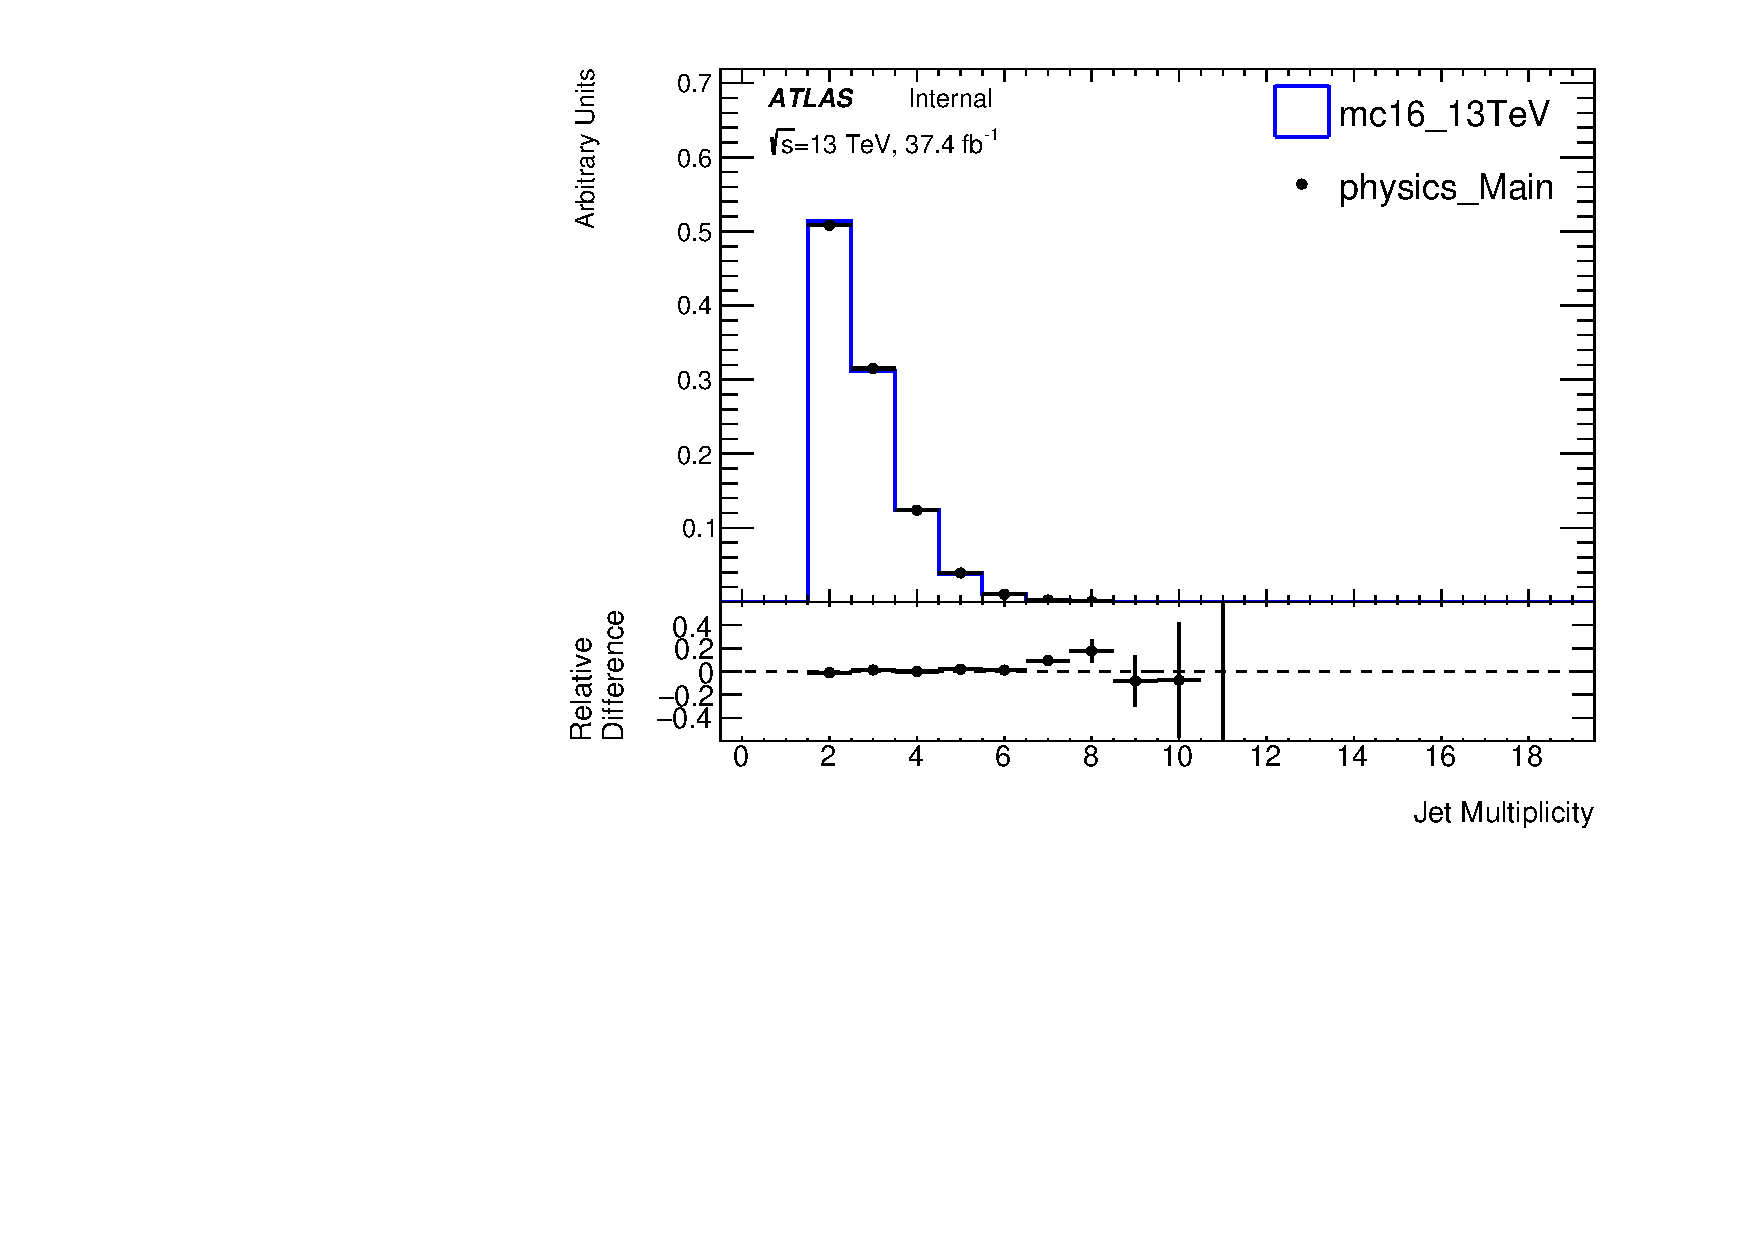
\includegraphics[width=0.45\textwidth]{figures/monitoring/resonant/2015-16/QQ/newStudy_njets_QQv01.pdf}}
% \subfigure[] {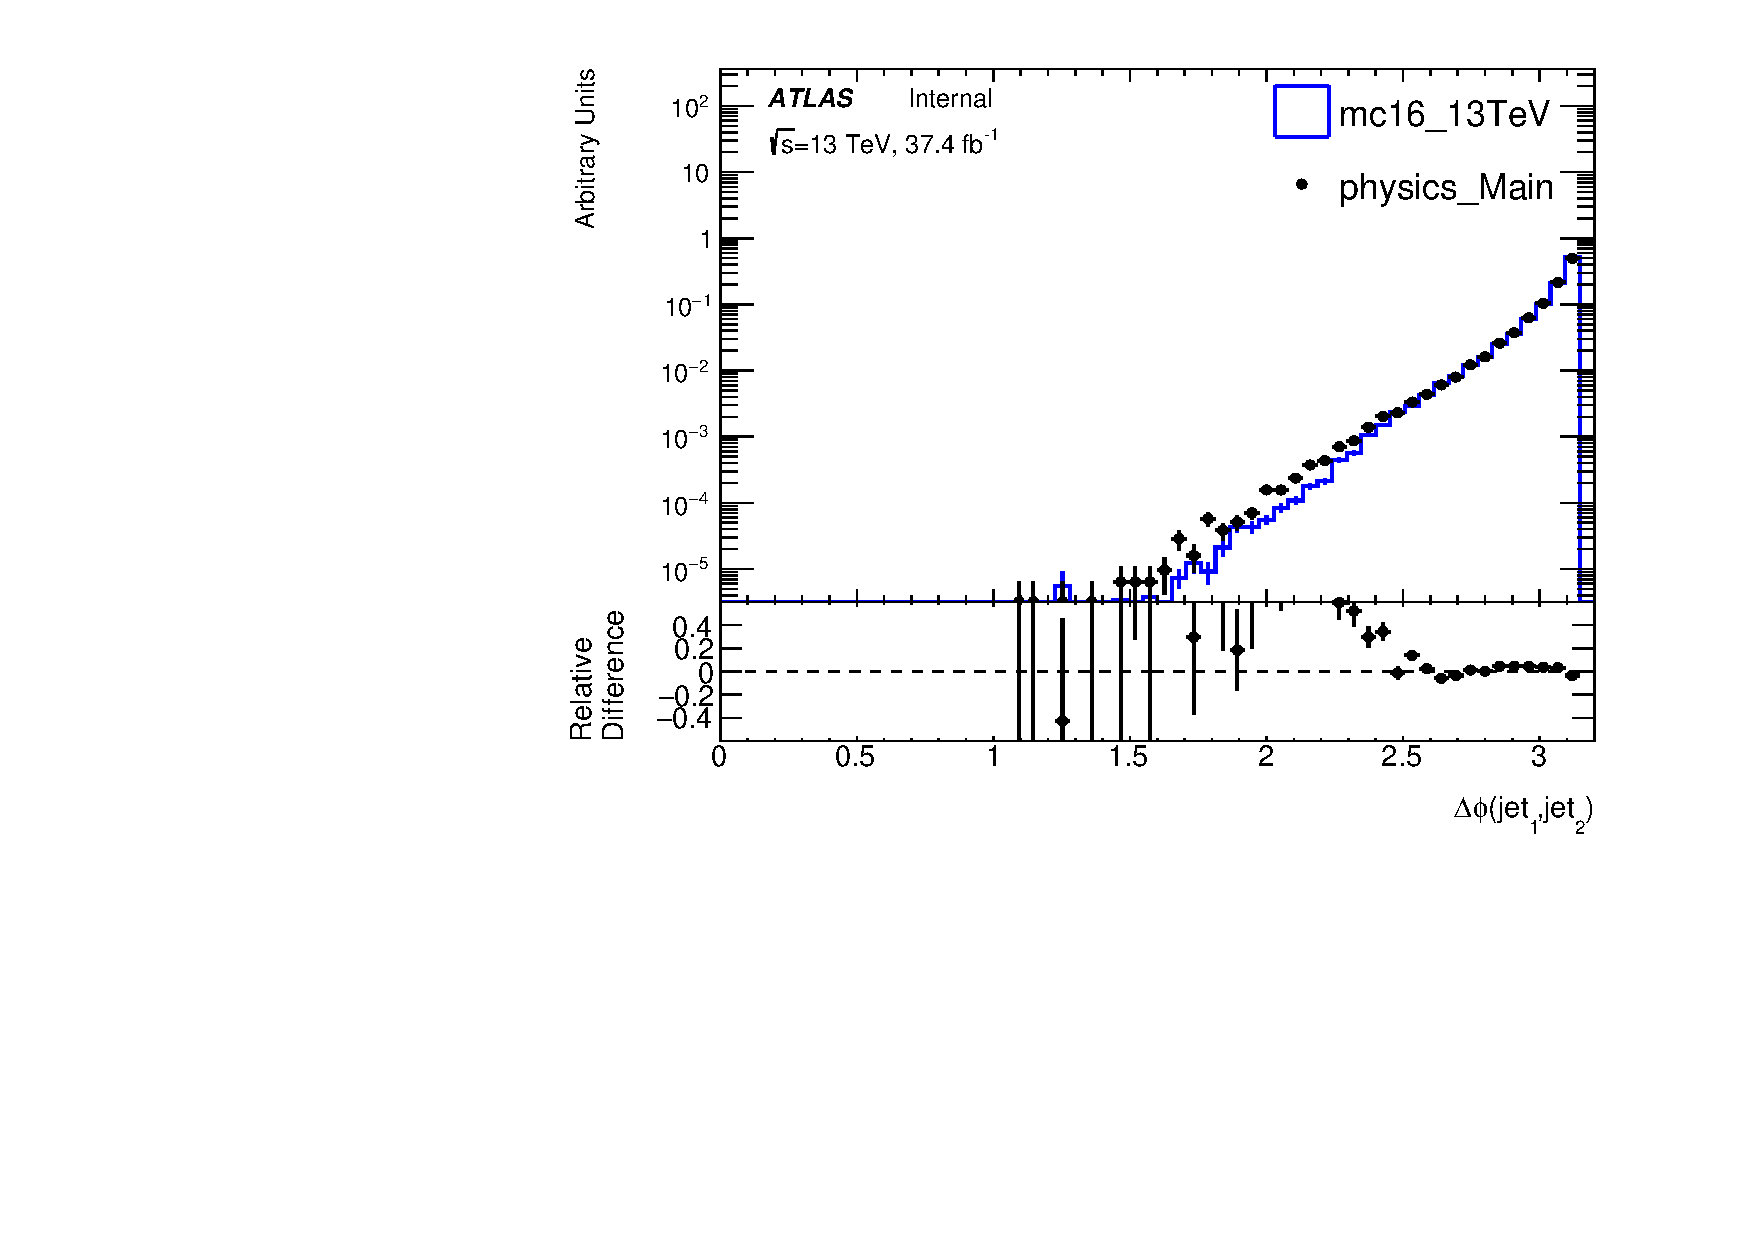
\includegraphics[width=0.45\textwidth]{figures/monitoring/resonant/2015-16/QQ//newStudy_deltaPhi_logY_QQv01.pdf}}
%
%%
% \subfigure[] {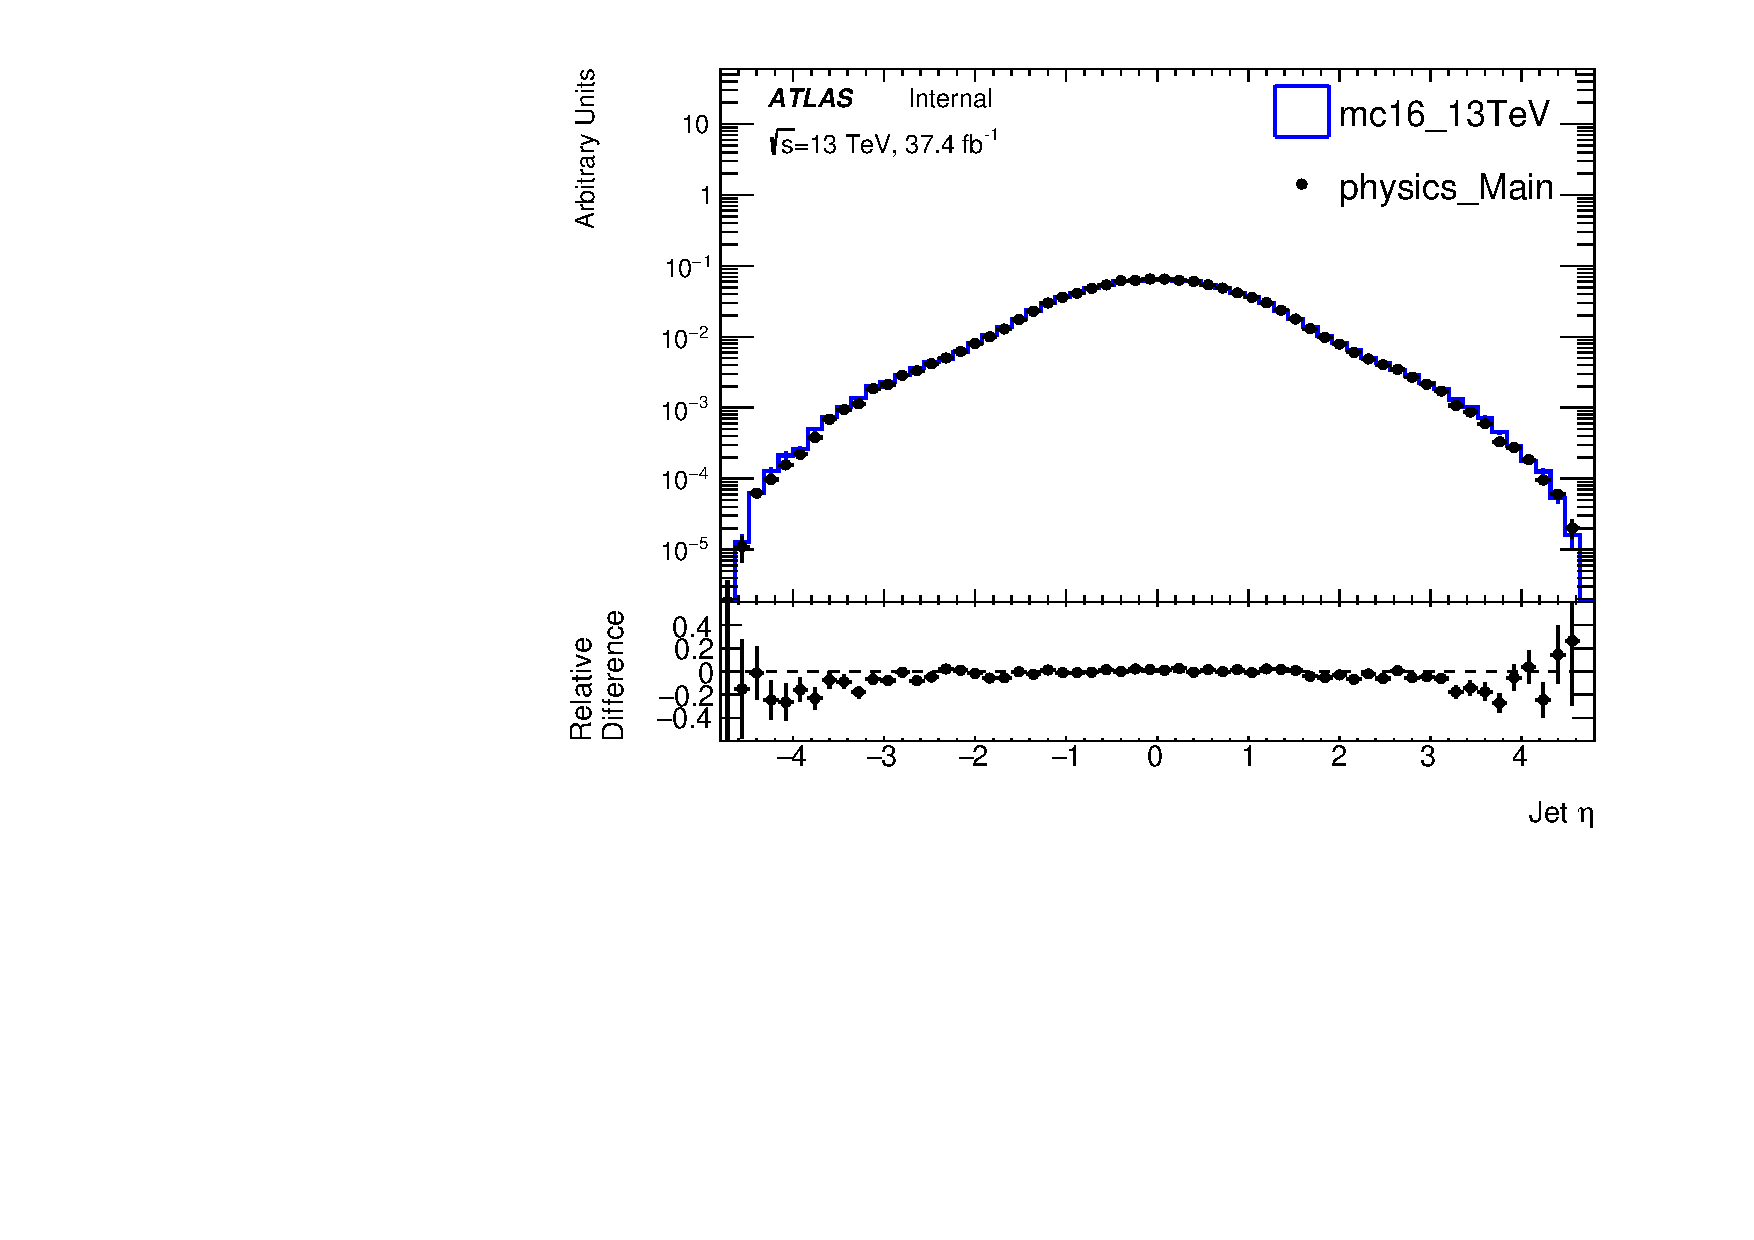
\includegraphics[width=0.45\textwidth]{figures/monitoring/resonant/2015-16/QQ/newStudy_jet_eta_logY_QQv01.pdf}}
% \subfigure[] {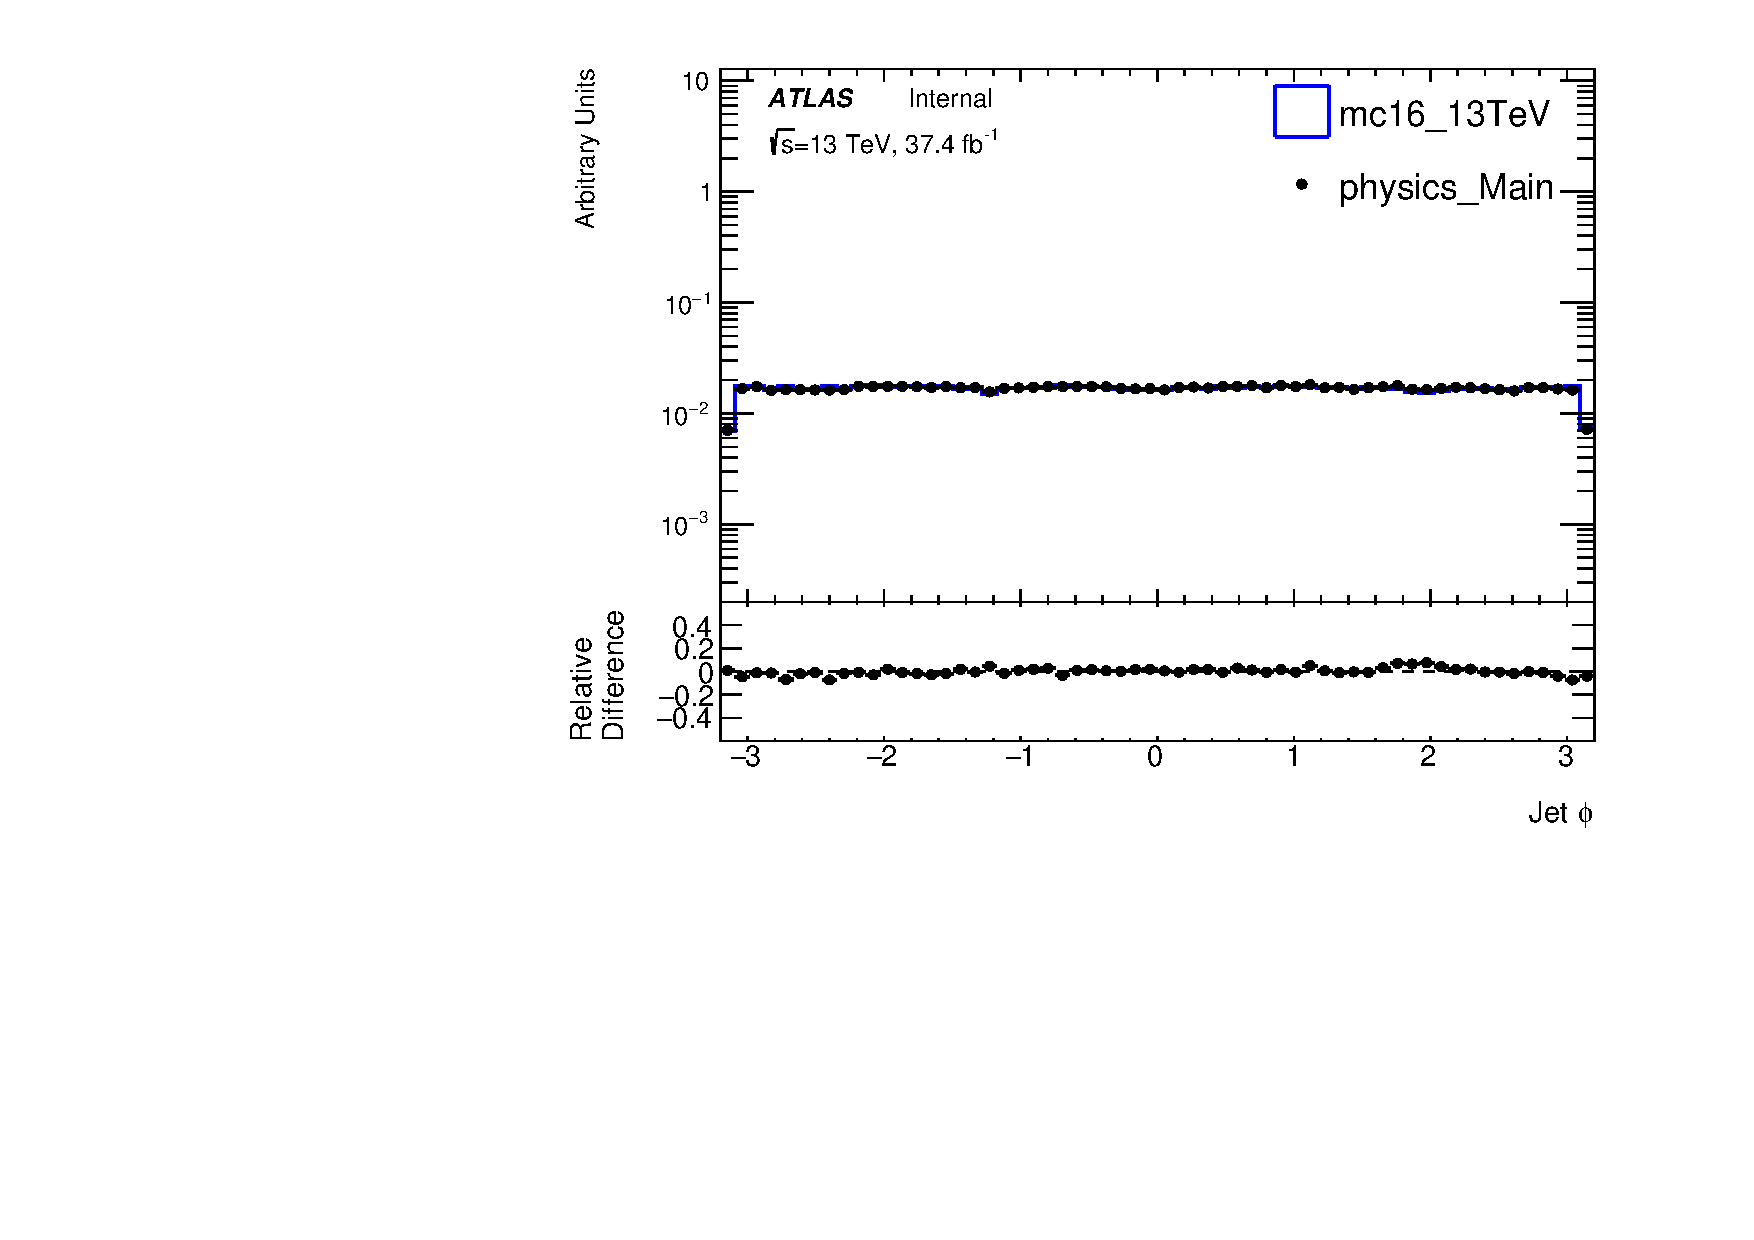
\includegraphics[width=0.45\textwidth]{figures/monitoring/resonant/2015-16/QQ/newStudy_jet_phi_logY_QQv01.pdf}}
% %
% \subfigure[] {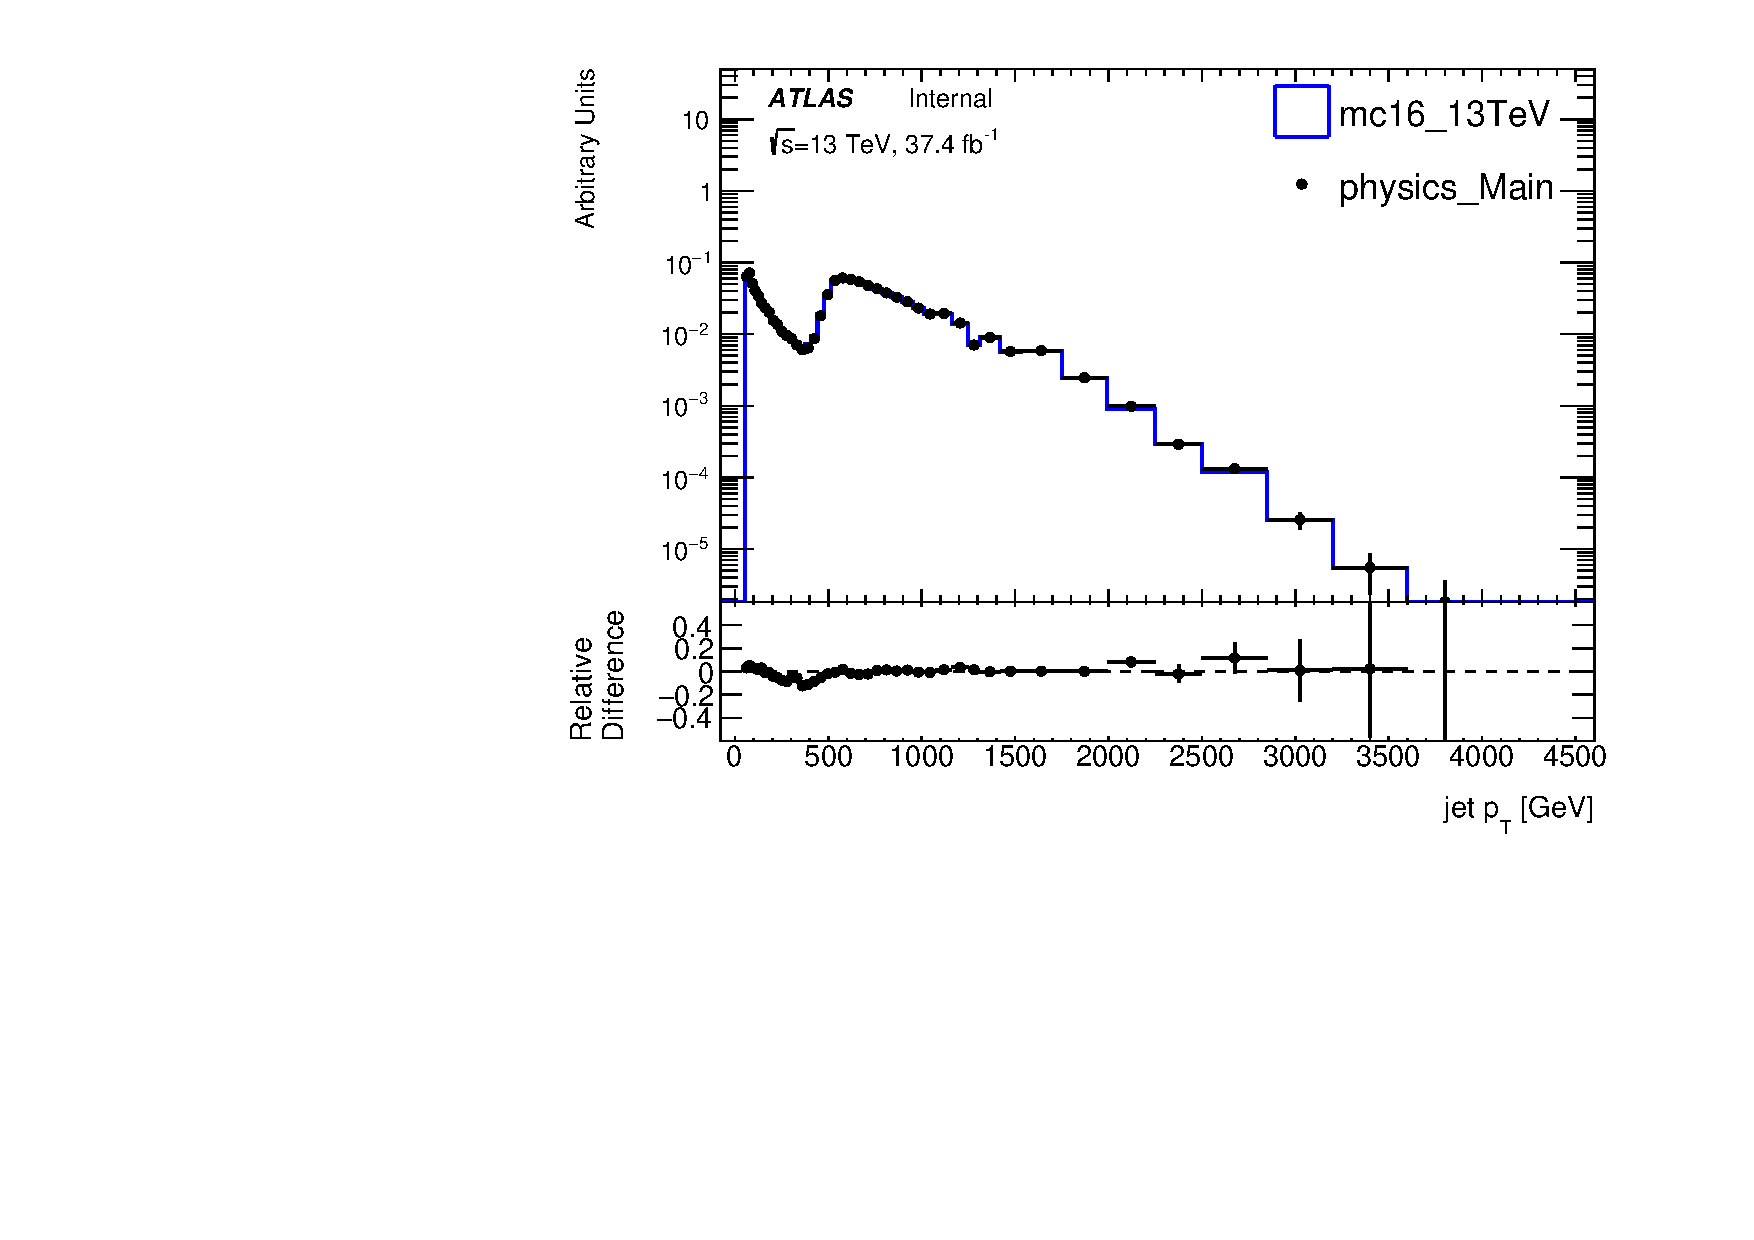
\includegraphics[width=0.45\textwidth]{figures/monitoring/resonant/2015-16/QQ/newStudy_jet_pt_logY_QQv01.pdf}}
% \subfigure[] {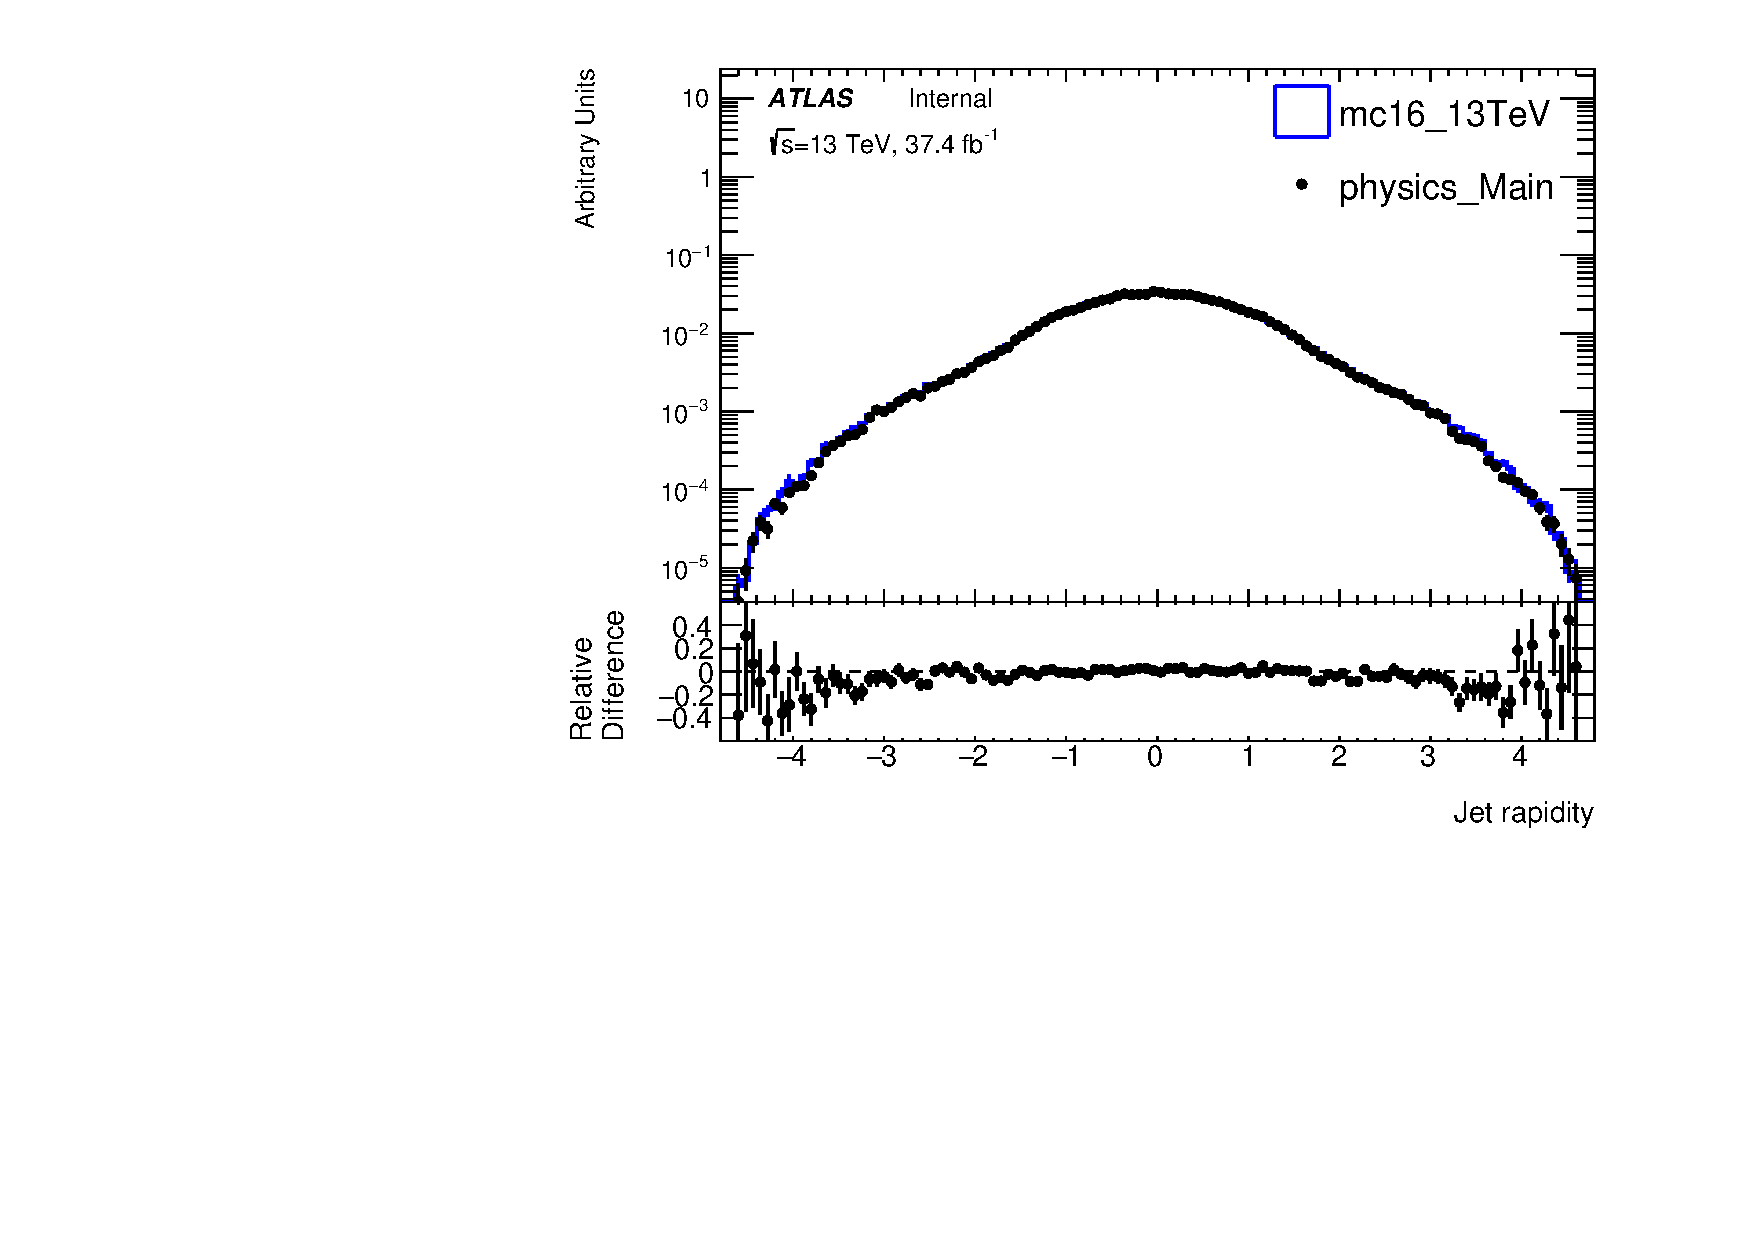
\includegraphics[width=0.45\textwidth]{figures/monitoring/resonant/2015-16/QQ/newStudy_jet_rapidity_logY_QQv01.pdf}}
% %
% 
%  \caption{Jet plots on %2016 data, 
%  the resonant selection. (a) number of jets (b) $\Delta\phi$ between the two jets (c) jet $\eta$
%  (d) jet $\phi$ (e) jet \pT\ (f) jet rapidity.  Fluctuations in the jet $phi$ distribution are attributable to dead modules in the tile calorimeter which lead to fewer jets in small slices of the detector.}
% \label{fig:QQmonitoring5}
%\end{figure}
%
%
% \begin{figure}[htb]
% \centering
% %
% \subfigure[] {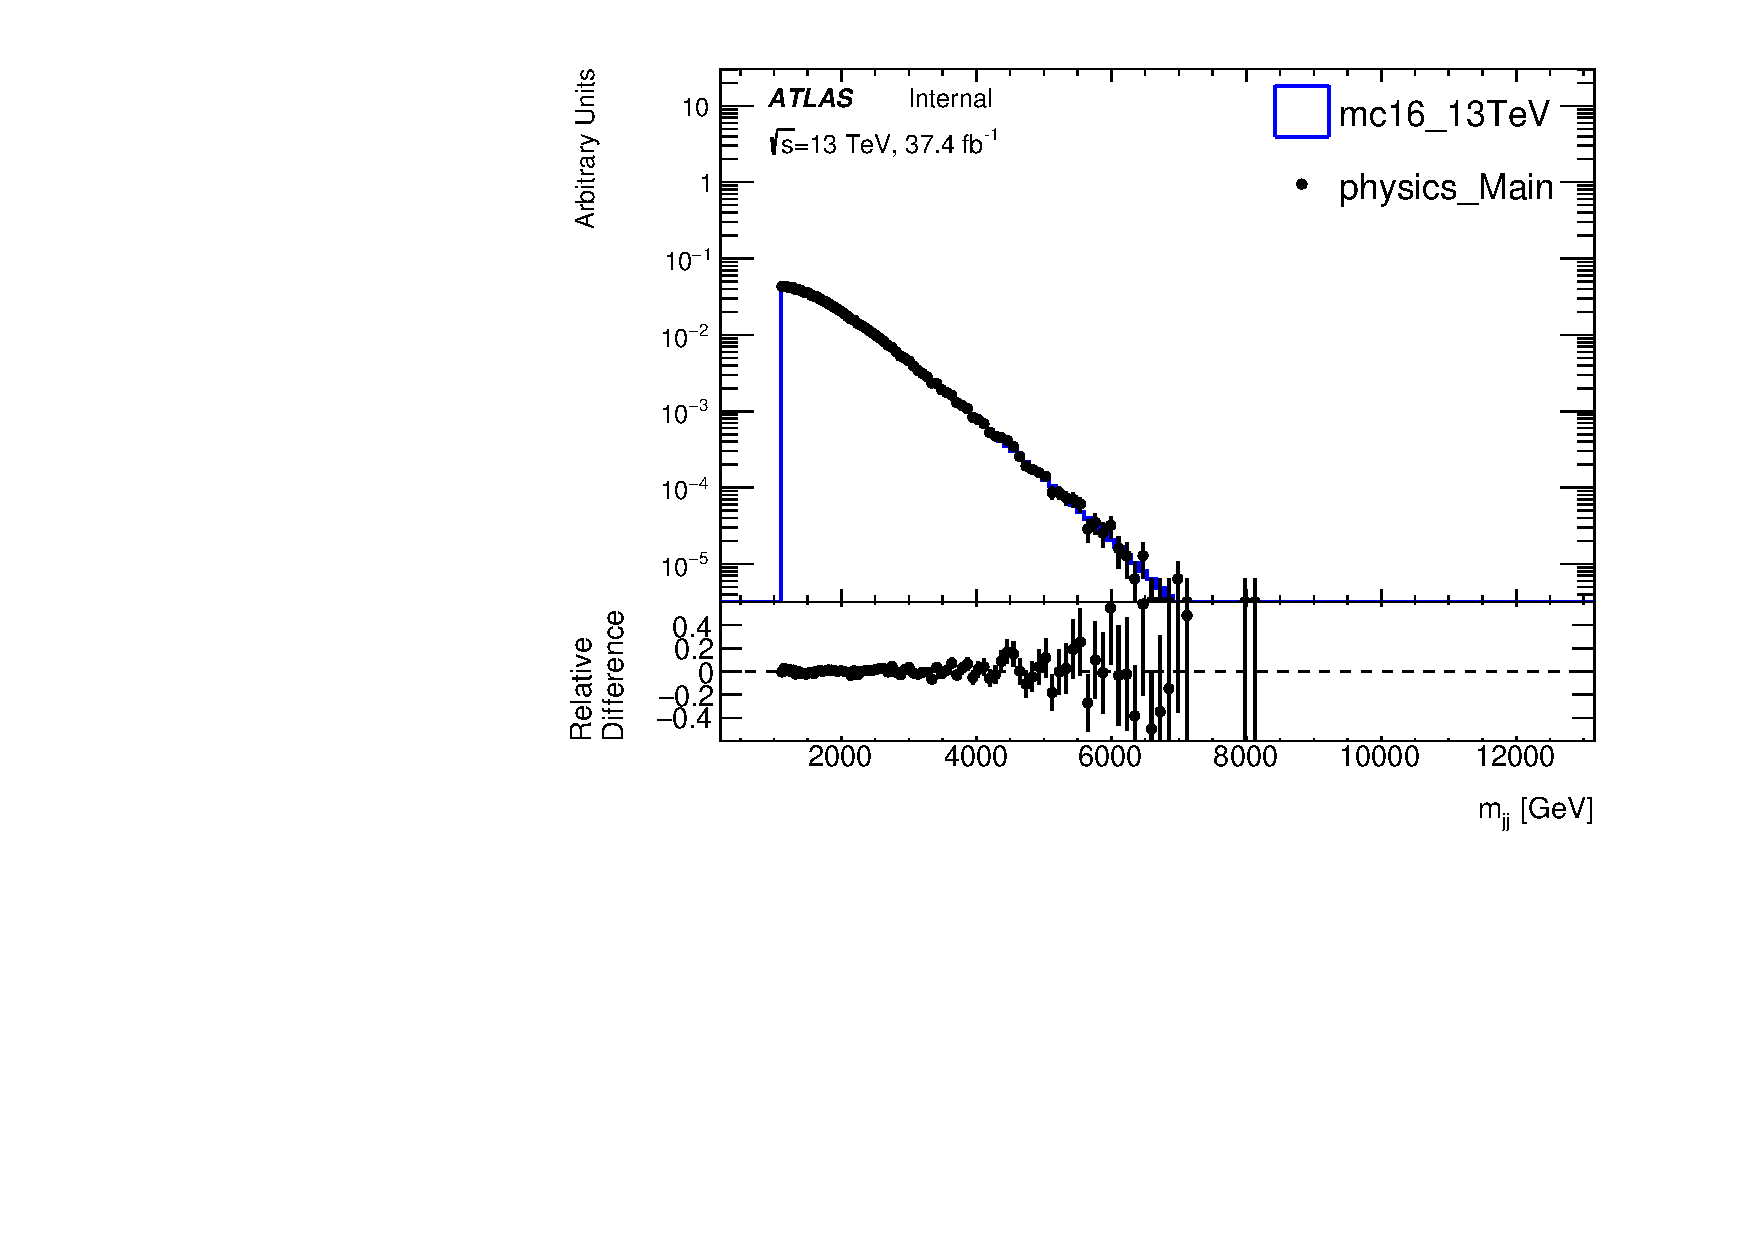
\includegraphics[width=0.45\textwidth]{figures/monitoring/resonant/2015-16/QQ/newStudy_mjj_logY_QQv01.pdf}}
% \subfigure[] {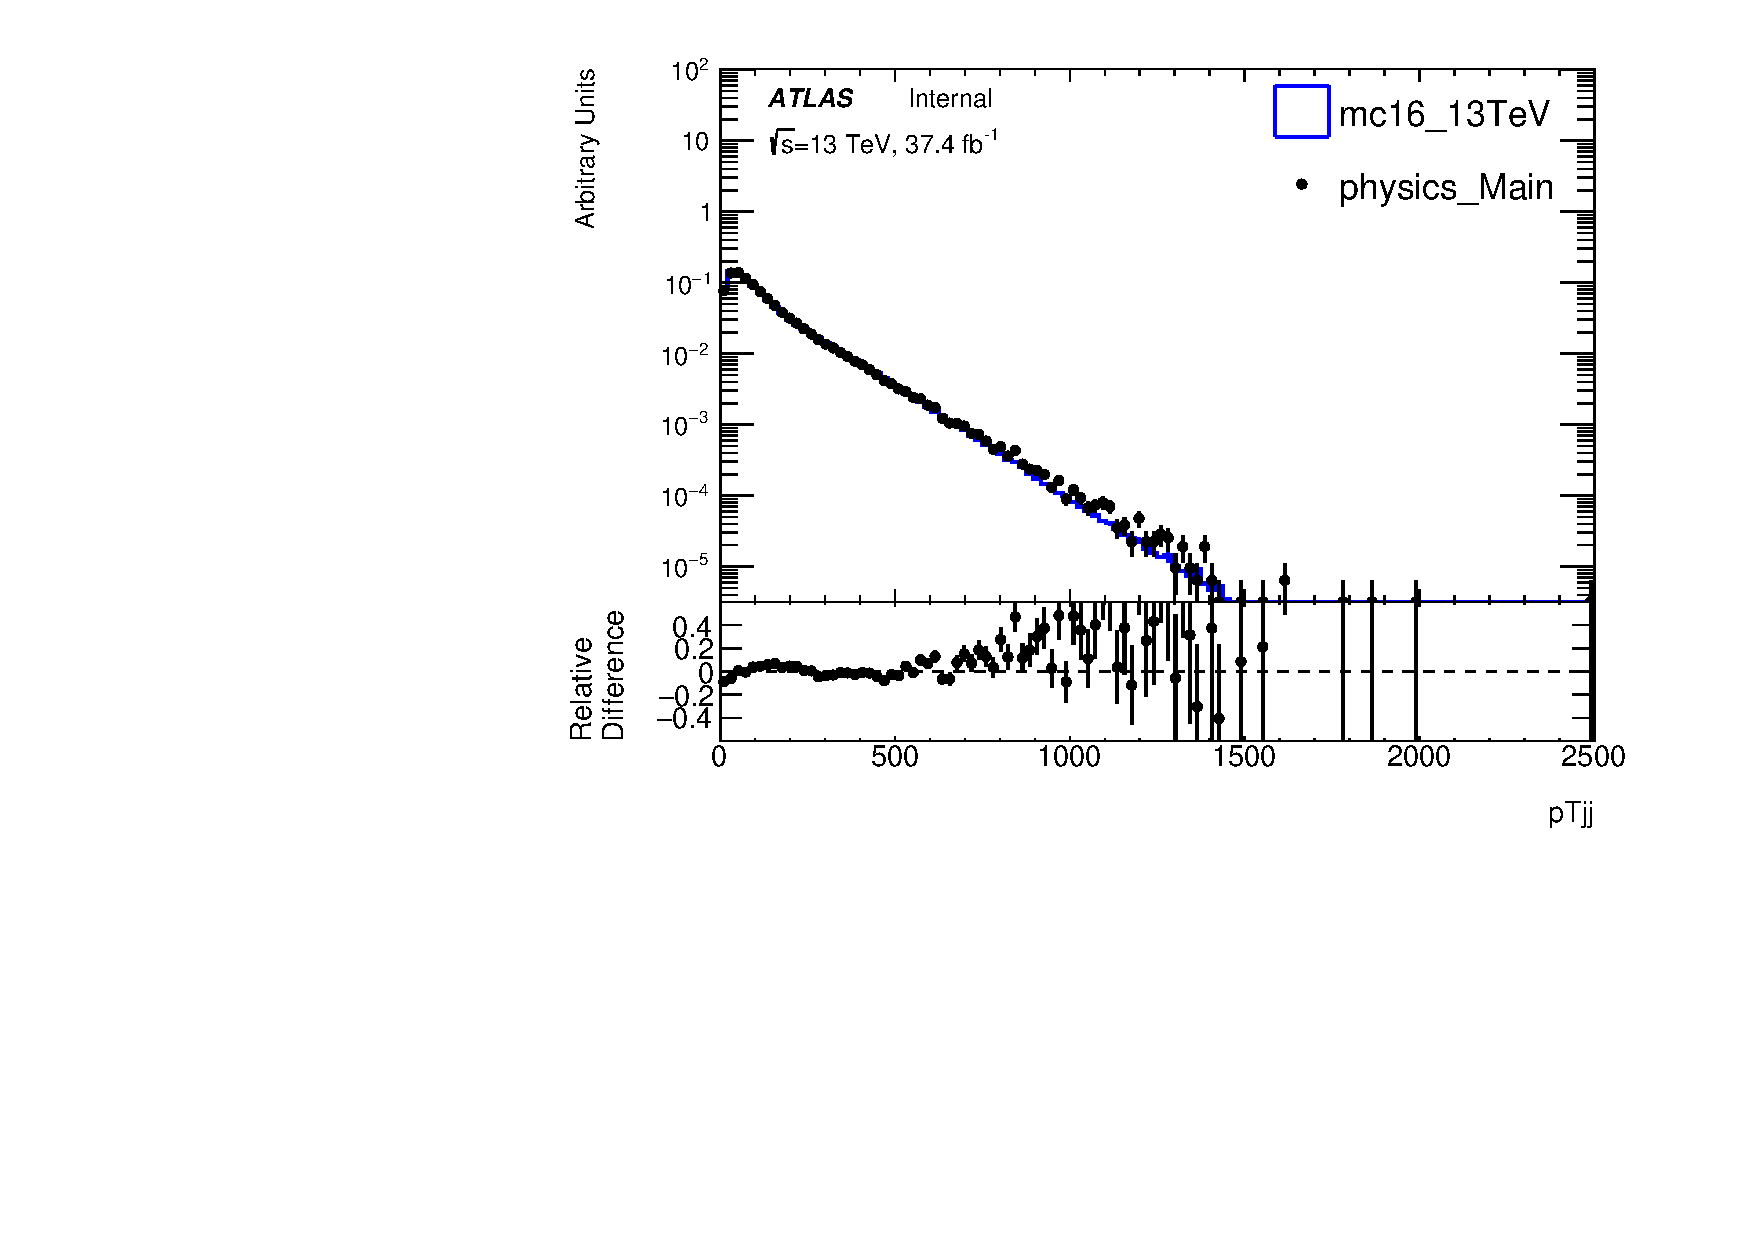
\includegraphics[width=0.45\textwidth]{figures/monitoring/resonant/2015-16/QQ/newStudy_pTjj_logY_QQv01.pdf}}
% %
% \subfigure[] {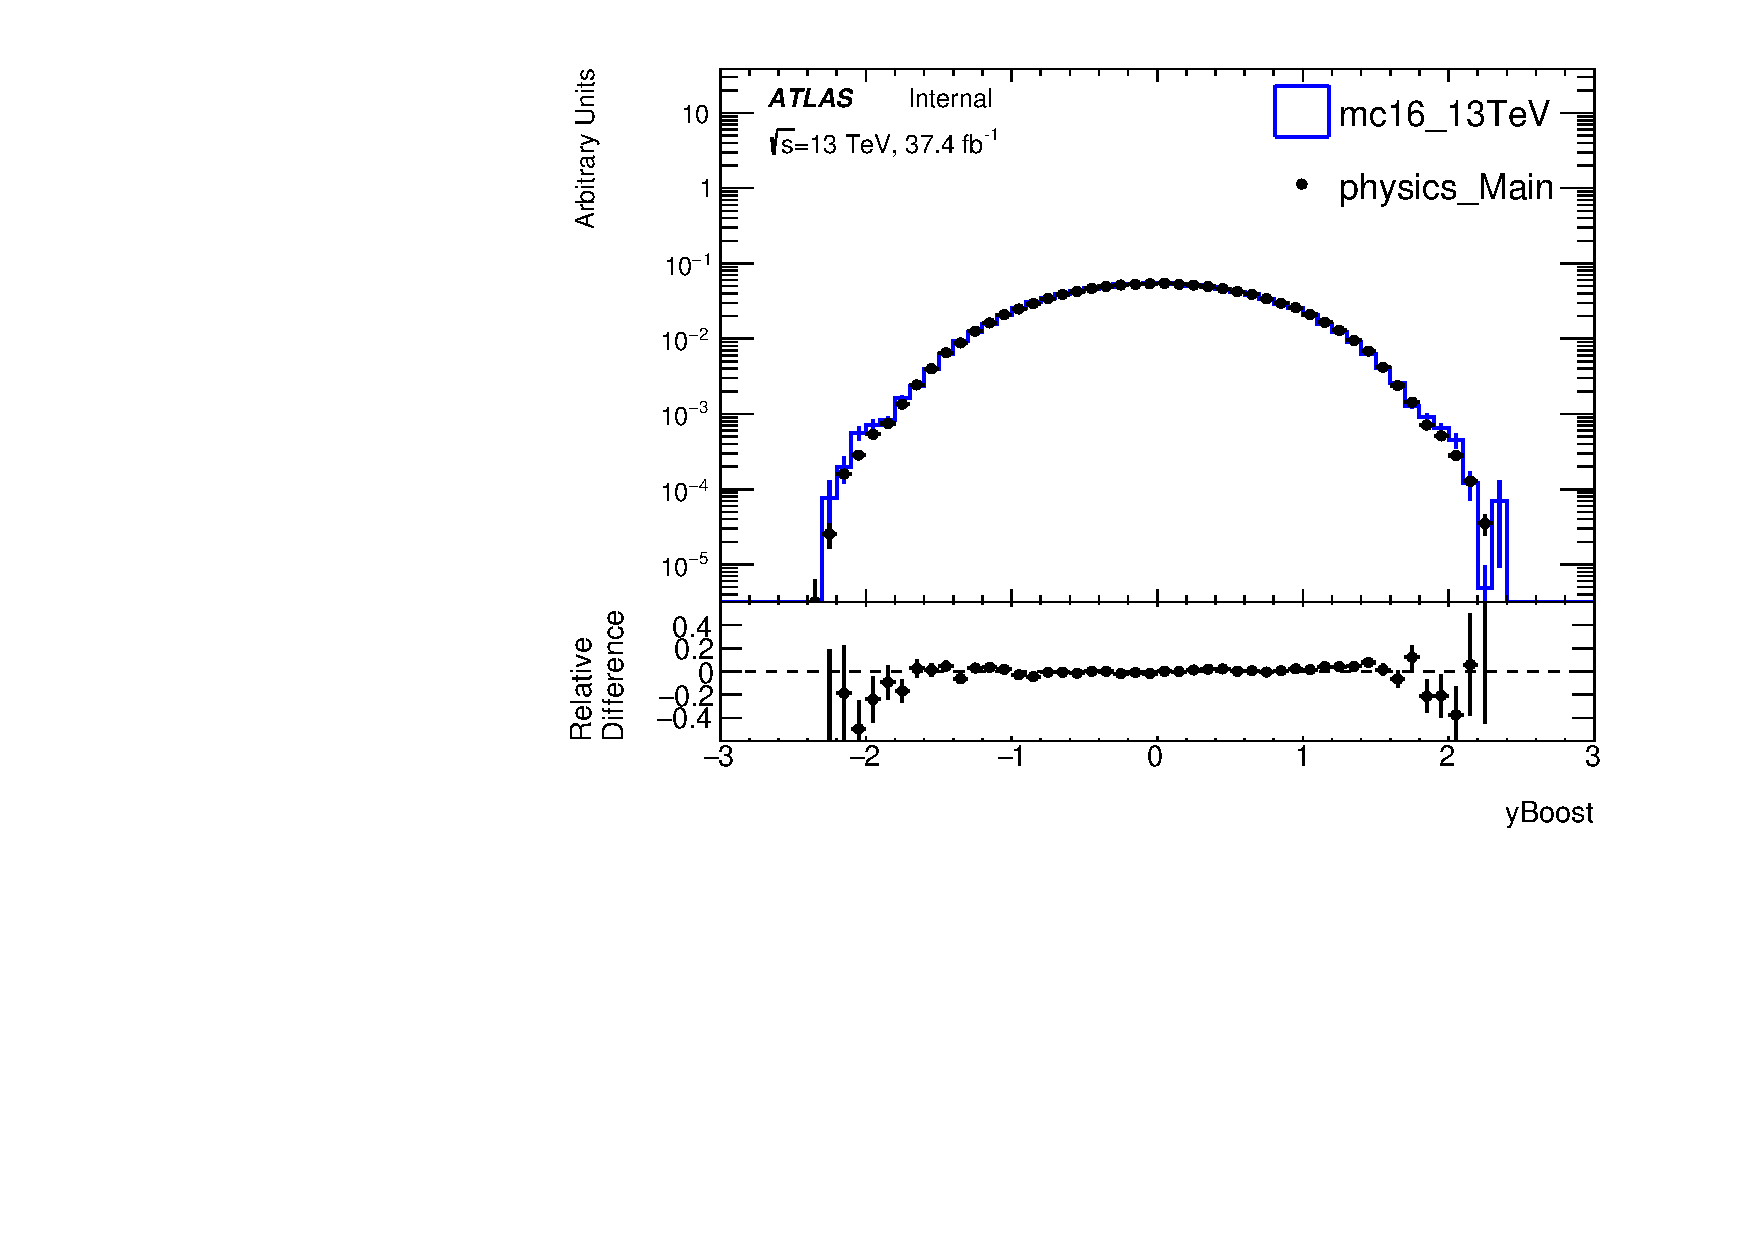
\includegraphics[width=0.45\textwidth]{figures/monitoring/resonant/2015-16/QQ/newStudy_yBoost_logY_QQv01.pdf}}
% \subfigure[] {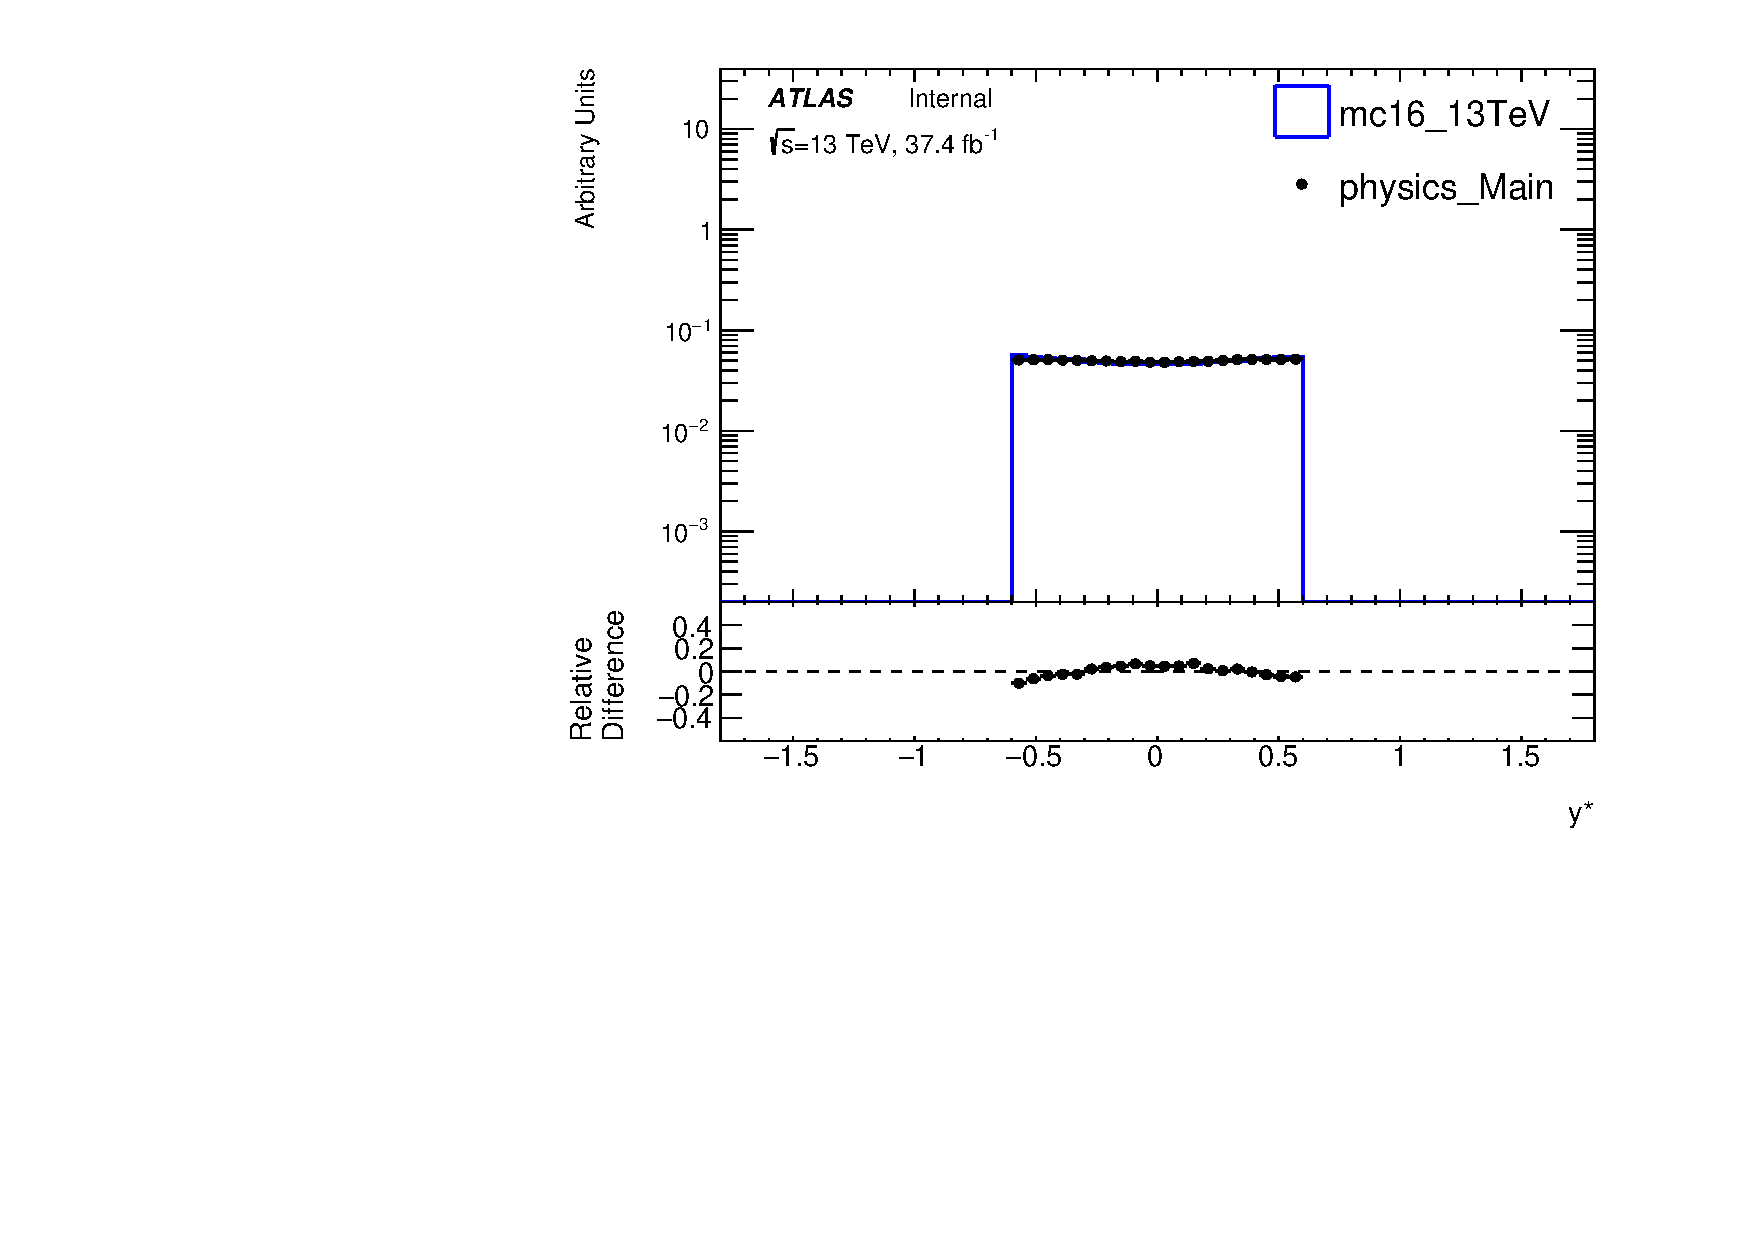
\includegraphics[width=0.45\textwidth]{figures/monitoring/resonant/2015-16/QQ/newStudy_yStar_logY_QQv01.pdf}}
% \caption{Jet plots on %2016 data, 
% the resonant selection. (a) dijet invariant mass (b) dijet \pT\ (c) \yB{} (d) \ystar{}. }
% \label{fig:QQmonitoring6}
%\end{figure}
%
%\clearpage
%
%In this section a selection of kinematic and monitoring plots produced with the resonant selection on the QG dataset is shown 
%(Figures~\ref{fig:QGmonitoring1},  
%\ref{fig:QGmonitoring5}, \ref{fig:QGmonitoring6}). These plots are relative to \integLumi of data collected in 2015 and 2016.
% GRL has been applied here.
%
%\begin{figure}[htb]
% \centering
% \subfigure[] {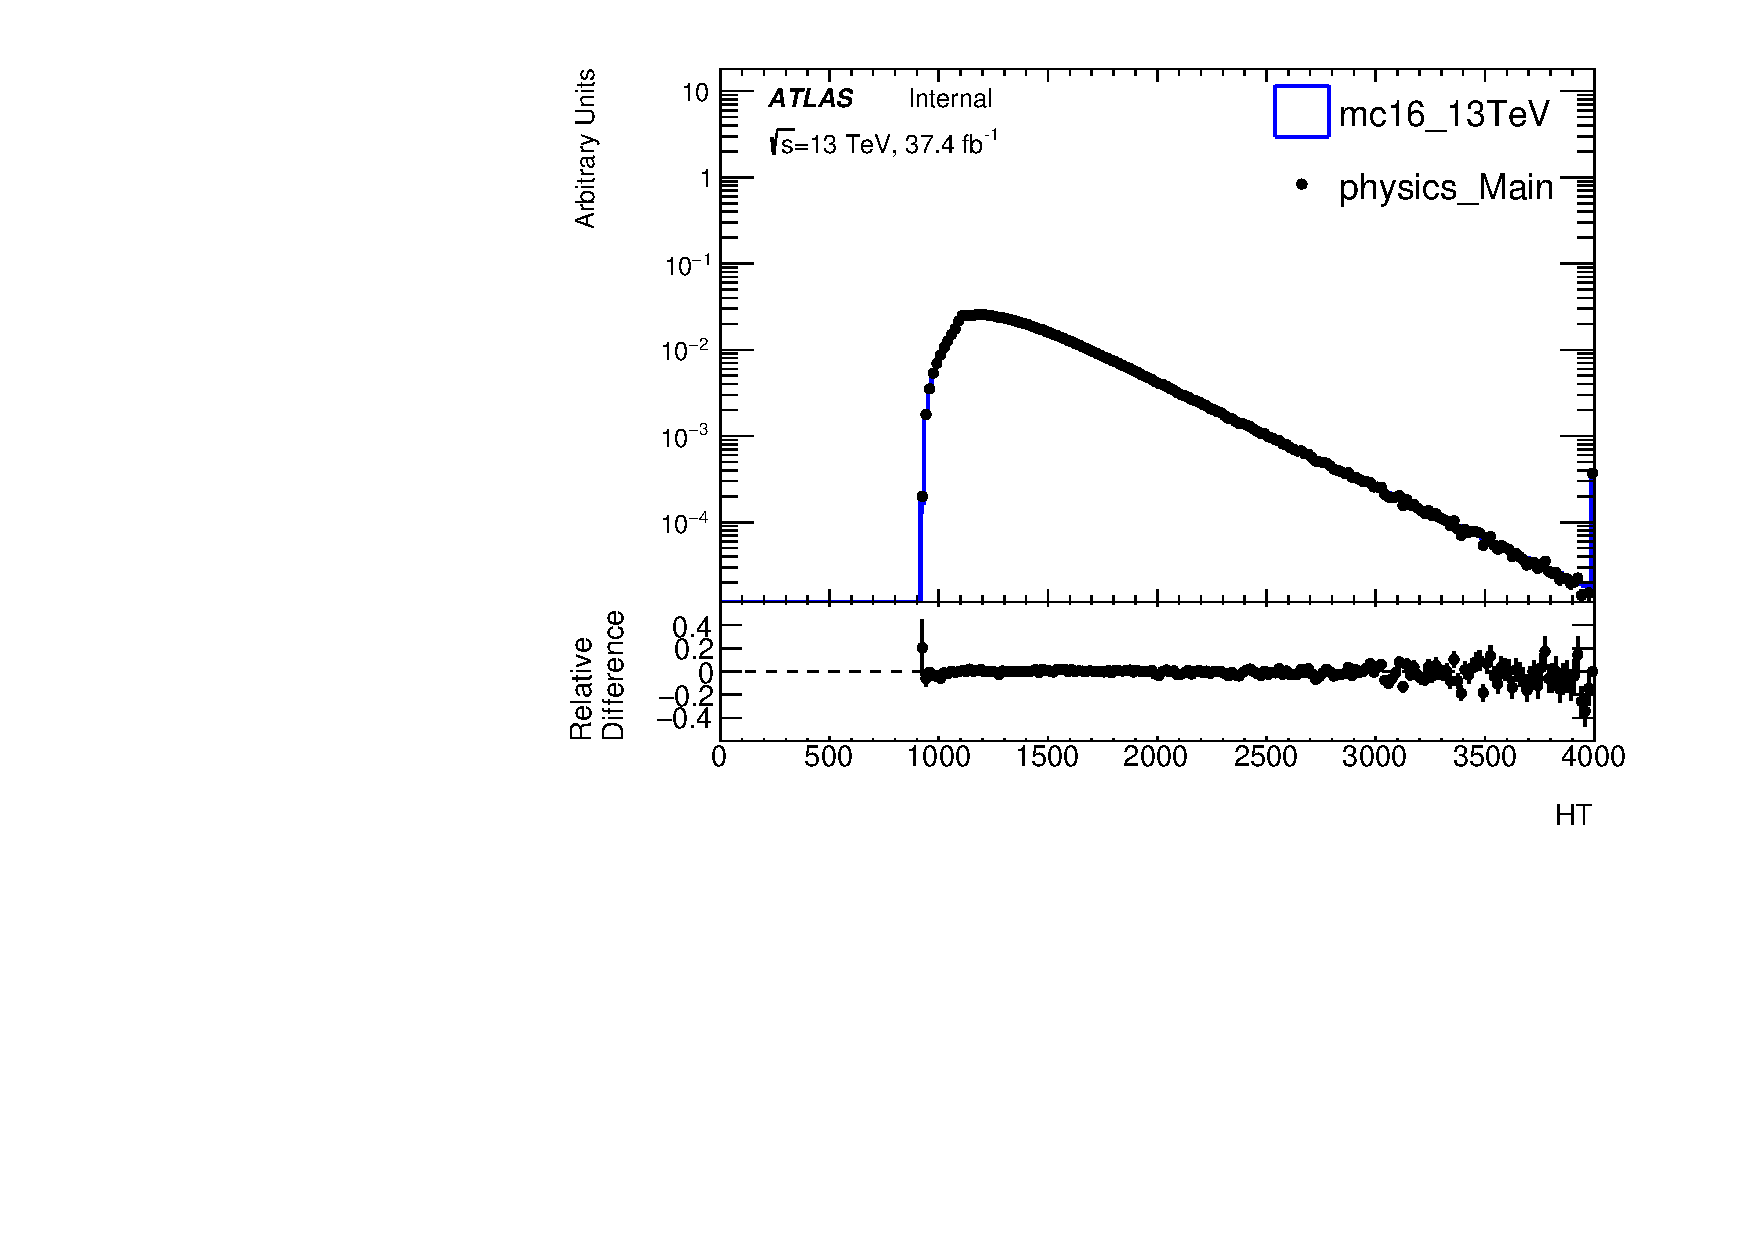
\includegraphics[width=0.45\textwidth]{figures/monitoring/resonant/2015-16/QG/newStudy_HT_logY_QGv01.pdf}}
% \subfigure[] {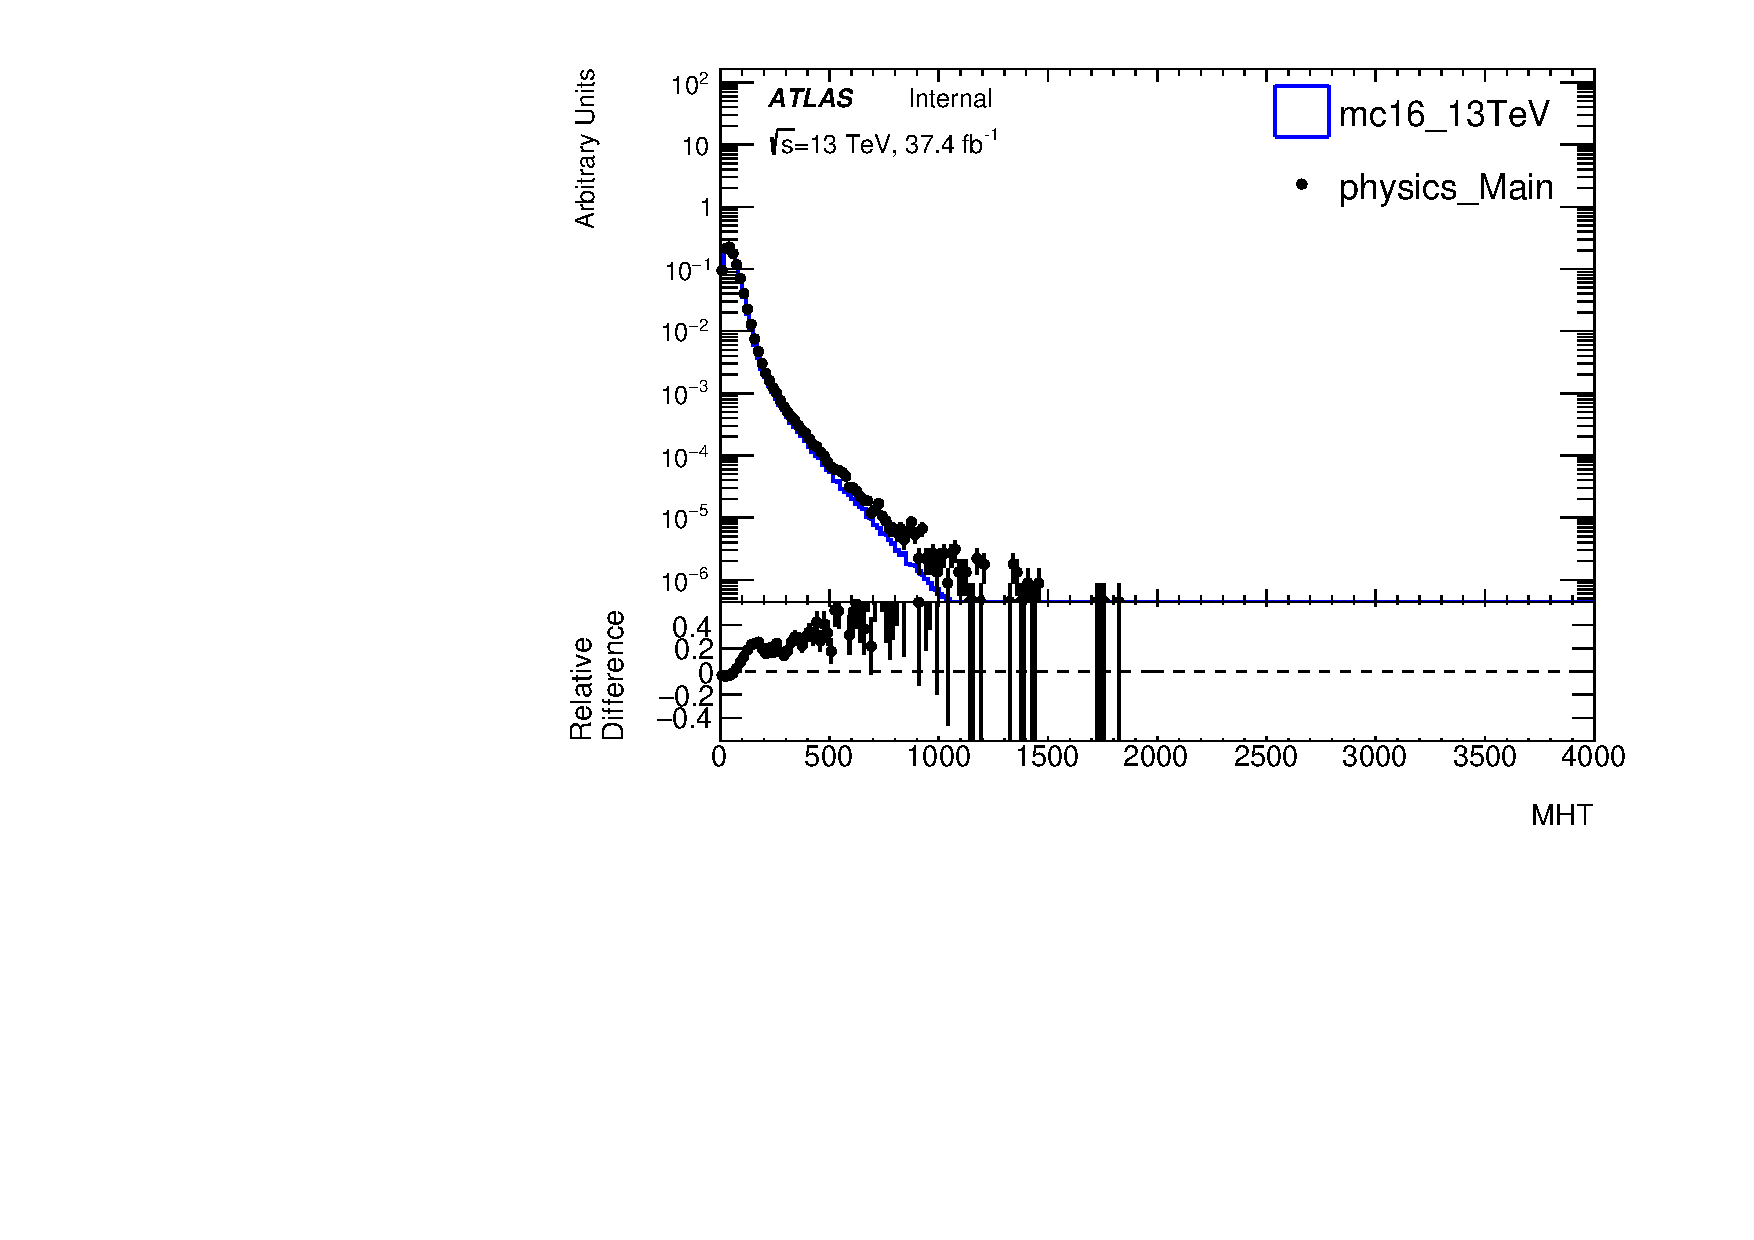
\includegraphics[width=0.45\textwidth]{figures/monitoring/resonant/2015-16/QG/newStudy_MHT_logY_QGv01.pdf}}
% %
% \subfigure[] {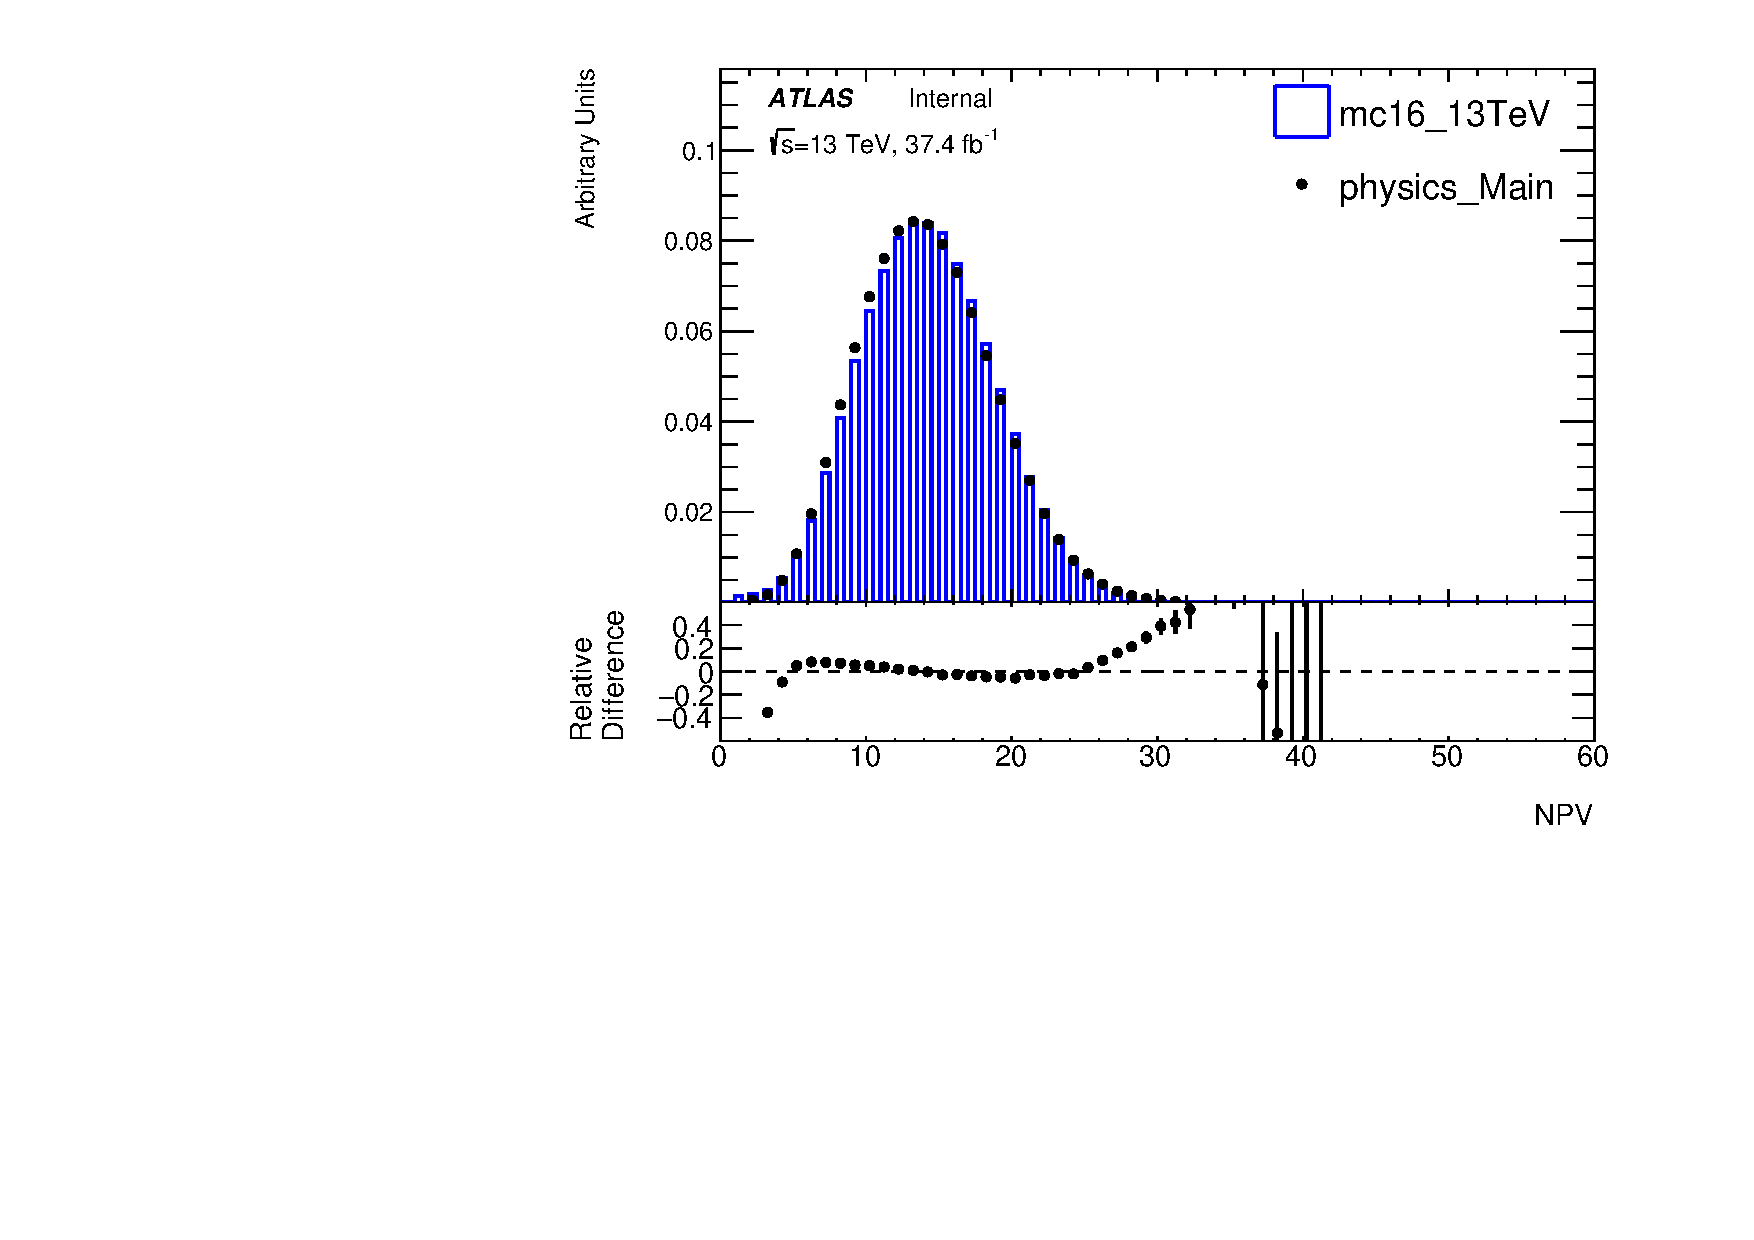
\includegraphics[width=0.45\textwidth]{figures/monitoring/resonant/2015-16/QG/newStudy_NPV_QGv01.pdf}}
% \subfigure[] {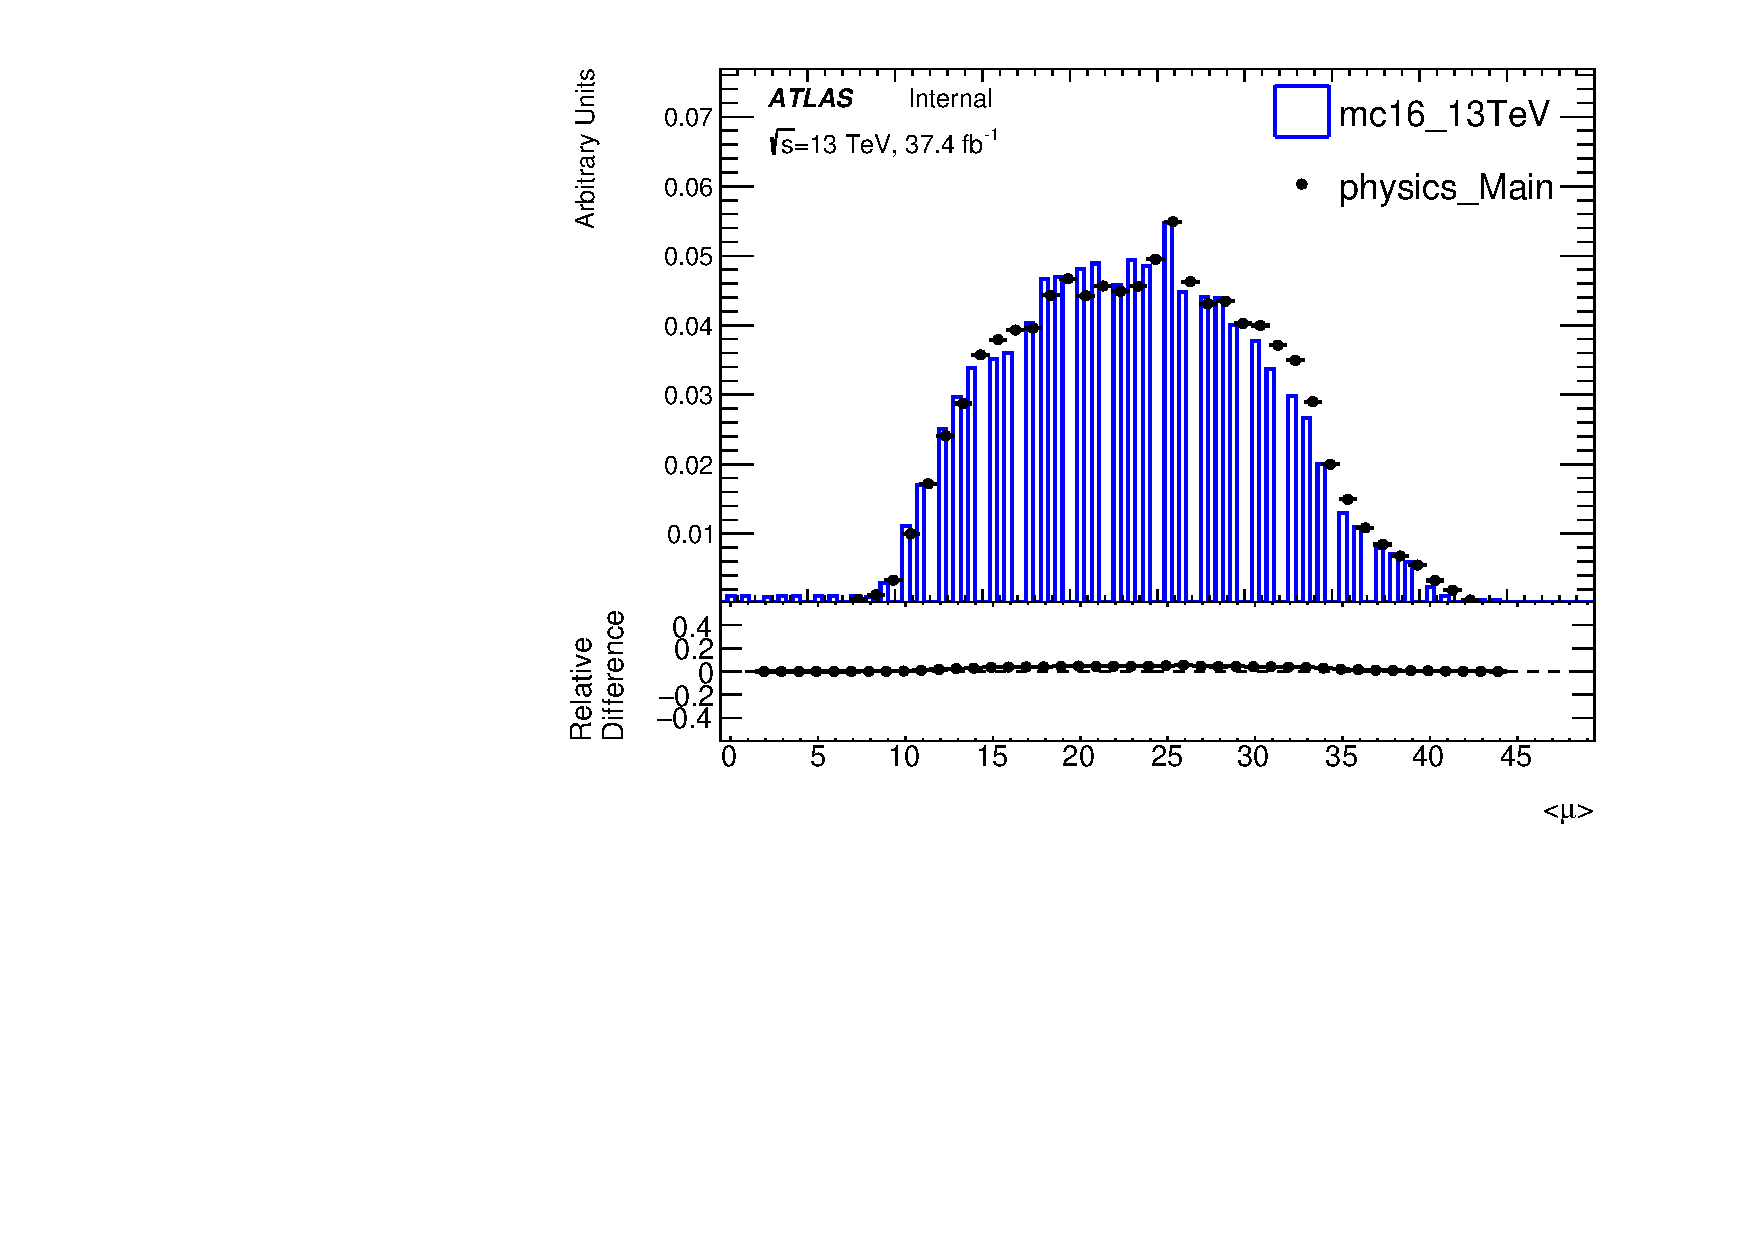
\includegraphics[width=0.45\textwidth]{figures/monitoring/resonant/2015-16/QG/newStudy_averageInteractionsPerCrossing_QGv01.pdf}}
% %
%
% \caption{Monitoring plots on %2016 data, 
% the QG resonant selection. (a) $H_T$, (b) $MH_T$ (missing transverse momentum calculated only from the jets in the event), (c) number of primary interaction vertices and (d) average interactions per bunch crossing.}
% \label{fig:QGmonitoring1}
%\end{figure}
%
% \begin{figure}[htb]
% \centering
%  \subfigure[] {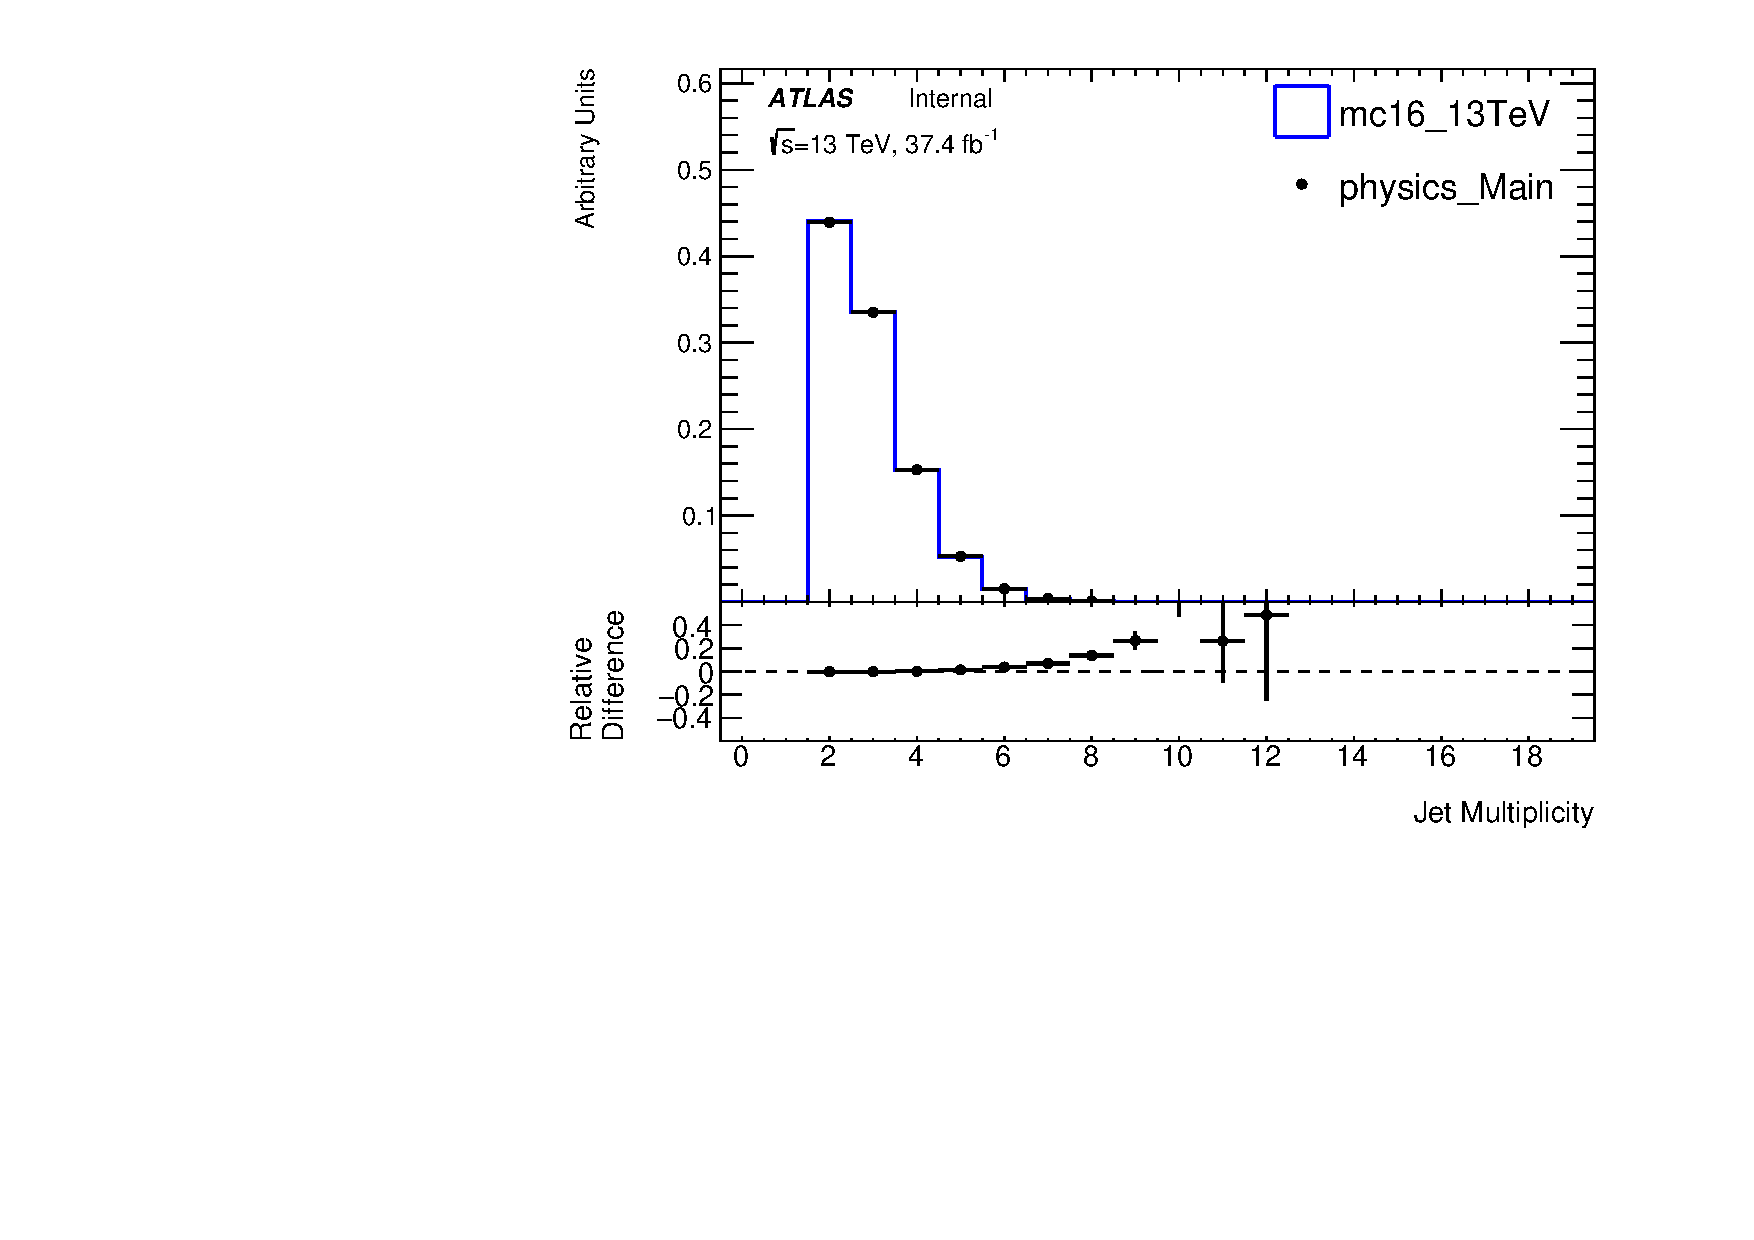
\includegraphics[width=0.45\textwidth]{figures/monitoring/resonant/2015-16/QG/newStudy_njets_QGv01.pdf}}
% \subfigure[] {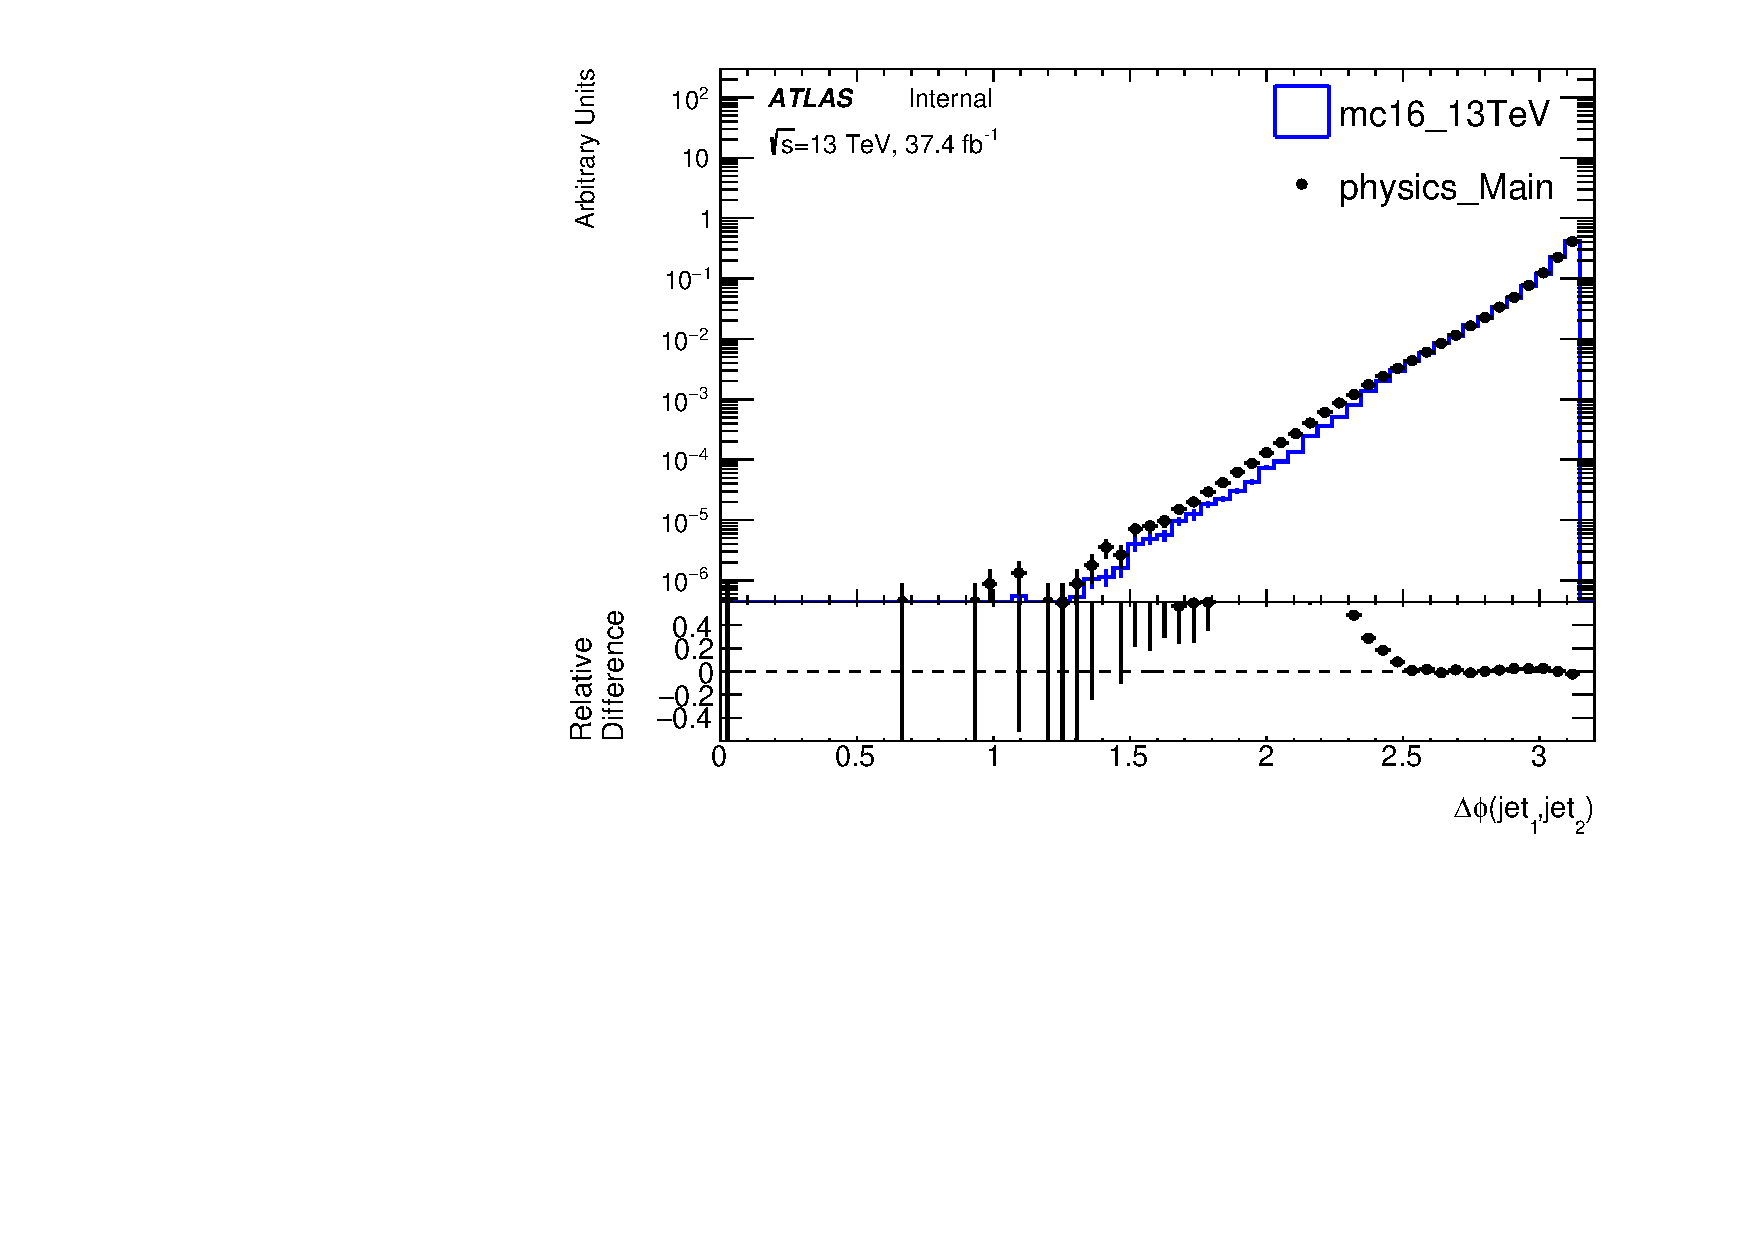
\includegraphics[width=0.45\textwidth]{figures/monitoring/resonant/2015-16/QG//newStudy_deltaPhi_logY_QGv01.pdf}}
% %
% \subfigure[] {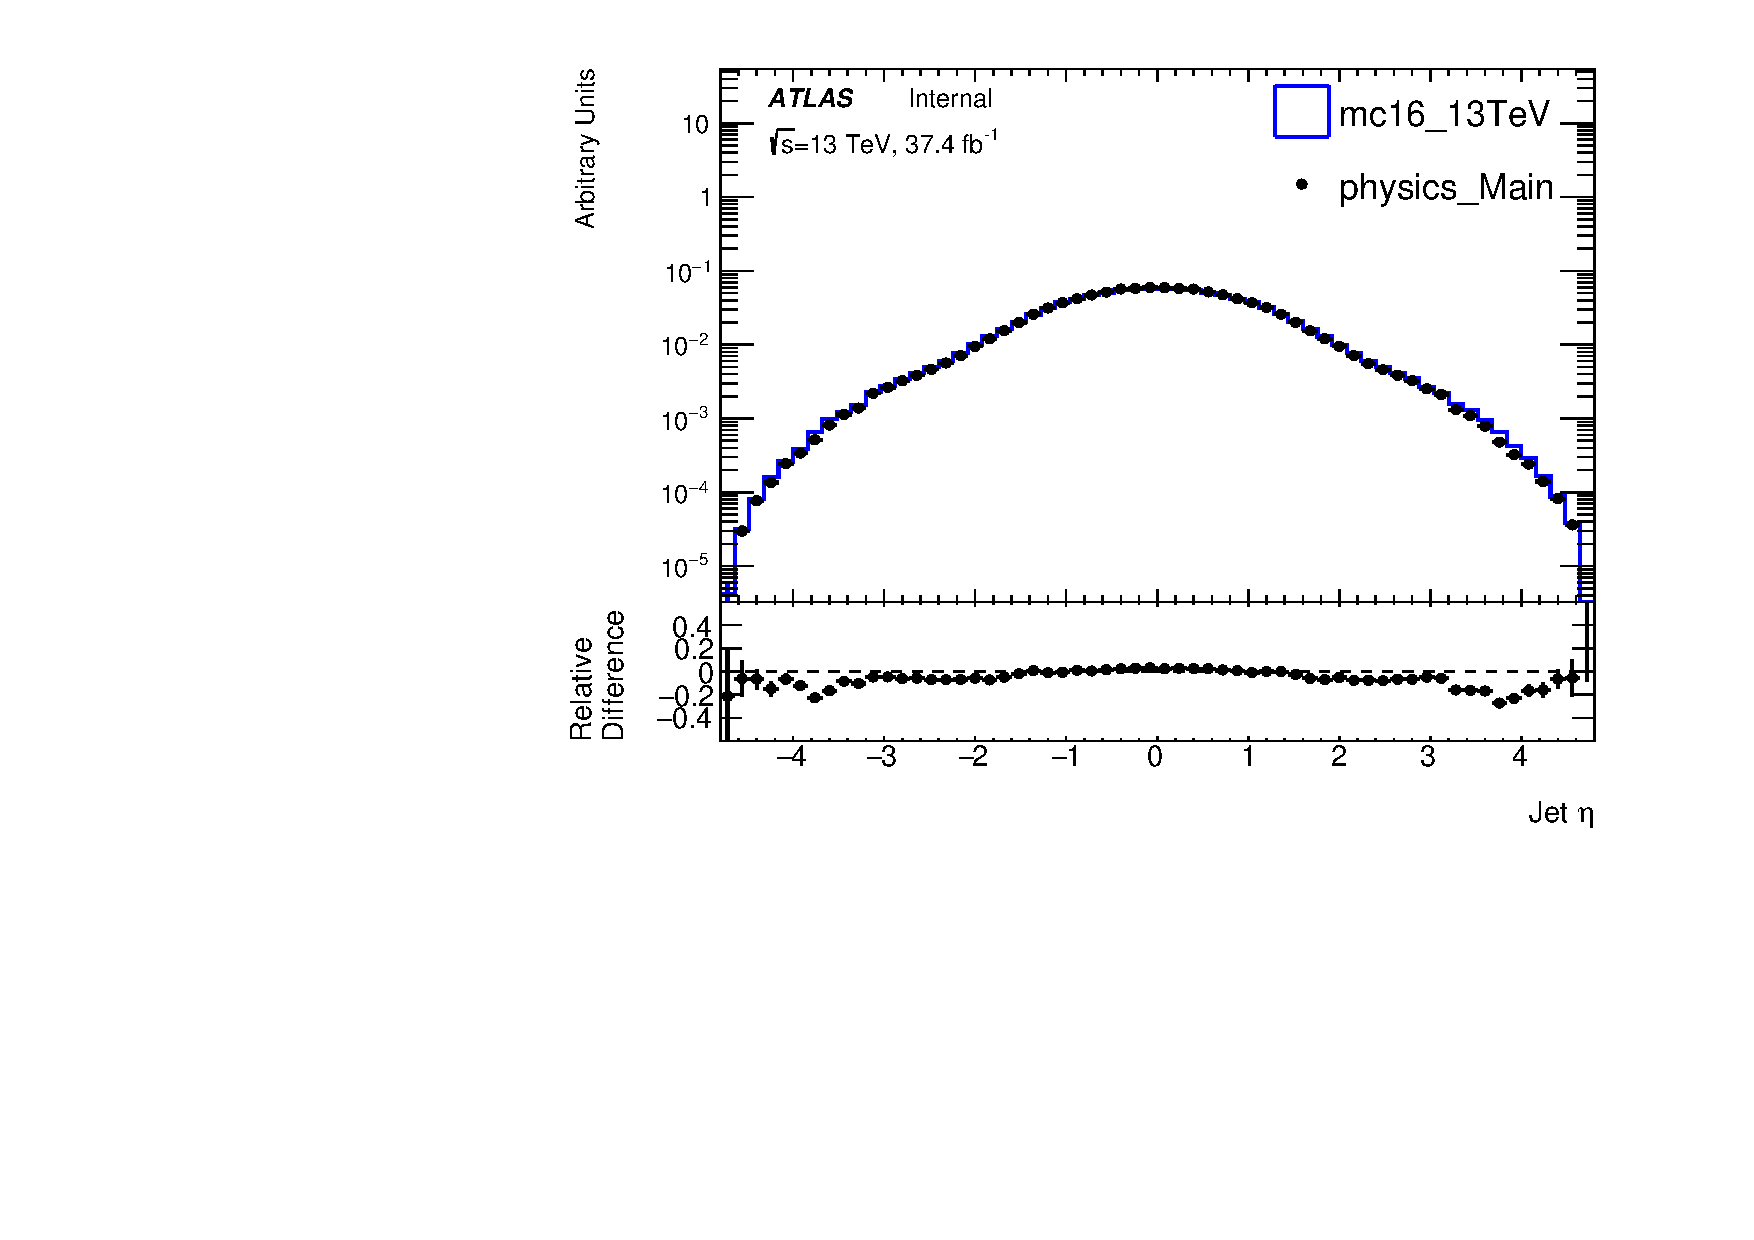
\includegraphics[width=0.45\textwidth]{figures/monitoring/resonant/2015-16/QG/newStudy_jet_eta_logY_QGv01.pdf}}
% \subfigure[] {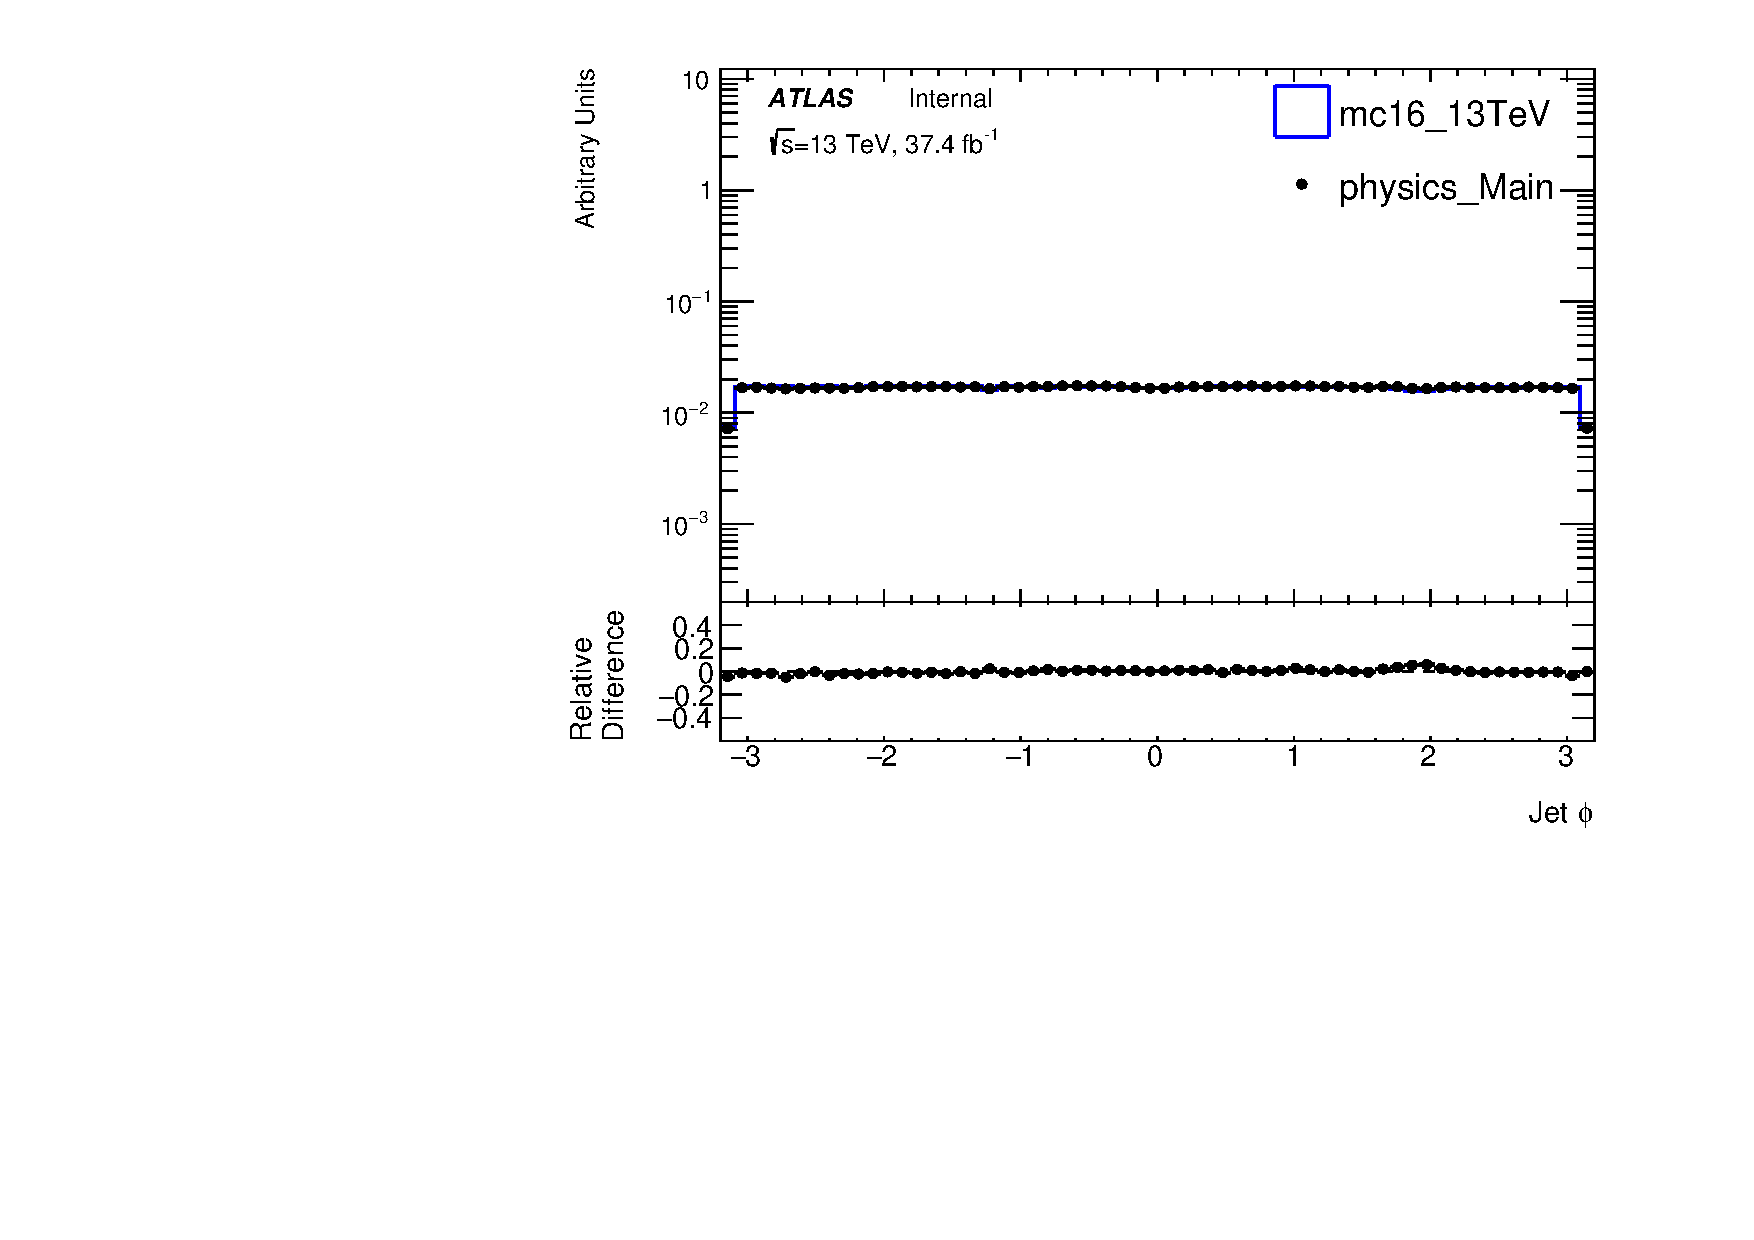
\includegraphics[width=0.45\textwidth]{figures/monitoring/resonant/2015-16/QG/newStudy_jet_phi_logY_QGv01.pdf}}
% %
% \subfigure[] {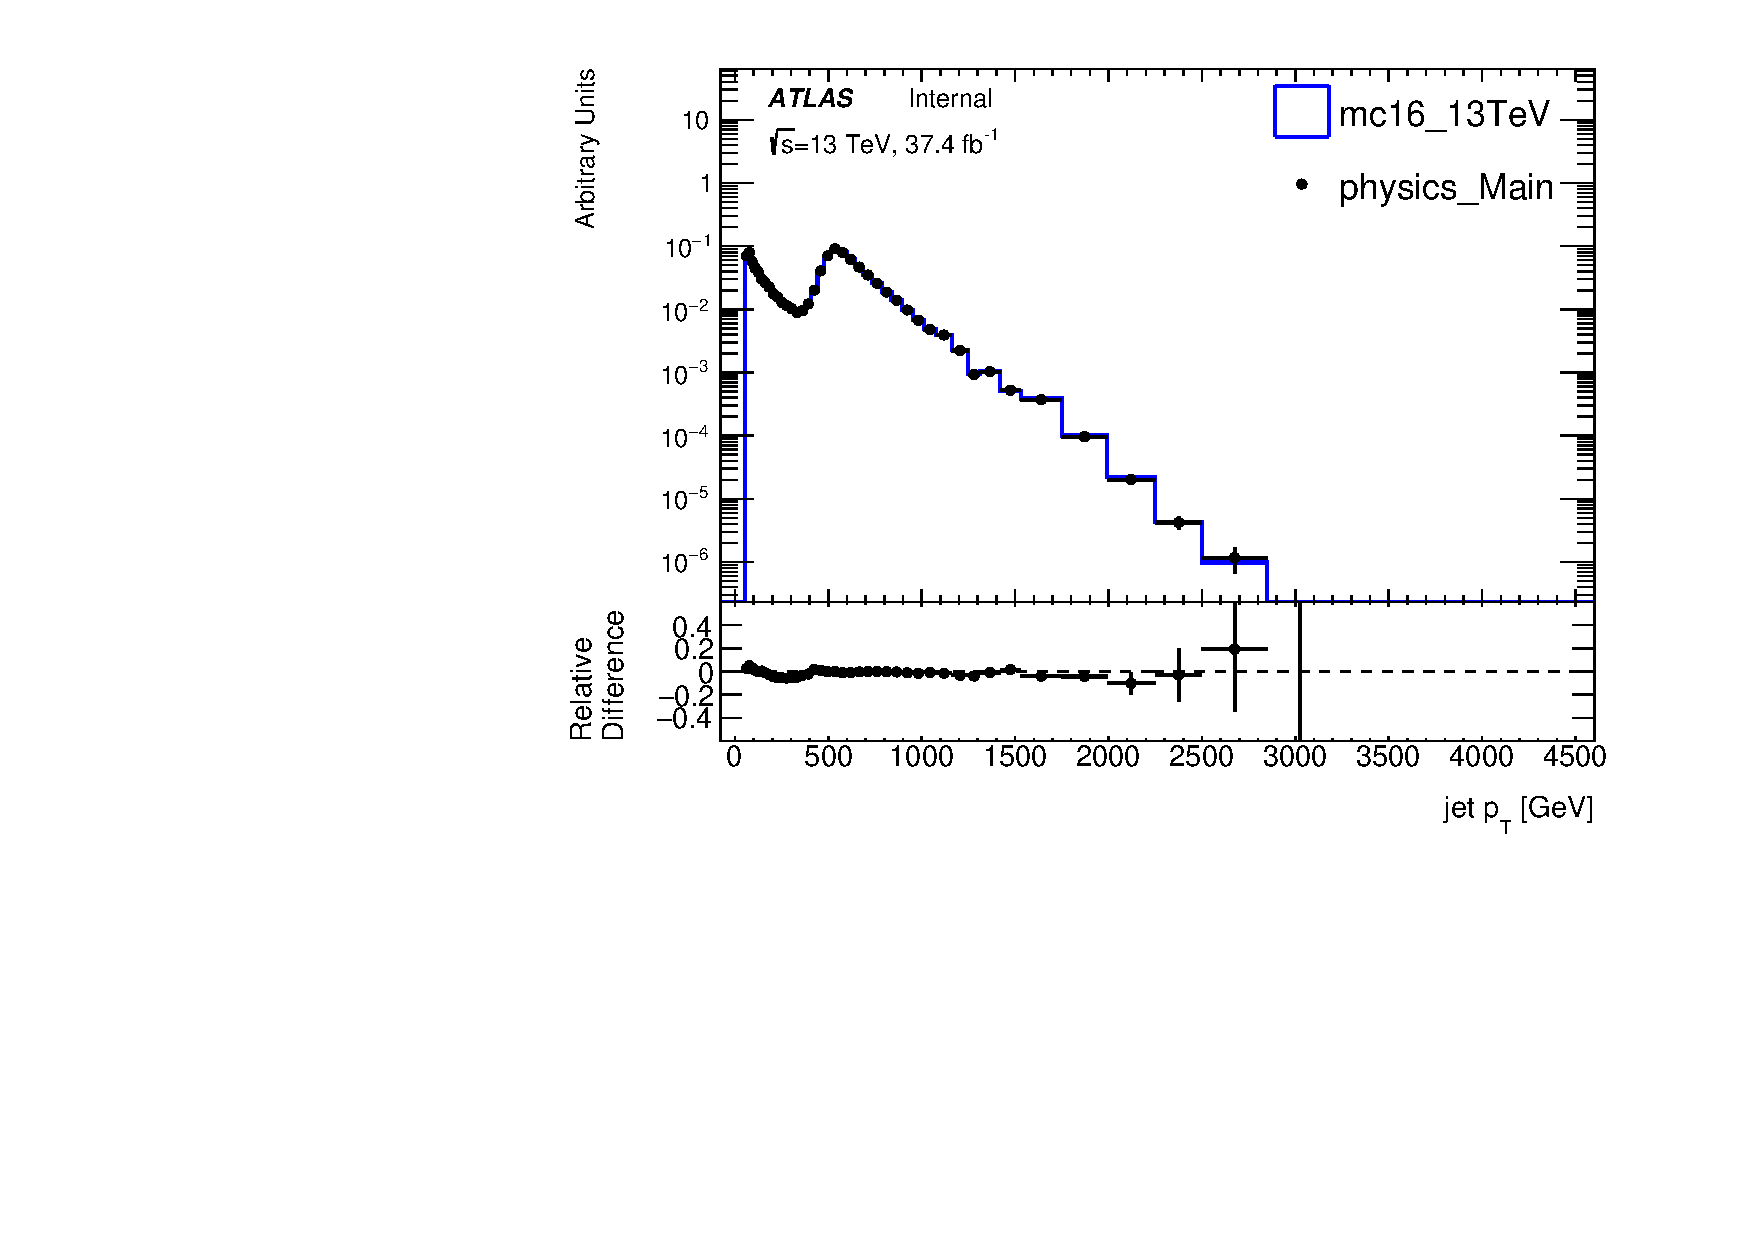
\includegraphics[width=0.45\textwidth]{figures/monitoring/resonant/2015-16/QG/newStudy_jet_pt_logY_QGv01.pdf}}
% \subfigure[] {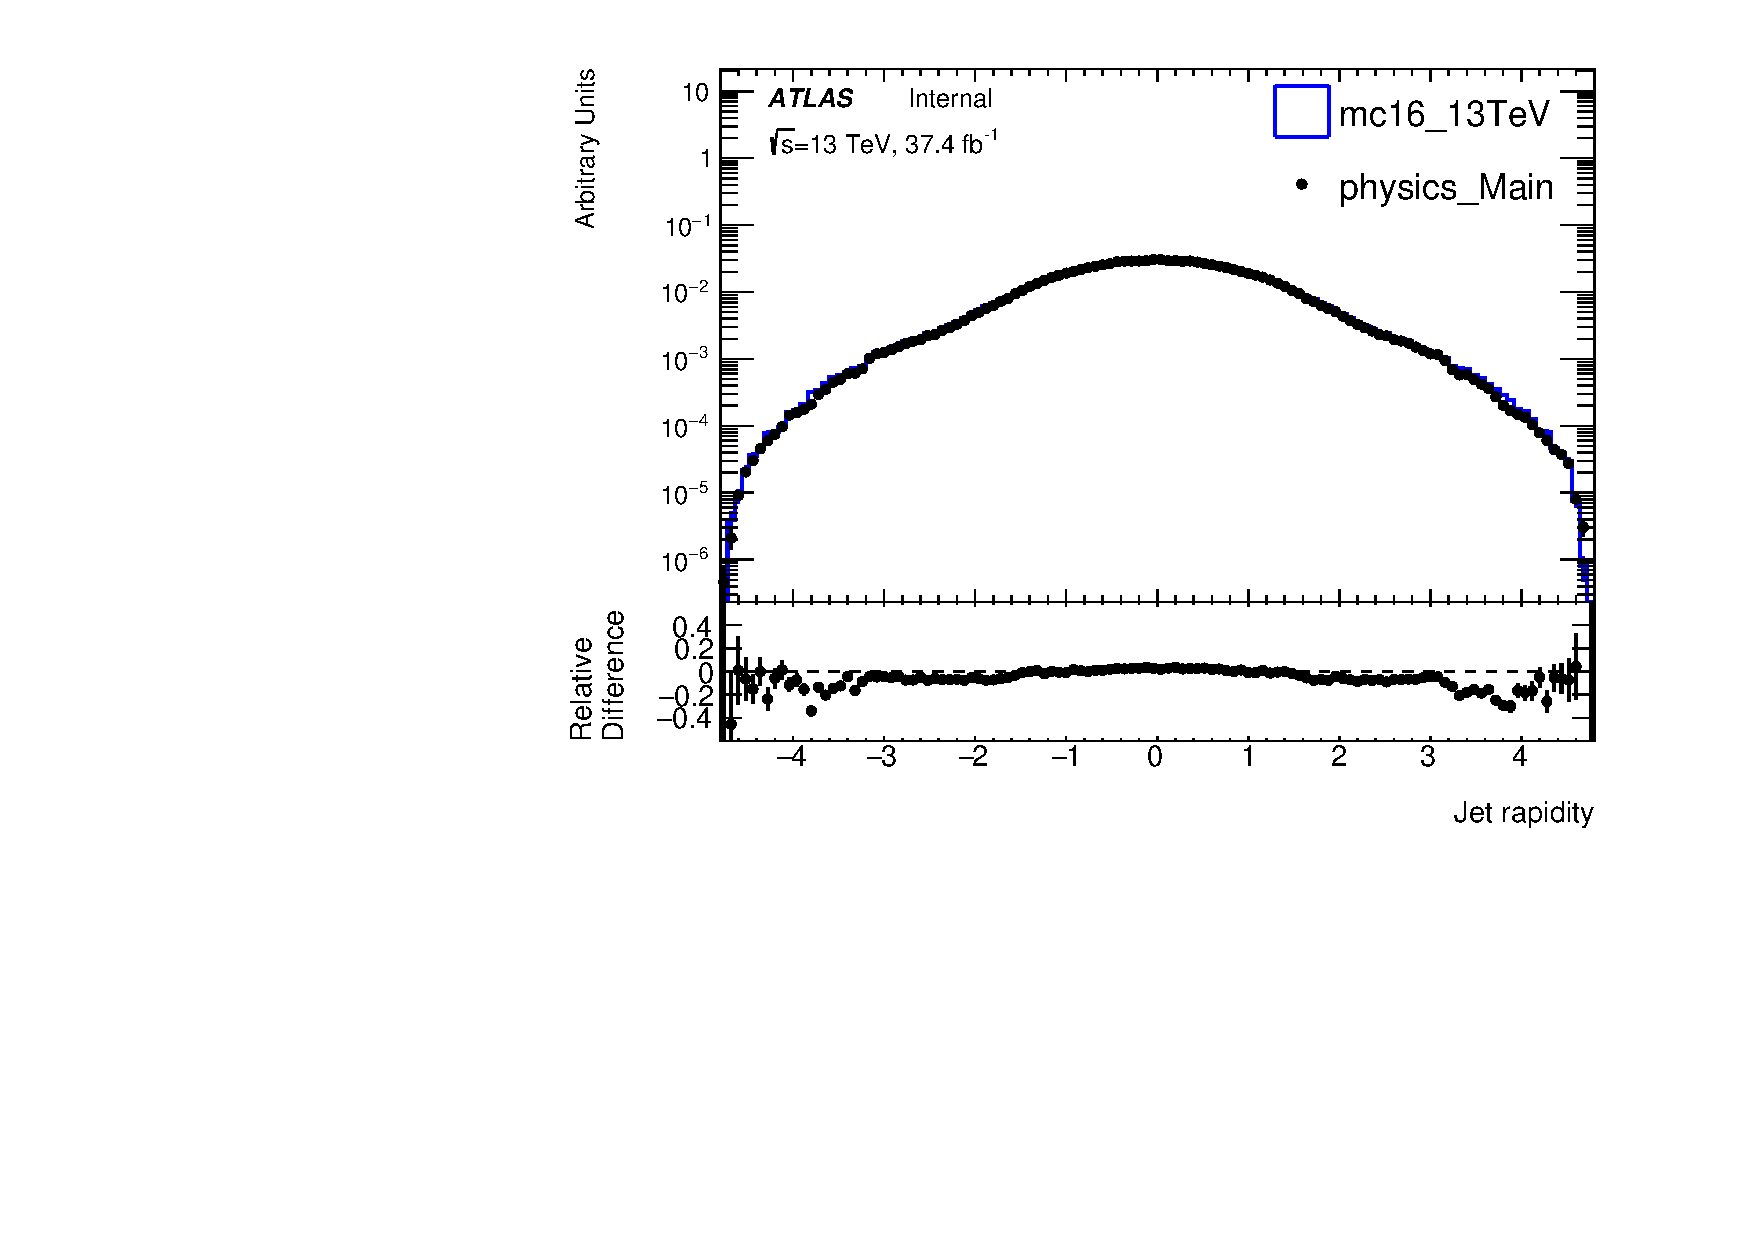
\includegraphics[width=0.45\textwidth]{figures/monitoring/resonant/2015-16/QG/newStudy_jet_rapidity_logY_QGv01.pdf}}
% %
%  \caption{Jet plots on %2016 data, 
%  the resonant selection. (a) number of jets (b) $\Delta\phi$ between the two jets (c) jet $\eta$
%  (d) jet $\phi$ (e) jet \pT\ (f) jet rapidity.  Fluctuations in the jet $phi$ distribution are attributable to dead modules in the tile calorimeter which lead to fewer jets in small slices of the detector.}
% \label{fig:QGmonitoring5}
%\end{figure}
%
%
% \begin{figure}[htb]
% \centering
% %
% \subfigure[] {\includegraphics[width=0.45\textwidth]{figures/monitoring/resonant/2015-16/QG/newStudy_mjj_logY_QGv01.pdf}}
% \subfigure[] {\includegraphics[width=0.45\textwidth]{figures/monitoring/resonant/2015-16/QG/newStudy_pTjj_logY_QGv01.pdf}}
% %
% \subfigure[] {\includegraphics[width=0.45\textwidth]{figures/monitoring/resonant/2015-16/QG/newStudy_yBoost_logY_QGv01.pdf}}
% \subfigure[] {\includegraphics[width=0.45\textwidth]{figures/monitoring/resonant/2015-16/QG/newStudy_yStar_logY_QGv01.pdf}}
% \caption{Jet plots on %2016 data, 
% the resonant selection. (a) dijet invariant mass (b) dijet \pT\ (c) \yB{} (d) \ystar{}. }
% \label{fig:QGmonitoring6}
%\end{figure}
%
%\clearpage
%
%
%In this section a selection of kinematic and monitoring plots produced with the resonant selection on the GG dataset is shown 
%(Figures~\ref{fig:GGmonitoring1},  
%\ref{fig:GGmonitoring5}, \ref{fig:GGmonitoring6}). These plots are relative to \integLumi of data collected in 2015 and 2016.
% GRL has been applied here.
%
%\begin{figure}[htb]
% \centering
% \subfigure[] {\includegraphics[width=0.45\textwidth]{figures/monitoring/resonant/2015-16/GG/newStudy_HT_logY_GGv01.pdf}}
% \subfigure[] {\includegraphics[width=0.45\textwidth]{figures/monitoring/resonant/2015-16/GG/newStudy_MHT_logY_GGv01.pdf}}
% %
% \subfigure[] {\includegraphics[width=0.45\textwidth]{figures/monitoring/resonant/2015-16/GG/newStudy_NPV_GGv01.pdf}}
% \subfigure[] {\includegraphics[width=0.45\textwidth]{figures/monitoring/resonant/2015-16/GG/newStudy_averageInteractionsPerCrossing_GGv01.pdf}}
% %
%
% \caption{Monitoring plots on %2016 data, 
% the GG resonant selection. (a) $H_T$, (b) $MH_T$ (missing transverse momentum calculated only from the jets in the event), (c) number of primary interaction vertices and (d) average interactions per bunch crossing.}
% \label{fig:GGmonitoring1}
%\end{figure}
%
% \begin{figure}[htb]
% \centering
%  \subfigure[] {\includegraphics[width=0.45\textwidth]{figures/monitoring/resonant/2015-16/GG/newStudy_njets_GGv01.pdf}}
% \subfigure[] {\includegraphics[width=0.45\textwidth]{figures/monitoring/resonant/2015-16/GG//newStudy_deltaPhi_logY_GGv01.pdf}}
% %
% \subfigure[] {\includegraphics[width=0.45\textwidth]{figures/monitoring/resonant/2015-16/GG/newStudy_jet_eta_logY_GGv01.pdf}}
% \subfigure[] {\includegraphics[width=0.45\textwidth]{figures/monitoring/resonant/2015-16/GG/newStudy_jet_phi_logY_GGv01.pdf}}
% %
% \subfigure[] {\includegraphics[width=0.45\textwidth]{figures/monitoring/resonant/2015-16/GG/newStudy_jet_pt_logY_GGv01.pdf}}
% \subfigure[] {\includegraphics[width=0.45\textwidth]{figures/monitoring/resonant/2015-16/GG/newStudy_jet_rapidity_logY_GGv01.pdf}}
% %
%  \caption{Jet plots on %2016 data, 
%  the resonant selection. (a) number of jets (b) $\Delta\phi$ between the two jets (c) jet $\eta$
%  (d) jet $\phi$ (e) jet \pT\ (f) jet rapidity.  Fluctuations in the jet $phi$ distribution are attributable to dead modules in the tile calorimeter which lead to fewer jets in small slices of the detector.}
% \label{fig:GGmonitoring5}
%\end{figure}
%
%
% \begin{figure}[htb]
% \centering
% %
% \subfigure[] {\includegraphics[width=0.45\textwidth]{figures/monitoring/resonant/2015-16/GG/newStudy_mjj_logY_GGv01.pdf}}
% \subfigure[] {\includegraphics[width=0.45\textwidth]{figures/monitoring/resonant/2015-16/GG/newStudy_pTjj_logY_GGv01.pdf}}
% %
% \subfigure[] {\includegraphics[width=0.45\textwidth]{figures/monitoring/resonant/2015-16/GG/newStudy_yBoost_logY_GGv01.pdf}}
% \subfigure[] {\includegraphics[width=0.45\textwidth]{figures/monitoring/resonant/2015-16/GG/newStudy_yStar_logY_GGv01.pdf}}
% \caption{Jet plots on %2016 data, 
% the resonant selection. (a) dijet invariant mass (b) dijet \pT\ (c) \yB{} (d) \ystar{}. }
% \label{fig:GGmonitoring6}
%\end{figure}
%
%\clearpage


\subsection{Analysis cutflow}
%\label{sec:data_cutflow}

This section and the next present the analysis cutflows. Cutflows obtained on
Run-2 data are presented in Tables~\ref{tab:cutFlow_resonance_run2} and 
\ref{tab:cutFlow_wstar_run2}.

\begin{table}[htbp]
	\centering
	\begin{tabular}{l|c|c}
		\hline\hline
		Selection criteria & $N_{events}$ & rel. decrease (\%) \\
		\hline
		all      &	4738142726	&	0.00	\\
		Apply GRL 	& 	4442605390        & 	-6.24	 \\
		Cleaning	 & 	4379077017	 & 	-1.43	 \\
		HLT j420	 & 	266104885	 & 	-93.9	 \\
		jet pre-selection	 &     259157844         &      -2.61    \\
		$|\Delta\phi| > 1.0$	 & 		 & 		 \\
		$|\ystar| < 0.6$	 & 		 & 		 \\
		$\mjj>1100~\GeV$	 & 		 & 		 \\
		\hline\hline
	\end{tabular}
	\caption{Cutflow for
		events with H$^\prime$ cuts:  $m_{jj}>1100~\GeV$, and $|\ystar|<0.6$. .
		\label{tab:cutFlow_resonance_run2} }
\end{table}

\begin{table}[htbp]
	\centering
	\begin{tabular}{l|c|c}
		\hline\hline
		Selection criteria & $N_{events}$ & rel. decrease (\%) \\
		\hline
		all      &	4738142726	&	0.00	\\
		Apply GRL 	& 	4442605390        & 	-6.24	 \\
		Cleaning	 & 	4379077017	 & 	-1.43	 \\
		HLT j420	 & 	266104885	 & 	-93.9	 \\
		jet pre-selection	 &     259157844        &      -2.61    \\
		$|\Delta\phi| > 1.0$	 & 		 & 		 \\
		$|\ystar| < 0.8$	 & 		 & 	 \\
		$\mjj>1133~\GeV$	 & 		 & 	 \\
		\hline\hline
	\end{tabular}
	\caption{Cutflow for
		events with string resonance cuts:  $\mjj>1133~\GeV$, and $|\ystar|<0.8$. .
		\label{tab:cutFlow_wstar_run2} }
\end{table}

Joyti confirms these tables up to the row ``jet pre-selection'', but after that he has three additonal rows.
We don't know what TriggerEfficieincy is yet there are events lost. The $|\ystar|$ cut can be removed at we don't make it and no events are lost. 
But the last row is worrysome that no events are lost.
And the origial tables make no mention or requiring at least two jets.

\begin{table}[htbp]
	\centering
	\begin{tabular}{l|c|c}
		\hline\hline
		Selection criteria & $N_{events}$ & rel. decrease (\%) \\
		\hline
		TriggerEfficiency: N/A & 259157844 &\\
		$|\ystar|$: N/A        & 259157844 &\\
		Leading jet $\pT \ge 380\GeV$ & &\\
		Sub-leading jet $\pT \ge 150\GeV$ & 259157844 &\\
		Jet multiplicity $\ge 2$ & &\\
		\hline\hline
	\end{tabular}
\end{table}

%\begin{table}[htbp]
%\sisetup{group-minimum-digits=4}
%\centering
%\begin{tabular}{lSS}
%Data Set 	& \multicolumn{1}{c}{$N_{\mathrm{events}}$} 	& \multicolumn{1}{c}{Fraction (\%)} \\
%\hline
%QQ 			& 313113 		& 4.2\\
%QG			& 2275205 		& 30.2\\
%GG			& 4945115	  	& 65.6\\
%\hline\hline
%\end{tabular}
%\caption{Fraction of 2015+12016  events with resonance cuts in the quark-quark (QQ), quark-gluon (QG) and gluon-gluon (GG)
%sub-samples. 
%\label{tab:cutFlow_sample_fractions} }
%\end{table}




